\makeatletter
\let\my@xfloat\@xfloat
\makeatother

%\documentclass{macthesis}
\documentclass[twoside]{Styles/macthesis}
\listfiles
%\usepackage{xspace}
\usepackage{amsmath}
\usepackage{amssymb}
%\usepackage{multirow}
\usepackage{Styles/natbib}
\usepackage{chapterbib}
\usepackage{graphicx}
\usepackage{Styles/deluxetable}
%\usepackage{subfigure}
%\usepackage{lscape}
%\usepackage{supertabular}
%\usepackage{appendix}
\usepackage{longtable}
%\usepackage{cite}
\usepackage{listings}
%\usepackage{subfigure}
\usepackage{glossary}
\usepackage{pdfpages}
\usepackage{mhchem}
\usepackage{upgreek}
\usepackage{subcaption}
\usepackage{gensymb}
%\renewcommand{\topfraction}{0.85}
%\renewcommand{\textfraction}{0.1}


%

%
\def\hlf  {{\textstyle {1\over2} }}
\def\fD   {\mathfrak D}
\def\vD   {v_{\mathfrak D}}
\def \bY  {\color{blue} Yes}
%\def\mnras {{MNRAS}}
%\def\aap {{A\&A}}
%\def\apj {{ApJ}}
%\def\apjl {{ApJL}}
\def \rN  {\color{red} No}
\def\oii{[O{\sc ii}]}
\def\ewoii{$W_{\rm \circ}$(\oii)}

% \newif\ifpdf
% \ifx\pdfoutput\undefined
%         \pdffalse
% \else
%         \pdfoutput=1
%         \pdftrue
% \fi
% \ifpdf
%         \usepackage[pdftex]{graphicx}
% %        \usepackage[pdftex]{rotating}
% \else
%         \usepackage{rotating}
%         \usepackage{epsf}
% 	\usepackage{graphicx}
% \fi
% \ifpdf
%         \pdfpageheight=11in
%         \pdfpagewidth=8.5in
%         \pdfinfo{ 
%                 /Title (Thesis)
%                 /Subject (Thesis)
%                 /Author (Iman Author)
%                 }
% \fi
% \usepackage{epsf,graphicx,rotating}
\usepackage{Styles/mypig}
%\usepackage{mycite}
\usepackage{verbatim}
%\renewcommand{\thefootnote}{\fnsymbol{footnote}}
% draft written across paper (only is ps mode)
%\usepackage{draftcopy}
%\draftcopyName{Work in Progress}{105}
%

%johnny newtron's xfloat hack via latex-community.org

\makeatletter
\def\@xfloat#1[#2]{
    \my@xfloat#1[#2]%
    \def\baselinestretch{1}%
    \@normalsize \normalsize
}
\makeatother  


\begin{document}

% define the various title-page, preamble variables

\newcommand{\firstname}{Jonathan}
\newcommand{\middlename}{H.}
\newcommand{\lastname}{Newton}
\newcommand{\degrees}{B.A.}
\newcommand{\thetitle}{Dust and Gas in NGC3627 Using Observations from SCUBA-2}
\newcommand{\halftitle}{Dust and Gas in NGC3627}
\newcommand{\thedegree}{Master of Science}
\newcommand{\shortdegree}{M.Sc.}
\newcommand{\currentmonth}{August}
\newcommand{\currentyear}{2014}
\newcommand{\department}{Physics and Astronomy}
\newcommand{\shortdepartment}{Physics and Astronomy}
\newcommand{\theuniversity}{McMaster University}
\newcommand{\bindingyear}{2014}
\newcommand{\submissionyear}{2014}
\newcommand{\submissionmonth}{August}
\newcommand{\supervisor}{Christine D. Wilson}
\newcommand{\thelocation}{Hamilton, Ontario}
\newcommand{\degreefrom}{Western Kentucky University}


\newcommand{\firstpages}{\pageref{frontmatterpages}}
\newcommand{\lastpages}{\pageref{finalpage}}


\halftitlepage
\thesistitle
\descriptivenotes

\begin{abstract} 

Saw some dust and wanted to do something about it!

Ultra/Luminous infrared galaxies (U/LIRGs) are some of the most amazing systems in the local universe exhibiting extreme star formation triggered by mergers. Since molecular gas is the fuel for star formation, studying the warm, dense gas associated with star formation is important in understanding the processes and timescales controlling star formation in mergers. We have used high resolution ($\sim$2.3") observations of the local LIRG Arp 299 (D= 44Mpc) to map out the physical properties of the molecular gas. The molecular lines $^{12}$CO J=3-2, $^{12}$CO J=2-1 and $^{13}$CO J=2-1 were observed with the Submillimeter Array and the short spacings of the $^{12}$CO J=3-2 and J=2-1 observations have been recovered using James Clerk Maxwell Telescope single dish observations. We use the radiative transfer code RADEX to measure the physical properties such as density and temperature of the different regions in this system. The RADEX solutions of the two galaxy nuclei, IC 694 and NGC 3690, show two gas components: a warm  moderately dense gas with $T_{kin}$ $\sim$ 30-500 K (up to 1000 K for NGC 3690) and $n$(H$_{2}$) $\sim$ 0.3 - 3 $\times$ 10$^{3}$ cm$^{-3}$ and a cold dense gas with $T_{kin}$ $\sim$ 10-30 K and $n$(H$_{2}$) $>$ 3 $\times$ 10$^{3}$ cm$^{-3}$. The overlap region is shown to have a well-constrained solution with $T_{kin}$ $\sim$ 10-30 K and $n$(H$_{2}$) $\sim$ 3-30 $\times$ 10$^{3}$ cm$^{-3}$. We estimate the gas masses and star formation rates of each region in order to derive molecular gas depletion times. The depletion time of each region is found to be about 2 orders of magnitude lower than that of normal spiral galaxies. This can be probably explained by a higher fraction of dense gas in Arp 299 than in normal disk galaxies. 


\end{abstract}




\dedication{To my family and Poly.}
\begin{acknowledgement}

\textit{When life looks like easy street, there is danger at your door... -Robert Hunter}

Thank Chris and group members of course.  Don't forget Christian!

\end{acknowledgement}

\tableofcontents
\listoffigures
%\listofequations%very optional
\listoftables
%\label{lastfirst} 

%Ultra/Luminous infrared galaxies (U/LIRGs) are some of the most amazing systems in the local universe exhibiting extreme star formation triggered by mergers. Since molecular gas is the fuel for star formation, studying the warm, dense gas associated with star formation is important in understanding the processes and timescales controlling star formation in mergers. We have used high resolution ($\sim$2.3") observations of the local LIRG Arp 299 (D= 44Mpc) to map out the physical properties of the molecular gas. The molecular lines $^{12}$CO J=3-2, $^{12}$CO J=2-1 and $^{13}$CO J=2-1 were observed with the Submillimeter Array and the short spacings of the $^{12}$CO J=3-2 and J=2-1 observations have been recovered using James Clerk Maxwell Telescope single dish observations. We use the radiative transfer code RADEX to measure the physical properties such as density and temperature of the different regions in this system. The RADEX solutions of the two galaxy nuclei, IC 694 and NGC 3690, show two gas components: a warm  moderately dense gas with $T_{kin}$ $\sim$ 30-500 K (up to 1000 K for NGC 3690) and $n$(H$_{2}$) $\sim$ 0.3 - 3 $\times$ 10$^{3}$ cm$^{-3}$ and a cold dense gas with $T_{kin}$ $\sim$ 10-30 K and $n$(H$_{2}$) $>$ 3 $\times$ 10$^{3}$ cm$^{-3}$. The overlap region is shown to have a well-constrained solution with $T_{kin}$ $\sim$ 10-30 K and $n$(H$_{2}$) $\sim$ 3-30 $\times$ 10$^{3}$ cm$^{-3}$. We estimate the gas masses and star formation rates of each region in order to derive molecular gas depletion times. The depletion time of each region is found to be about 2 orders of magnitude lower than that of normal spiral galaxies. This can be probably explained by a higher fraction of dense gas in Arp 299 than in normal disk galaxies. 

\pagestyle{myheadings}
\pagenumbering{arabic}

\chapter{Introduction}\label{intro}

\section{The Physical Processes of Star Formation} %need to change this since it deals with formation of H2

Star formation is one of the fundamental processes in astrophysics that affects not just stellar and planetary formation but also dictates the behavior in galaxy formation and evolution \citep{kennicutt2012}.  The study of star formation itself can be broken into several areas such as: the processes that trigger collapse and how the collapse behaves, dictating how and what type of stars can form from a given region or cloud, or how the inflow of new material can alter current star forming environments.  These different sub-branches of star formation are conveniently sorted into hierarchal schemes that range from Mpc scales seen in gas accretion from the intergalactic medium, to properties of accretion disks on scales of the order $R_\odot$ or AU\citep{kennicutt2012}.  In this body of work we focus on the physical properties of the dust and abundance of gas in the giant molecular cloud (GMC) phase of star formation prior to stellar collapse or fragmentation.  However based on the resolution of our target galaxy, we will not be able to examine individual GMCs instead we will need to focus our work on giant molecular associations (GMAs).

\subsection{GMC Formation}

After the intergalactic gas has accreted into a host galaxy, it will eventually condense and begin to form a GMC \citep{kennicutt2012}.  The condensation of this gas leads to the formation of molecular clouds.  The dominant process of GMC formation is divided between two camps; either a ``bottom-up'' or ``top-down'' formation scenario \citep{mckee2007}.  The bottom-up scenario consists of small clouds of cold HI coagulating to eventually form a GMC \citep{field1965, kwan1979}.  The major concern with the bottom-up scenario is if we include heating mechanisms in the cloud, coagulation will cease before the observed masses are reached \citep{mckee2007}.  In fact, the time scales required to form a cloud typical of what we observe would take around $10^8$ years to accumulate a minimum of 10$^5$ M$_\odot$, which is much greater than the expected GMC lifetime \citep{mckee2007}.  %try to find typical gmc lifetime 

The alternative formation scenario, top-down, postulates the GMC formation comes from instabilities in the diffuse ISM causing the clouds to collapse from their surrounding medium \citep{mckee2007}.  Two main instabilities are thought to be responsible for the collapse.  The first type of instability is a Parker instability, which involves distortion of magnetic fields lines in the mid plane of the galaxy, and at these distortions gas will begin to accumulate \citep{parker1966, dobbs2013}.  The second instability responsible for collapse comes in the style of a more complex Jeans instability which is determined further by the amount of rotational shear present \citep{mckee2007}.  If a strong rotational shear is present, such as in the inter arm region of a spiral galaxy, then a process known as swing amplification will occur \citep{mckee2007}.  If no rotational shear is present, such as the inner regions of a galaxy or spiral arms, then the collapse can be attributed to a magneto-Jeans instability \citep{elmegreen1987,kim2001}.

\subsection{Molecular Hydrogen Formation}\label{h2form}

Regardless of either collapse or coagulation, molecular hydrogen is being formed inside the cloud.  The formation of molecular hydrogen can be summarized using either the two body reaction, three body reaction, formation using a free electron or proton, or surface formation \citep{krumholz2014}.  The two body formation scenario is the simplest reaction using two hydrogen atoms to produce molecular hydrogen, reaction \ref{eq:2bod}.

\begin{equation}\label{eq:2bod}
  \ce{H + H -> H_2}
\end{equation}

However the two body formation is not the major mechanism in the formation of H$_2$ due to the requirement of a forbidden photon that arises from the combination of hydrogen atoms in the ground state \citep{gould1963}.  If one of the hydrogen atoms is excited, the transition can occur and molecular hydrogen is formed, but the amount of excited hydrogen atoms in the temperature ranges typical of the cold and warm phases of the ISM are expected to be nearly nonexistent \citep{krumholz2014}.

The second formation scenario listed, the three body formation, involves three hydrogen atoms coming together to form molecular hydrogen with a spare hydrogen atom shown in reaction \ref{eq:3bod}.

\begin{equation}\label{eq:3bod}
  \ce{3H -> H_2 + H}
\end{equation}

The required density for the three body formation to occur is on the order of 10$^8$ cm$^{-3}$ \citep{palla1983,abel1997}, while the typical GMC density is on the order of 300 cm$^{-3}$.  The disparity between these densities eliminates any possibility of this being the primary mechanism to form molecular hydrogen. 

An alternative to the two or three body reactions uses either an electron or proton to ionize the hydrogen forming either H$^-$ or H$_2^+$ \citep{krumholz2014}.  The chemical reaction involving an electron is shown in reaction \ref{eq:eform} and reaction utilizing a proton is shown in reaction \ref{eq:pform}
\begin{equation}\label{eq:eform}
  \begin{split}
    \ce{H + \it{e} -> H^- + \it{h\nu}} \\
    \ce{H^- + \it{e} -> H_2 + \it{e}}
  \end{split}
\end{equation}

\begin{equation}\label{eq:pform}
  \begin{split}
    \ce{H + H^+ -> H^+_2 + \it{h\nu}} \\
    \ce{H^+_2 + H -> H_2 + H^+}
  \end{split}
\end{equation}

The main limitation of the free electron/proton formation mechanism is an undersupply of free electrons and protons.  Typical Milky Way conditions show that regions $>$1 cm$^{-3}$ have free electron and proton densities $<$10$^{-4}$ cm$^{-3}$ \citep{wolfire2003}.  Secondly, the H$^-$ ion in reaction \ref{eq:eform} is more likely to interact with a stray photon than an electron resulting in the ion returning to the atomic state \citep{glover2003}.  While we observe singly ionized hydrogen regions, HII regions, only a small fraction of the region will successfully produce molecular hydrogen.

While the free electron/proton formation method is suspected to be the primary H$_2$ catalyst in the early universe \citep{herbst2005}, at low redshifts the formation of molecular hydrogen on the surface of dust grains is the dominant mechanism of formation \citep{krumholz2014}.  The surface formation of molecular hydrogen will occur when a hydrogen atom strikes a dust grain and successfully sticks to the grain.  The hydrogen then will then interact with another hydrogen atom to form H$_2$ and be ejected from the dust particle after the reaction has occurred \citep{pirronello1997}.  The same process occurs on the dust grain as the two body formation, but  the dust grain will act as a medium to absorb the energy that would create the forbidden photon \citep{krumholz2014}.

%it would be a good idea to explain the requirements of the dust since not all dust can form H_2

With a dominant mechanism for molecular hydrogen formation, a reaction rate can be defined based on the cross section of the grain, $\Sigma_{gr}$, a striking probability dependent on the temperature of the observed dust, S(T), the probability of molecular hydrogen forming on the grain, $\upepsilon_{H_2}$, the density of free hydrogen in the GMC, n$_H$, and the density of hydrogen attached to the grain surface, n$_H{_0}$ \citep{krumholz2014}.  Scaling this with the integrated collisional probability of a Maxwellian gas, a reaction rate is determined to be equation \ref{eq:reac_rate} where k$_b$ is the Boltzmann constant, T is the temperature, and m$_H$ is the mass of the hydrogen atom.

\begin{equation}\label{eq:reac_rate}
  \frac{dn_{H_2}}{dt} = \frac{1}{2}\left(\frac{8k_bT}{\pi m_H}\right)^\frac{1}{2}\Sigma_{gr}S\left(T\right)\upepsilon_{H_2}n_{H}n_{H_0}
\end{equation}

Equation \ref{eq:reac_rate} is often simplified to equation \ref{eq:reac_rate_sm} by introducing a variable known as the formation rate, $\mathcal{R}_{gr}$, that is constrained using the column densities CI, CII, HI, H$_2$.  Typical reaction rates for the Milky Way have been found to be 3x10$^{-17}$cm$^3$s$^{-1}$ \citep{jura1975, gry2002, wolfire2008}.

\begin{equation}\label{eq:reac_rate_sm}
  \frac{dn_{H_2}}{dt} = \mathcal{R}_{gr}n_H n_{H_0}
\end{equation}

\subsection{Dissociation of Molecular Hydrogen}\label{h2destroy}

When the molecular hydrogen has formed, it is still susceptible to photodissociation from far ultra-violet (FUV) photons.  The energy required for a single photon to break the bonds of molecular hydrogen is 14.5 eV \citep{krumholz2014}.  Conveniently, this is also enough energy to excite atomic hydrogen, so photodissasociation using a single photon is highly unlikely due to the abundance of HI in the ISM \citep{krumholz2014}.  However, a photon with an energy of 11-13.6 eV will not be able to excite atomic hydrogen, but will be able to excite the molecular hydrogen to its first and second excitation levels, the Lyman and Werner bands respectively.  The excited H$_2$ will eventually settle via photon emission to its ground state with a finite probability of returning to two hydrogen atoms rather than maintaing its molecular state \citep{krumholz2014}.

%need a little more in this use the draine 2011 book
A dissociation rate, $\zeta_{diss}$, can be obtained by scaling the total excitation rate, $\zeta_{exc}$, by the fraction of excited hydrogen molecules that will settle to an atomic ground state \citep{krumholz2014}.  The total excitation rate is found by summing each of individual excitations from the ground state e.g. $\zeta_{exc,0-1}$, $\zeta_{exc,0-2}$.  In the Milky Way's diffuse ISM, the interstellar radiation field is 6-9x10$^{-14}$ erg cm$^{-3}$ over the range of 6-13.6 eV resulting in $\zeta_{exc} \approx 3\times10^{-10}$s$^{-1}$ \citep{draine2011}.  The expected fraction of H$_2$ to disassociate is between 0.11 and 0.13 resulting in $\zeta_{diss}\approx4\times10^{-11}$s$^{-1}$\citep{draine2011}.
Equating the formation and dissociation rates and then solving for a molecular hydrogen vs atomic hydrogen ratio gives in equation \ref{eq:fd_eq1} \citep{krumholz2014}.  From equation \ref{eq:fd_eq1} we can see, in the diffuse medium, atomic hydrogen is far more abundant than molecular hydrogen, as expected.

\begin{equation}\label{eq:fd_eq1}
  \begin{split}
    \zeta_{diss} n_{H_2} & = \mathcal{R}n_{H_0}n_H \\
    \frac{n_{H_2}}{n_H} & = \frac{\mathcal{R}n_{H_0}}{\zeta_{diss}} \\
                        & = 8\times10^{-6}\left(\frac{4\times10^{-11}s^{-1}}{\zeta_{diss}}\right)\left(\frac{n_{H_0}}{10cm^{-3}}\right)
  \end{split}
\end{equation}

However, as the density of the gas increases via collapse or coagulation, the optical depth will also increase limiting the amount of FUV photons able to penetrate into the core of the cloud, a process known as shielding \citep{draine2011}.  This shielding will aid in the decrease of $\zeta_{diss}$ which will increase the value in equation \ref{eq:fd_eq1}.  The increase in molecular to atomic hydrogen ratio signifies the accumulation of molecular gas reservoirs.  The molecular gas build up will lead to fragmentation within the cloud, and will eventually lead to forming stars.  

\section{Determining H$_2$ Abundance}

From the previous section, the formation of molecular hydrogen will result in the energy released during creation to be absorbed by a dust grain rather than through emission resulting in H$_2$ creation being a dark process, \S\ref{h2form}.  Furthermore, since the molecule is made of two hydrogen atoms, the high symmetry and low mass will negate any permanent dipole effects \citep{bolatto2013,kennicutt2012}.  This does not mean the H$_2$ is unexcitable, but the temperatures required to excite molecular hydrogen are (T $\gtrsim$ 100K) above the temperature of a typical GMC\citep{bolatto2013}, and the settling of H$_2$ will more often than not result in the molecule separating into two hydrogen atoms \S\ref{h2destroy}.  For our purposes, we can consider molecular hydrogen a dark molecule requiring special treatment to determine the amount present.

Calculating the amount of molecular hydrogen in a system can be performed in several ways, and for the purpose of extragalactic sources they all involve using the  a molecular tracer to determine the amount of H$_2$ present.  Molecules such as OH have been used in the past however mainly for Milky Way targets \citep{barrett1964}.  The molecule most commonly used in extragalactic studies is CO due to it's plentiful amount and ability to be easily observed \citep{bolatto2013} while other studies are using CO's photodisassociated counterpart, CII, in order to trace regions that little to no CO emission \citep{madden1997}.  The amount of CO determined can then be converted to H$_2$ using a conversion factor (either X$_{CO}$ or $\alpha_{CO}$ depending on whether the final solution is in terms of column density or surface density).  Typical values for X$_{CO}$ of normal spiral galaxies tend to be around 1-4$\times 10^{20}$ cm$^{-2}$ (K km s$^{-1}$)$^{-1}$, and a commonly used value for the Milky Way is 2$\times 10^{20}$ cm$^{-2}$ (K km s$^{-1}$)$^{-1}$ \citep{bolatto2013}. Values of $\alpha_{CO}$ for nearby extragalactic sources have shown a mean value of 3.1 M$_\odot$ pc$^-2$ (K km s$^{-1}$)$^{-1}$ which is slightly lower than the assumed Milky Way value of 4.4 M$_\odot$ pc$^-2$ (K km s$^{-1}$)$^{-1}$ \citep{sandstrom2013}.
%give some values and limitations for xco and aco here

\subsection{Methods for Determining CO-to-H$_2$ Conversion Factor}

Several methods are present to determine the conversion factor for extragalactic sources, and each have their own caveats.  One common method used to determine a conversion factor is to utilize the virial nature of GMCs \citep{bolatto2013}.  This method works best for well defined clouds, however in the case of more distant nearby galaxies, the issue of whether or not the GMAs display the same virialization as their constituent GMCs can limit concrete results \citep{bolatto2013}.  The second caveat of using the virial mass to determine a conversion factor is the method will only trace CO bright regions which lead to opposing results with other methods \citep{bolatto2013}.  The mechanism behind this discrepancy is believed to be due to weak dust shielding that corresponds to a low metallicity.  The poor shielding will allow the CO to be dissociated resulting in large amounts of molecular hydrogen traced by ionized and atomic carbon gas instead of CO \citep{bolatto2013}.  While this isn't an issue for determining conversion factors within CO bright regions, excluding any low metalicity regions will underestimate the total amount of H$_2$ present in the system as well as skew any possible relations of the conversion factor with metalicity \citep{bolatto2013}.

A second method to ascertain a conversion factor is to incorporate observations of isotopologues of CO that are optically thin, commonly $^{13}$CO \citep{bolatto2013}.   The temperature, density, and column or surface density of the $^{13}$CO can be used to restrict the possible outcomes of the physical conditions of the GMC or GMA being examined.  In addition to degeneracies in the radiative transfer models, this method shares the same problem as the virial technique in that it only probes CO bright regions of the target leaving any CO-faint H$_2$ gas untraced \citep{bolatto2013}.  The issue of CO-faint gas has been examined using the photodissociated tracer of CO, [CII], in dwarf galaxies to reveal large reservoirs of self-shielding H$_2$ \citep{madden1997}.

%\subsection{CO-to-H$_2$ Using Dust Emission}
The third major way to determine a CO-to-H$_2$ conversion factor is by incorporating the emission from dust to determine the amount of molecular gas present.  This assumes that the gas is well mixed and has a constant ratio of dust mass to gas mass present in the galaxy \citep{leroy2011}, which has been shown to be true for the Milky Way \citep{boulanger1996}.  A suitable conversion factor is found by solving equation \ref{eq:aco_dgr}.

\begin{equation}\label{eq:aco_dgr}
  \begin{split}
    \delta_{GDR}\Sigma_{dust} & = \Sigma_{H_2} + \Sigma_{HI} \\
    						  & = \alpha_{CO} I_{CO} + \Sigma{HI}
  \end{split}
\end{equation}

Where $\Sigma_{dust}$, $\Sigma_{H_2}$, and $\Sigma_{HI}$ are the respective surface densities, I$_{CO}$ is the CO line intensity, $\alpha_{CO}$ is the conversion factor in M$_\odot$ pc$^{-2}$ K$^{-1}$ km$^{-1}$ s, and $\delta_{GDR}$ is the total mass of the gas divided by the total mass of the dust known as the gas-to-dust ratio \citep{leroy2011,sandstrom2013}.  In equation \ref{eq:aco_dgr}, we can measure $\Sigma_{dust}$, $\Sigma_{HI}$, and I$_{CO}$ leaving only the conversion factor and gas-to-dust ratio free to vary.  An appropriate $\alpha_{CO}$ value will generate a molecular gas mass that produces a constant gas-to-dust ratio over the galaxy being studied, and has been carried out extensively by \cite{sandstrom2013} on kpc$^2$ scales on nearby galaxies as well as on both of the Magellenic clouds by \cite{leroy2011}.

Determining a conversion factor in this manner, provides the capability to trace the CO faint regions of target unlike the previous methods \citep{israel1997}.  Despite this advantage over the other two methods, using equation \ref{eq:aco_dgr} leaves any gas not associated with atomic hydrogen to be left as H$_2$ increasing the conversion factor and overall amount of molecular hydrogen \citep{bolatto2013}.  Another caution of this method rests with the assumption of a constant dust-to-gas ratio \citep{bolatto2013}.  Issues such as the gas-to-dust dependence with metallicity \citep{draine2007} can render this assumption null if not treated properly.  Nevertheless, given the agreement of conversion factors between the dust based method and other methods used, suggests that any added bit of gas, incorrectly assumed to be H$_2$, and local fluctuations in metallicity of the target galaxy have very little effect on the final results, \citep{bolatto2013}.

\section{Determining Dust Mass}

Approximating a conversion factor using dust emission requires the knowledge of the amount of dust present in our system to determine a gas-to-dust ratio.  Given that a significant portion of the dust mass lies within the cold phase we can calculate a dust mass using a modified blackbody fit over the cold portion of the dust's spectral energy distribution (SED) \citep{galametz2012}.  A slight modification needs to be introduced to our blackbody resulting in what is known as a greybody or modified blackbody (MBB).  The modification is necessary given that the dust does not absorb and re-emit the all of the light incident on its surface (cite someone here).  If we assume an optically thin medium with a blackbody, B$_\nu$(T), the specific intensity, I$_\nu$, of the MBB will be proportional to the optical depth of the material, $\tau_\nu$, and the blackbody shown in equation \ref{eq:mbb_basic} \citep{planckXI2013}.

\begin{equation}\label{eq:mbb_basic}
  I_\nu = \tau_\nu B_\nu\left(T\right)
\end{equation}

The optical depth can be further expanded to incorporate the dust mass, M$_{dust}$, in equation \ref{eq:mbb_optd} \citep{planckXI2013}.

\begin{equation}\label{eq:mbb_optd}
  \tau_\nu = \kappa_\nu M_{dust}
\end{equation}

The dust emissivity cross-section per unit mass is represented by $\kappa_\nu$ and is often referred to as the opacity.  It is important to note that the opacity will reflect the chemical makeup and grain structure of the dust, but will not indicate the grain size \citep{planckXI2013}.  The opacity will vary depending on the observed wavelength and has been best fit using a power law \citep{hildebrand1983}.  Values for $\kappa_\nu$ have been determined to represent several models of varying dust compositions \citep{li2001,planckxxv20011}. Incorporating the opacity into a MBB, involves introducing a reference frequency, $\nu_0$, with its own reference opacity, $\kappa_{\nu,0}$, which is scaled by the dust emissivity index, $\beta$, shown in equation \ref{eq:mbb_kapp}.

\begin{equation}\label{eq:mbb_kapp}
  \kappa_\nu = \kappa_{\nu,0}\left(\frac{\nu}{\nu_0}\right)^\beta \end{equation}

The emissivity index has commonly been fit between ranges of 1.0 to 2.0  suggested from laboratory experiments \citep{walcher2011}.  With the influx of Herschel data, filling in the sub-millimeter portion of the SED between 100$\mu$m and 500$\mu$m have allowed for the emissivity index to be fit based on observations and have shown a range from 1 to 2.5 \citep{galametz2012}.  

If we substitute equation \ref{eq:mbb_kapp} into equation \ref{eq:mbb_optd} and then into our original equation for the specific intensity of our MBB, equation \ref{eq:mbb_basic}, we arrive at the formula for the specific intensity of a greybody shown in equation \ref{eq:mbb_specI}.

\begin{equation}\label{eq:mbb_specI}
  I_\nu=M_{dust}\kappa_{\nu,0}\left(\frac{\nu}{\nu_0}\right)^\beta B_\nu\left(T\right)
\end{equation}

Moving from equation \ref{eq:mbb_specI}, we can divide our values by the square distance, D, of our source to convert from specific intensity to flux.  The final form of the MBB is shown in equation \ref{eq:mbb_fin}.

\begin{equation}\label{eq:mbb_fin}
  S_\nu=\frac{M_{dust}\kappa_\nu}{D^2}\left(\frac{\nu}{\nu_0}\right)^\beta B_\nu\left(T\right)
\end{equation}

The dust mass can be solved from equation \ref{eq:mbb_fin} by either fitting for the mass, temperature, and possibly the emissivity index, or by isolating the mass shown in equation \ref{eq:mbb_mass} and using using the best parameter values to calculate a mass.  MENTION DEGENERACY!!!

\begin{equation}\label{eq:mbb_mass}
  M_{dust} = \frac{S_\nu D^2}{\kappa_\nu B_\nu\left(T\right)}\left(\frac{\nu}{\nu_0}\right)^{-\beta}
\end{equation}

\section{NGC3627}
%from chapin2013:  An individual bolometer acts as a thermal absorber which are linked directly to transition edge sensors.  When the sensors detect detect thermal variations they will produce changing currents which result in changing magnetic fields.  The magnetic fields are detected by super conduction quantum interference devices (SQUIDs) prior to the output currents being digitized.  Between the initial SQUID amplification and digitization of the current, the data is resampled from 12KHz to 200Hz.  A chain of ``dark SQUIDs'' is used to detect any non-thermal noise that can arise from the amplification of the signal.  //all unnecessary....
\chapter{Observations and Data Preparation}\label{observations}

\section{SCUBA-2} \\
The Submillimetre Common-User Bolometer Array 2 (SCUBA-2) was designed to decrease the observing time of the sub-millimeter sky relative to its predecessor SCUBA \citep{holland2013}.  This would benefit the community by allowing for rapid data acquisition in the submillimeter regime of the electromagnetic spectrum, at the 450$\mu$m and 850$\mu$m bands in particular.  Prior to SCUBA-2, other bolometer cameras such as LABOCA, BOLOCAM and SHARC-II were limited to less than 100 pixels, while the new SCUBA-2 has been able to incorporate over 10,000 pixels in its design and effectively reduce the required observing time \citep{chapin2013}.  Increasing the amount of pixels by a factor of 100 was possible by the advent of new technology such as high precision micromachining, superconducting transition edge sensors, and superconducting quantum interference device amplifiers (SQUIDs) \citep{holland2013}.

The observations of NGC3627 were taken from the Nearby Galaxies Legacy Survey's (NGLS) initial science images using SCUBA-2 from December 29, 2011  to January 21, 2012, and consist of 24 18$\arcmin$ by 18$\arcmin$ scans taken in grade 3 weather $(0.08 < \tau <0.12)$ or better with observations centered at 450$\mu$m and 850$\mu$m emission with a 32$\mu$m and 85$\mu$m bandpass respectively.  16 of the 24 scans were deemed useable, and whether or not an observation was deemed worthwhile was determined by factors such as the behavior of the image background or whether the image was flagged during observing to be unusable.  The observations of NGC3627 were taken using a DAISY scanning pattern  to help remove any random noise by introducing crossing points.  The scanning speed of the JCMT was 150$\arcsec$/second in order to reduce any drifting effects seen from the instrument or sky \citep{chapin2013}.

\section{Image Creation and Properties}\label{sc2_imgs}

For any imaging process to be successful, the final image needs to have a limited white noise \citep{chapin2013}.  White noise in the sense of our bolometer observations arises from thermal variations in the instrument and atmosphere during data acquisition. The random noise is minimized through scanning methods and during image processing \citep{chapin2013}.  To create the final SCUBA-2 data products, we use the Submillimetre User Reduction Facility (SMURF) procedure MAKEMAP.  This procedure reduces the noise of the observations while maintaining the source's emission by incorporating a combination of principal component analysis and a maximum likelihood analysis \citep{chapin2013}.  Both of these methods have proven useful in reducing bolometer data on their own, but due to the size of raw SCUBA-2 data, either method on its own would result in extreme run times or the process becoming resource intensive \citep{chapin2013}.


MAKEMAP breaks down the image creation into several steps performed in iteration in order to successfully reduce any background noise \citep{chapin2013}.  The raw data is modeled by 

\begin{equation}\label{eq:sc2_raw}
  b_i(t) = f \left[ e_i(t)*a_i(t) + g_i*n_c(t)+n_f(t)+n_r(t)\right]
\end{equation}

\noindent such that $b_i(t)$ is the i$^{th}$ bolometer output at time t, $f$ is a scaling factor determined from flat field calibrations, $e_i(t)$ is the extinction at time t for the i$^{th}$ bolometer, $a_i(t)$ is the astronomical signal for i$^{th}$ bolometer at time t,  $g_i*n_c(t)$ is the noise due to the product of the common mode and gain,  $n_f(t)$ is the low-frequency noise, and  $n_r(t)$ is the random noise \citep{chapin2013}.

The steps used in MAKEMAP are designed so they can estimate each noise component of the bolometer signal.  The COM and GAI steps estimate a common mode signal by fitting the average time-series of each bolometer observation.  The next step is EXT, which is used to apply the measured extinction corrections.  Following EXT is FLT to apply high- and low-pass filters to remove any noise features not removed in the COM and GAI filtering.  After the high- and low-pass filters, the AST step is performed.  AST converts the data from a time series to an image and detects sources to be removed from reduction.  The sources removed during this portion of MAKEMAP are intended to be astronomical in nature.  The final step is NOI which determines the noise in the gridded map after each step has been performed and is calculated by isolating the white noise component in equation \ref{eq:sc2_raw}.  A convergence check is then done based on the magnitude of change in each pixel from the previous map and the current version.  If the check fails, the COM, GAI, EXT, and FLT values are recalculated using the AST information obtained from the previous iteration, and the process is repeated until the convergence values are met or the maximum number of iterations has been carried out \citep{chapin2013}.

In our production of maps, we used the configuration file dimmconfig\_bright \_compact.lis and altered the AST and FLT sections of the image creation by introducing a mask made from Herschel's 250$\mu$m map.  The purpose of the mask was to exclude the target from interfering with the noise minimization as well as to keep any emission from the galaxy from being significantly altered during image production.  The filter size of the high-pass filter was also modified, and an appropriate value was determined to be 175$\arcsec$.  We determined an appropriate high-pass filter size by running a large range of filters from 100$\arcsec$ to 300$\arcsec$ and inspecting the total recovered flux of NGC3627.  A plot of the returned flux values can be seen in Figure \ref{filt_lines}.  A good filter would not show any significant decrease in flux compared to the 350$\mu$m or 500$\mu$m fluxes.  This requirement removes any filters greater than 200$\arcsec$.  Given the flux was nearly constant with filters less than 200$\arcsec$, we chose an appropriate filter size by examining the structure that was returned, in particular how well the spiral arms were recovered for the 850$\mu$m image, and how well the disk was preserved in the 450$\mu$m image.  The spatial effect of the filters can be seen in Figure \ref{450_flt} for 450$\mu$m and Figure \ref{850_flt} for 850$\mu$m.  The maps were returned from MAKEMAP in units of pW with a pixel size of 2$\arcsec$ by 2$\arcsec$ for both the 450$\mu$m and 850$\mu$m.

\begin{figure}
  \centering
  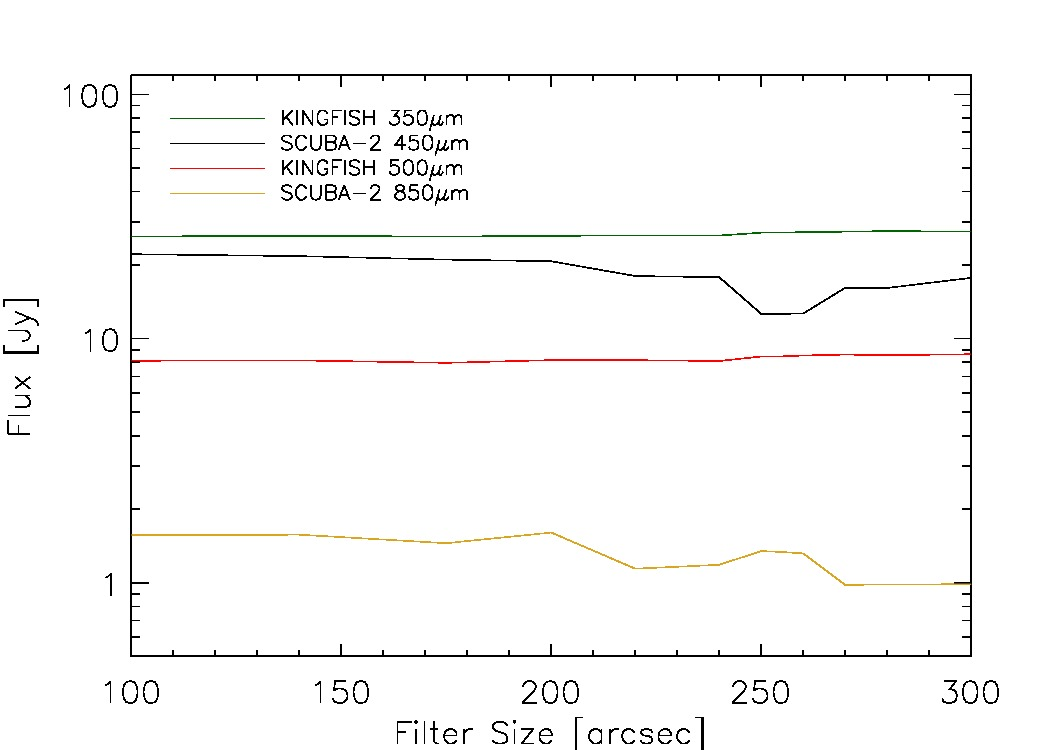
\includegraphics[scale=0.65]{obs_imgs/flux_line.jpeg}
  \caption[Flux Values vs  High-Pass Filter Sizes]{Returned flux values for NGC3627 with varying high-pass filter sizes.  The KINGFISH fluxes have been been processed using the fakesource process, $\S$\ref{fakesource_sec}}
  \label{filt_lines}
\end{figure}

\begin{figure}
  \centering
  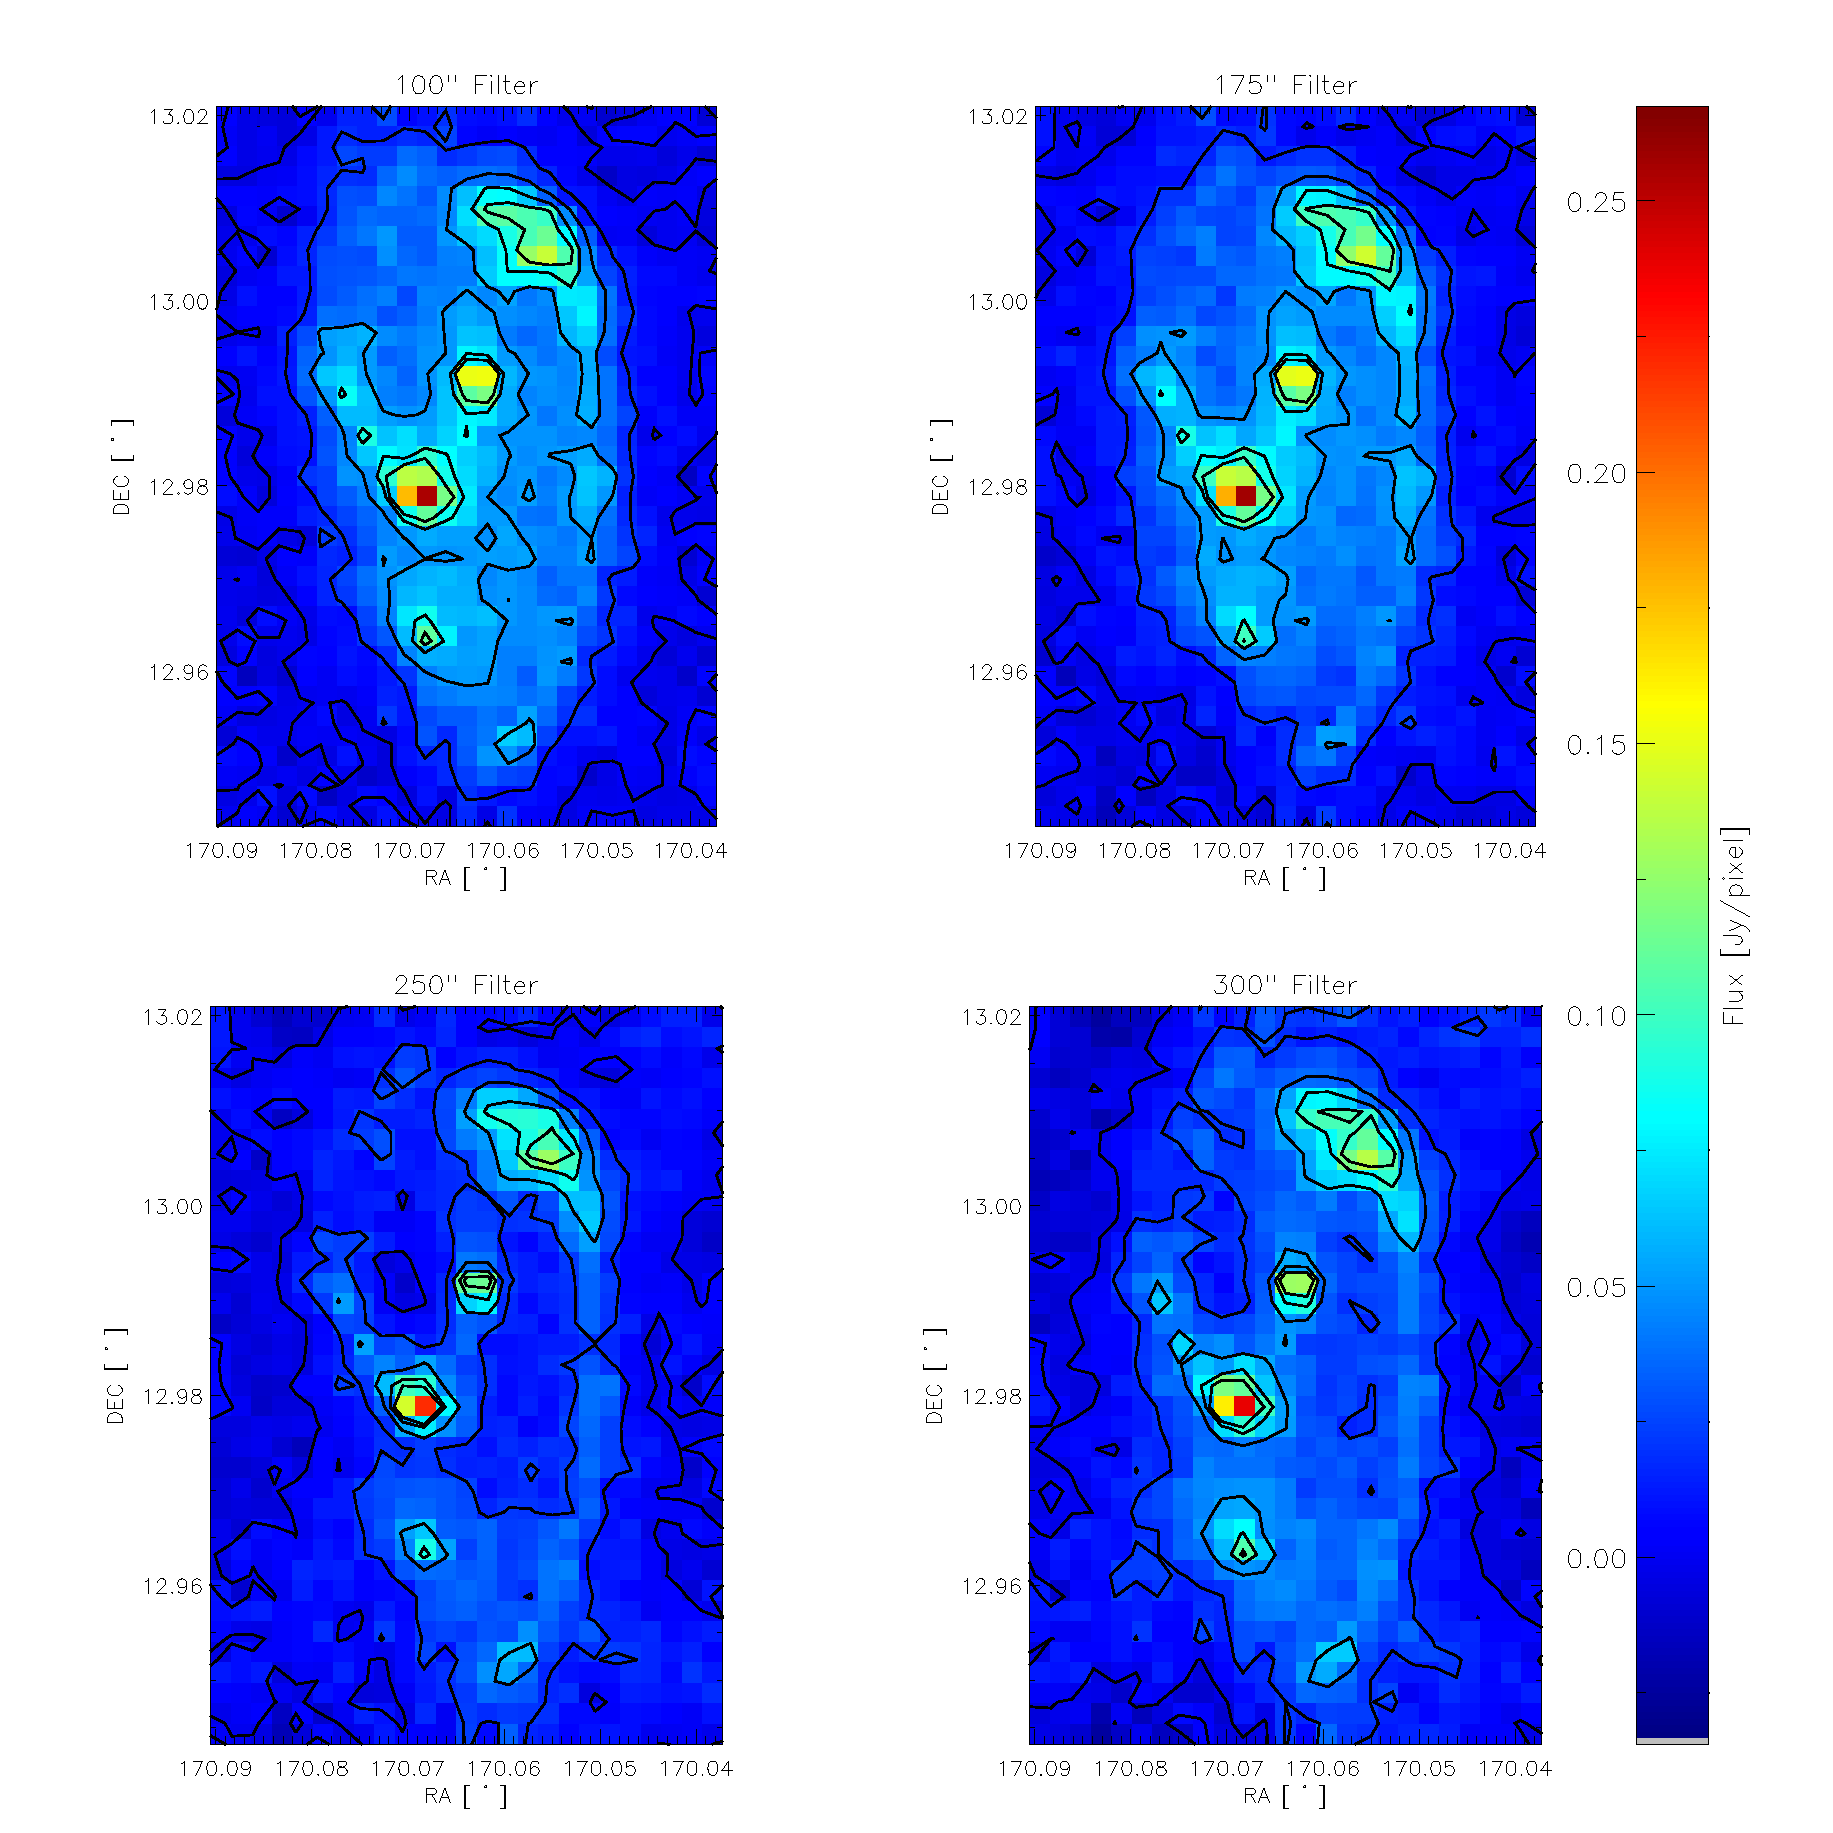
\includegraphics[scale=0.5]{obs_imgs/450_comparison_4.eps}
  \caption[450$\mu$m High-Pass Filter Images]{Four 450$\mu$m maps of NGC3627 using varying high-pass filter sizes.  The contours shown are for 0.0, 0.02, 0.05, 0.08 and 0.1 Jy/pixel for each image with 8$\arcsec$ by 8$\arcsec$ pixels.}
    \label{450_flt}
\end{figure}

\begin{figure}
  \centering
  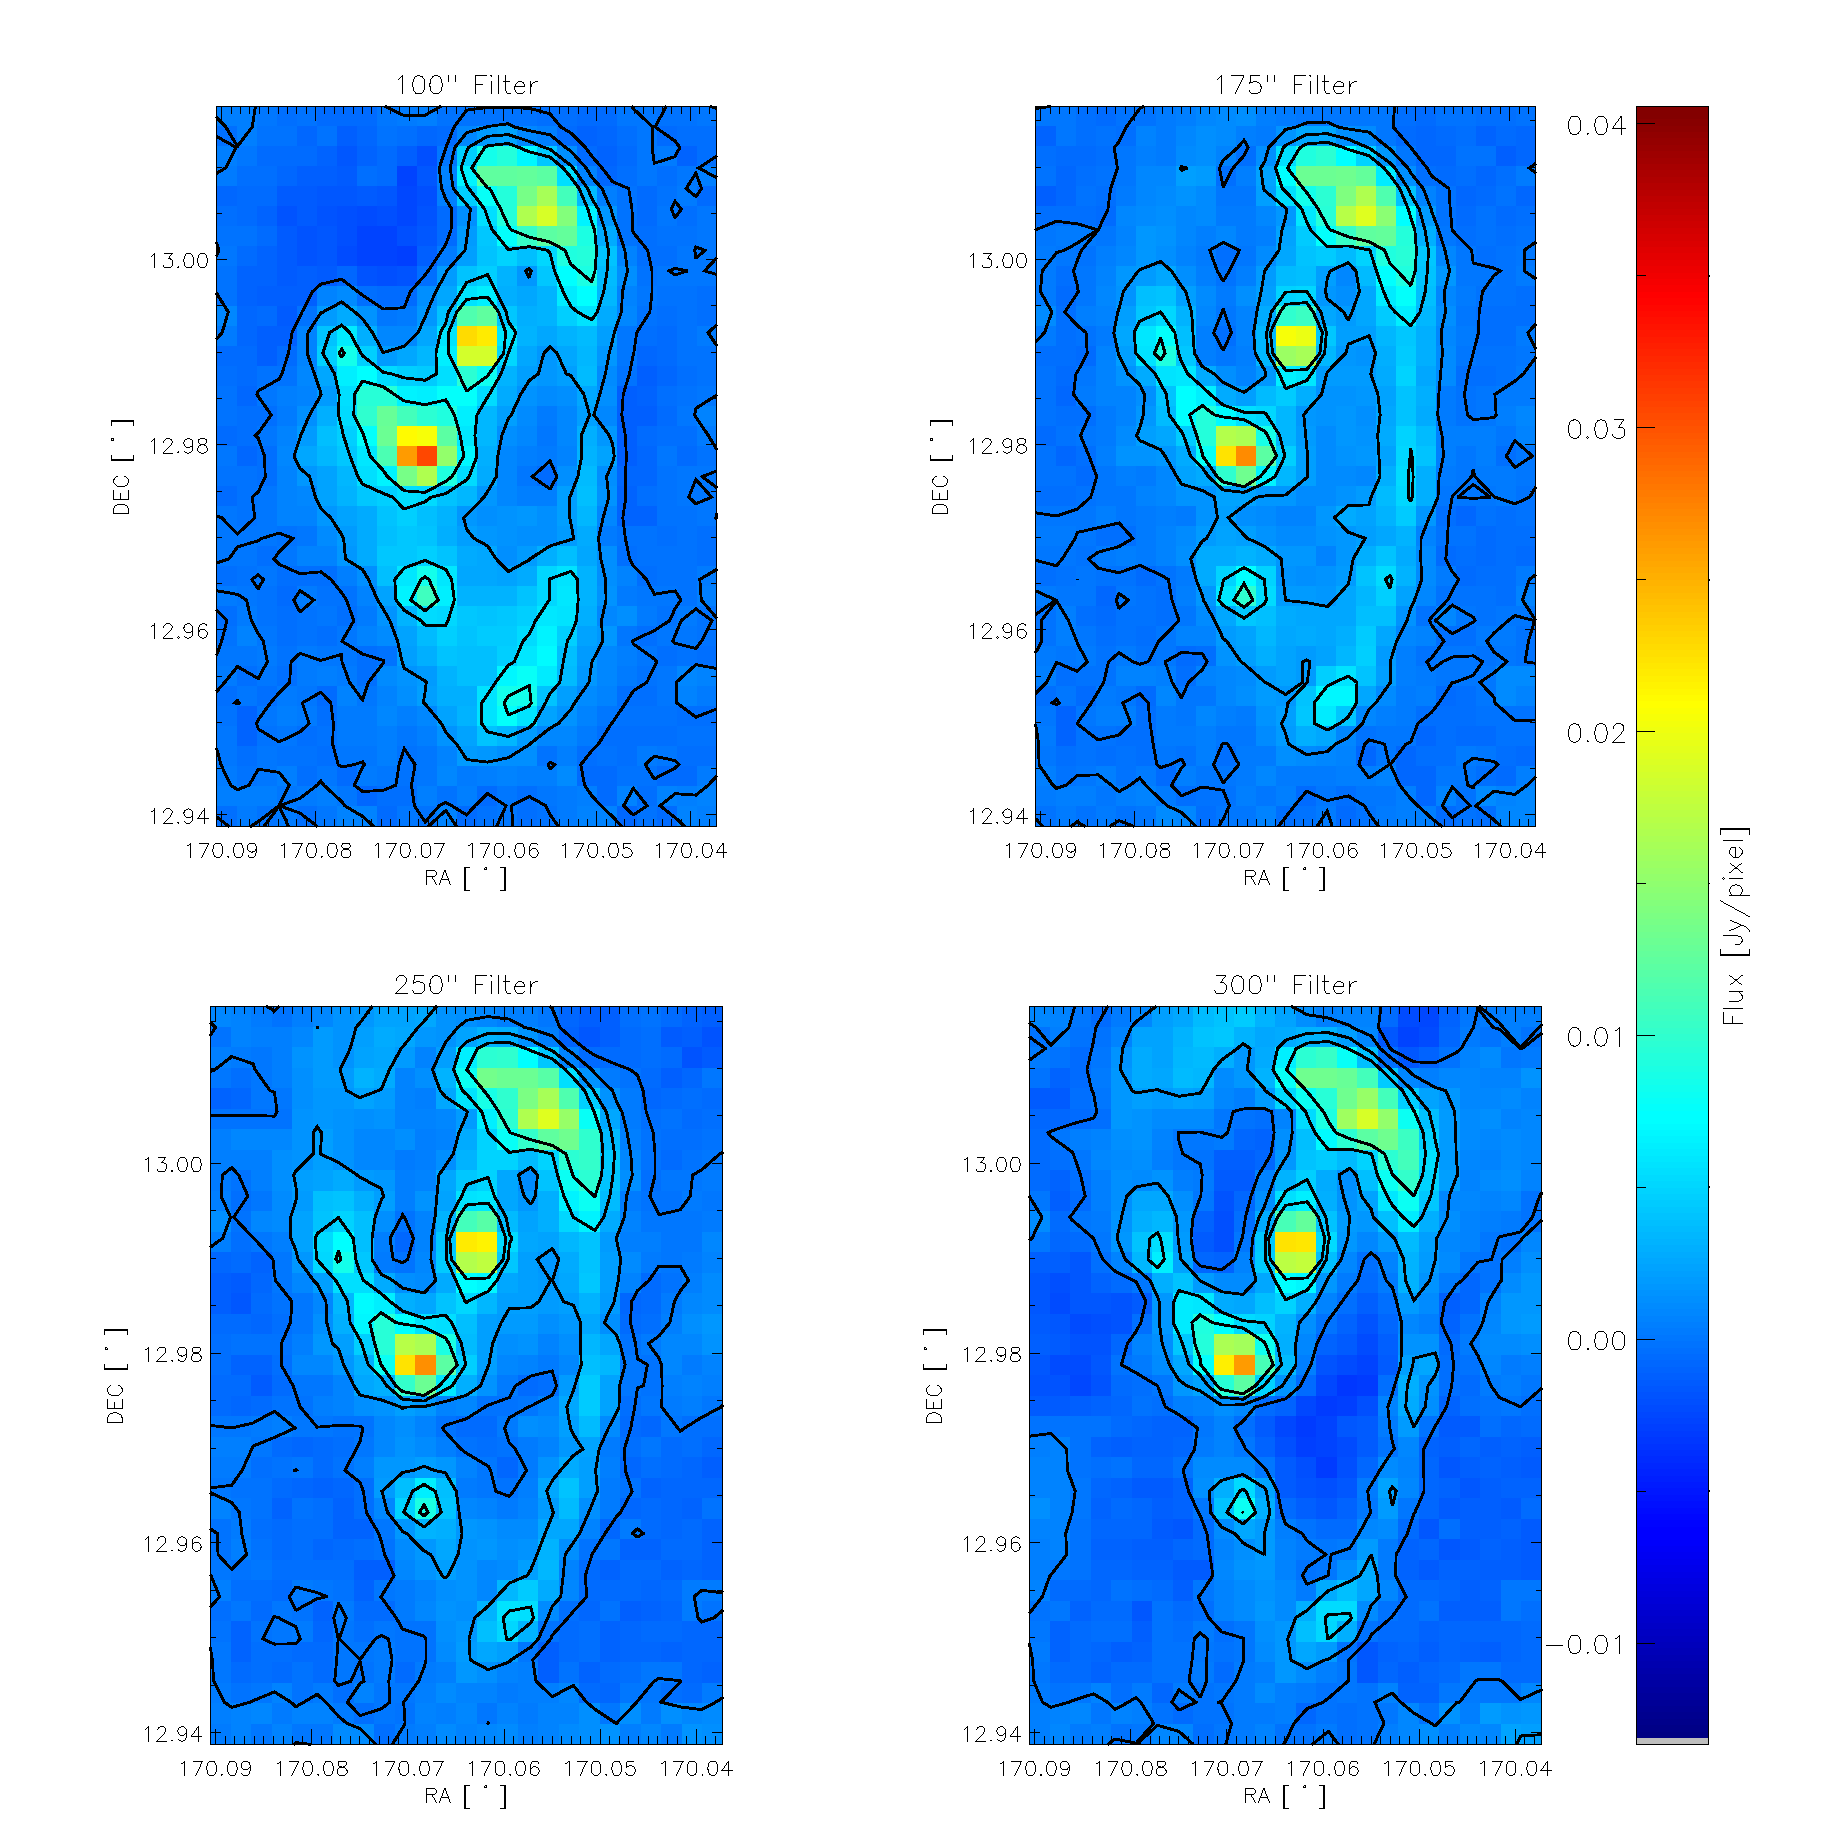
\includegraphics[scale=0.5]{obs_imgs/850_comparison_4.eps}
  \caption[850$\mu$m High-Pass Filter Images]{Four 850$\mu$m maps of NGC3627 using varying high-pass filter sizes.  The contours shown are for 0.0, 0.002, 0.005, and 0.008 Jy/pixel for each image with 8$\arcsec$ by 8$\arcsec$ pixels.}
    \label{850_flt}
\end{figure}

The final 450$\mu$m image was then re-gridded down to a 4$\arcsec$ by 4$\arcsec$ pixel grid, and flux calibration values of 491000 and 4710 \citep{dempsey2013} were applied to convert from pW to mJy/beam and mJy/square arcsecond, respectively.  The 850$\mu$m maps were re-gridded to an 8$\arcsec$ by 8$\arcsec$ pixel size and used flux calibration values of 537000 and 2340 for mJy/beam and mJy/square arcsecond \citep{dempsey2013}.  The 4$\arcsec$ and 8$\arcsec$ pixels correspond to a 180pc and 360pc size scale for our target, NGC3627.  To simplify the analysis, the images are also converted to Jy/pixel.  The 450$\mu$m and 850$\mu$m images are shown in Figures \ref{fig_450} and \ref{fig_850}.  The calibration values used are the default flux calibration factors that are determined from our calibrator source, Uranus, in  \citep{dempsey2013}.  The overall noise in the final image can be seen in Table \ref{tab_obs_scuba2}.

\begin{figure}
  \centering
  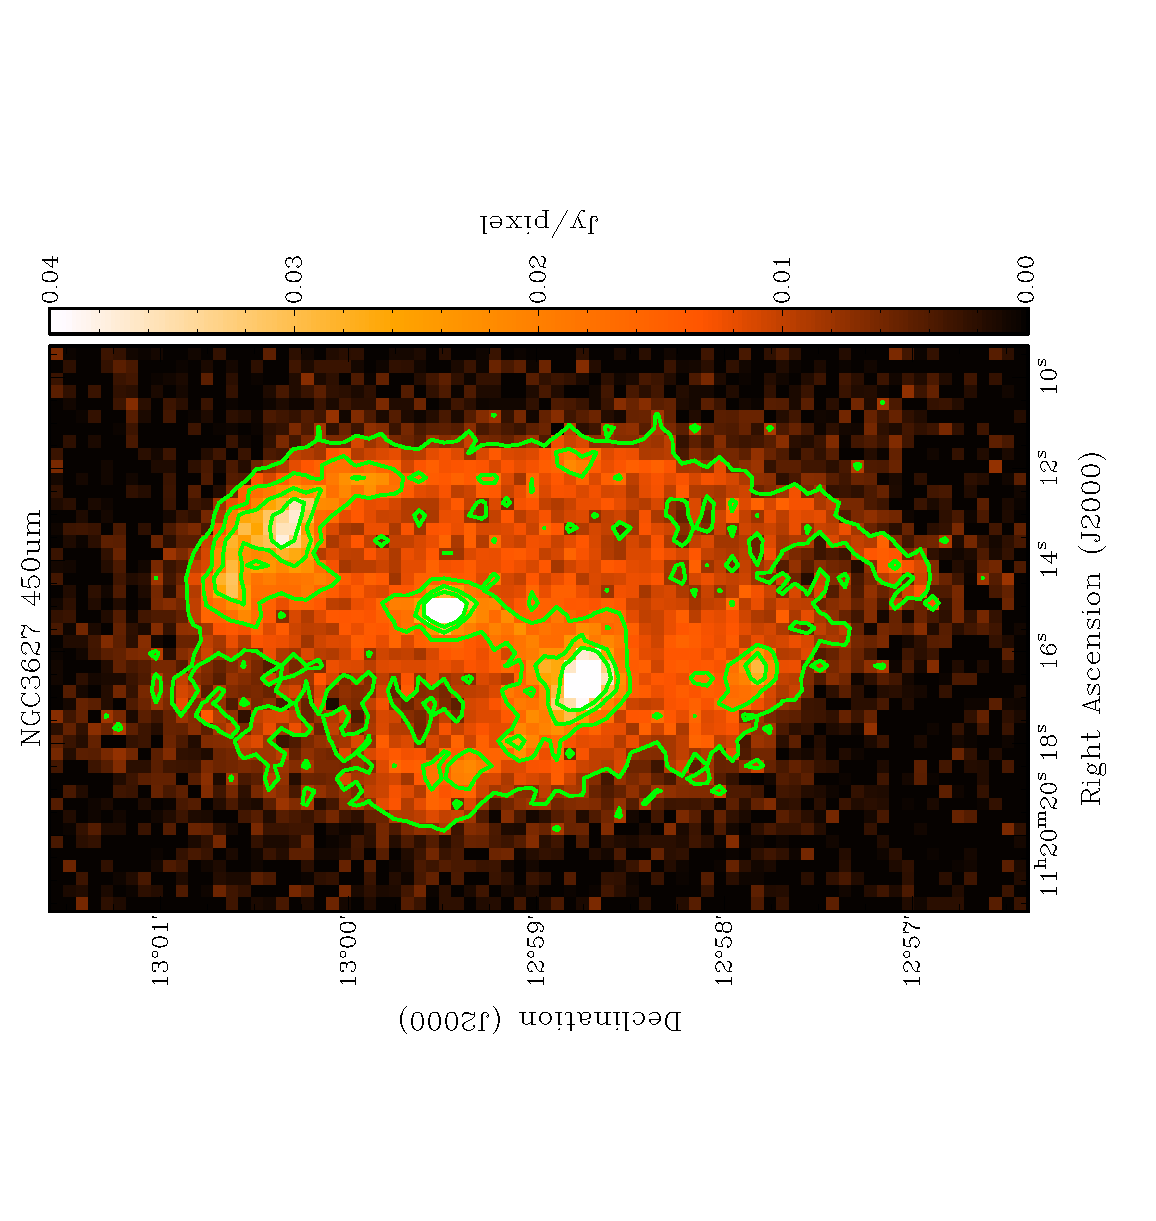
\includegraphics[width=1.\textwidth,angle=270]{obs_imgs/450_um.eps}
  \caption[NGC3627 450$\mu$m Observations]{450$\mu$m observation produced at the end of the image production with 20\%, 40\%, 60\%, and 80\% contours with 4$\arcsec$ by 4$\arcsec$ pixels.}
    \label{fig_450}
\end{figure}

\begin{figure}
  \centering
  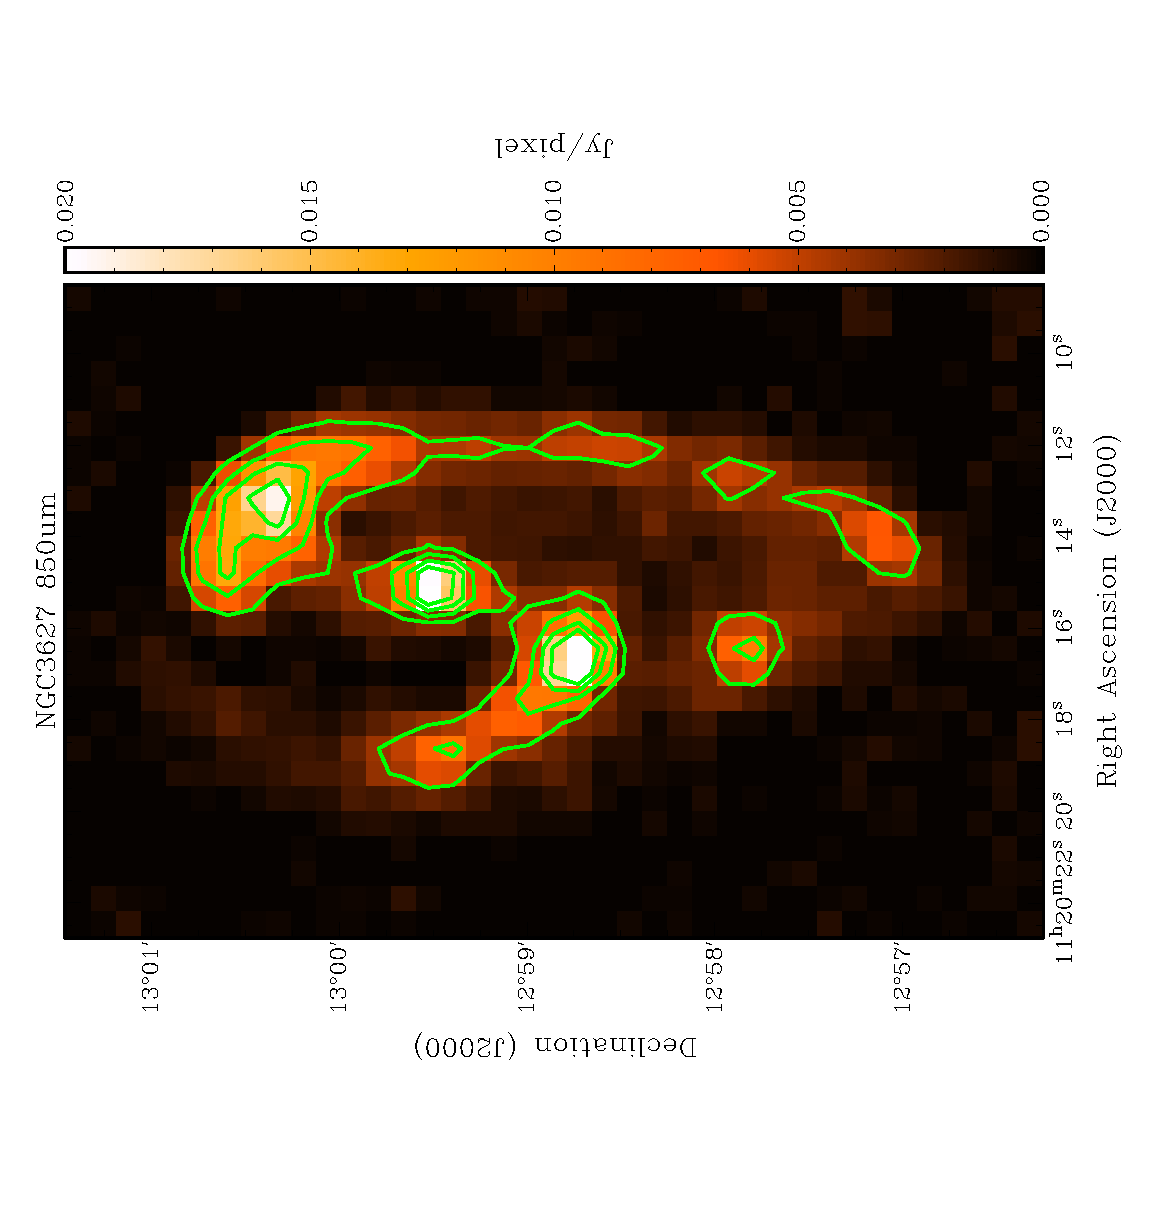
\includegraphics[width=1.\textwidth,angle=270]{obs_imgs/850_um.eps}
  \caption[NGC3627 850$\mu$m Observations]{850$\mu$m observation produced at the end of the image production with 20\%, 40\%, 60\%, and 80\% contours with 8$\arcsec$ by 8$\arcsec$ pixels.}
    \label{fig_850}
\end{figure}

\begin{deluxetable}{cccccc}
  \tabletypesize{\footnotesize}
  \tablecolumns{6}
  \tablewidth{0pt}
  \tablecaption{Properties of NGC3627 SCUBA-2 Observations\label{tab_obs_scuba2}}
  \tablehead{\colhead{Observation} & \multicolumn{4}{c}{Beam Properties} & \colhead{RMS} \\
& $\alpha$ & $\theta_{\alpha}$ & $\beta$ & $\theta_{\beta}$ & \it{[mJy / Pixel]}}
  \startdata
    450$\mu$m & 0.854 $\pm$ 0.002 & 7.48$\arcsec$ $\pm$ 0.03$\arcsec$ & 0.146 $\pm$ 0.003 & 23.1$\arcsec$ $\pm$ 0.2$\arcsec$ & 3.42  \\
    850$\mu$m & 0.9624 $\pm$ 0.0002 & 12.8$\arcsec$ $\pm$ 0.004$\arcsec$ & 0.0376 $\pm$ 0.0002 & 44.5$\arcsec$ $\pm$ 0.09$\arcsec$ &  0.476 \\
   \enddata
\end{deluxetable}

\subsection{Beam Shape of the 450$\mu$m and 850$\mu$m Data} \\
The Uranus calibration images were used to determine the shape of the beam for the 450$\mu$m and 850$\mu$m observations.  The beam shape of both the 450$\mu$m and 850$\mu$m maps deviates from a single gaussian due to the second maximum of the airy diffraction pattern in the response function of the telescope and minor imperfections in the mirror of the JCMT due to boundaries of the panels \citep{dempsey2013}.  This abnormality is best represented by a sum of two gaussians whose amplitudes sum to unity \citep{dempsey2013}.  The average beam resolution for the 450$\mu$m and 850$\mu$m data are reported in Table \ref{tab_obs_scuba2} and within an acceptable difference from the values found in \cite{dempsey2013}.  The calibration images, fitted beams, and the residual of the fits can be seen in Figure \ref{fig_calib}.  The residuals seen in here are due to asymmetries in the Uranus PSF.  The contribution of the error beam in the 850$\mu$m emission is negligible, and allows the beam to be approximated by a single gaussian.  However, the contribution of the error beam in the 450$\mu$m images was large enough to require special treatment in order to properly match the beams for analysis.

\begin{figure}
  \centering
  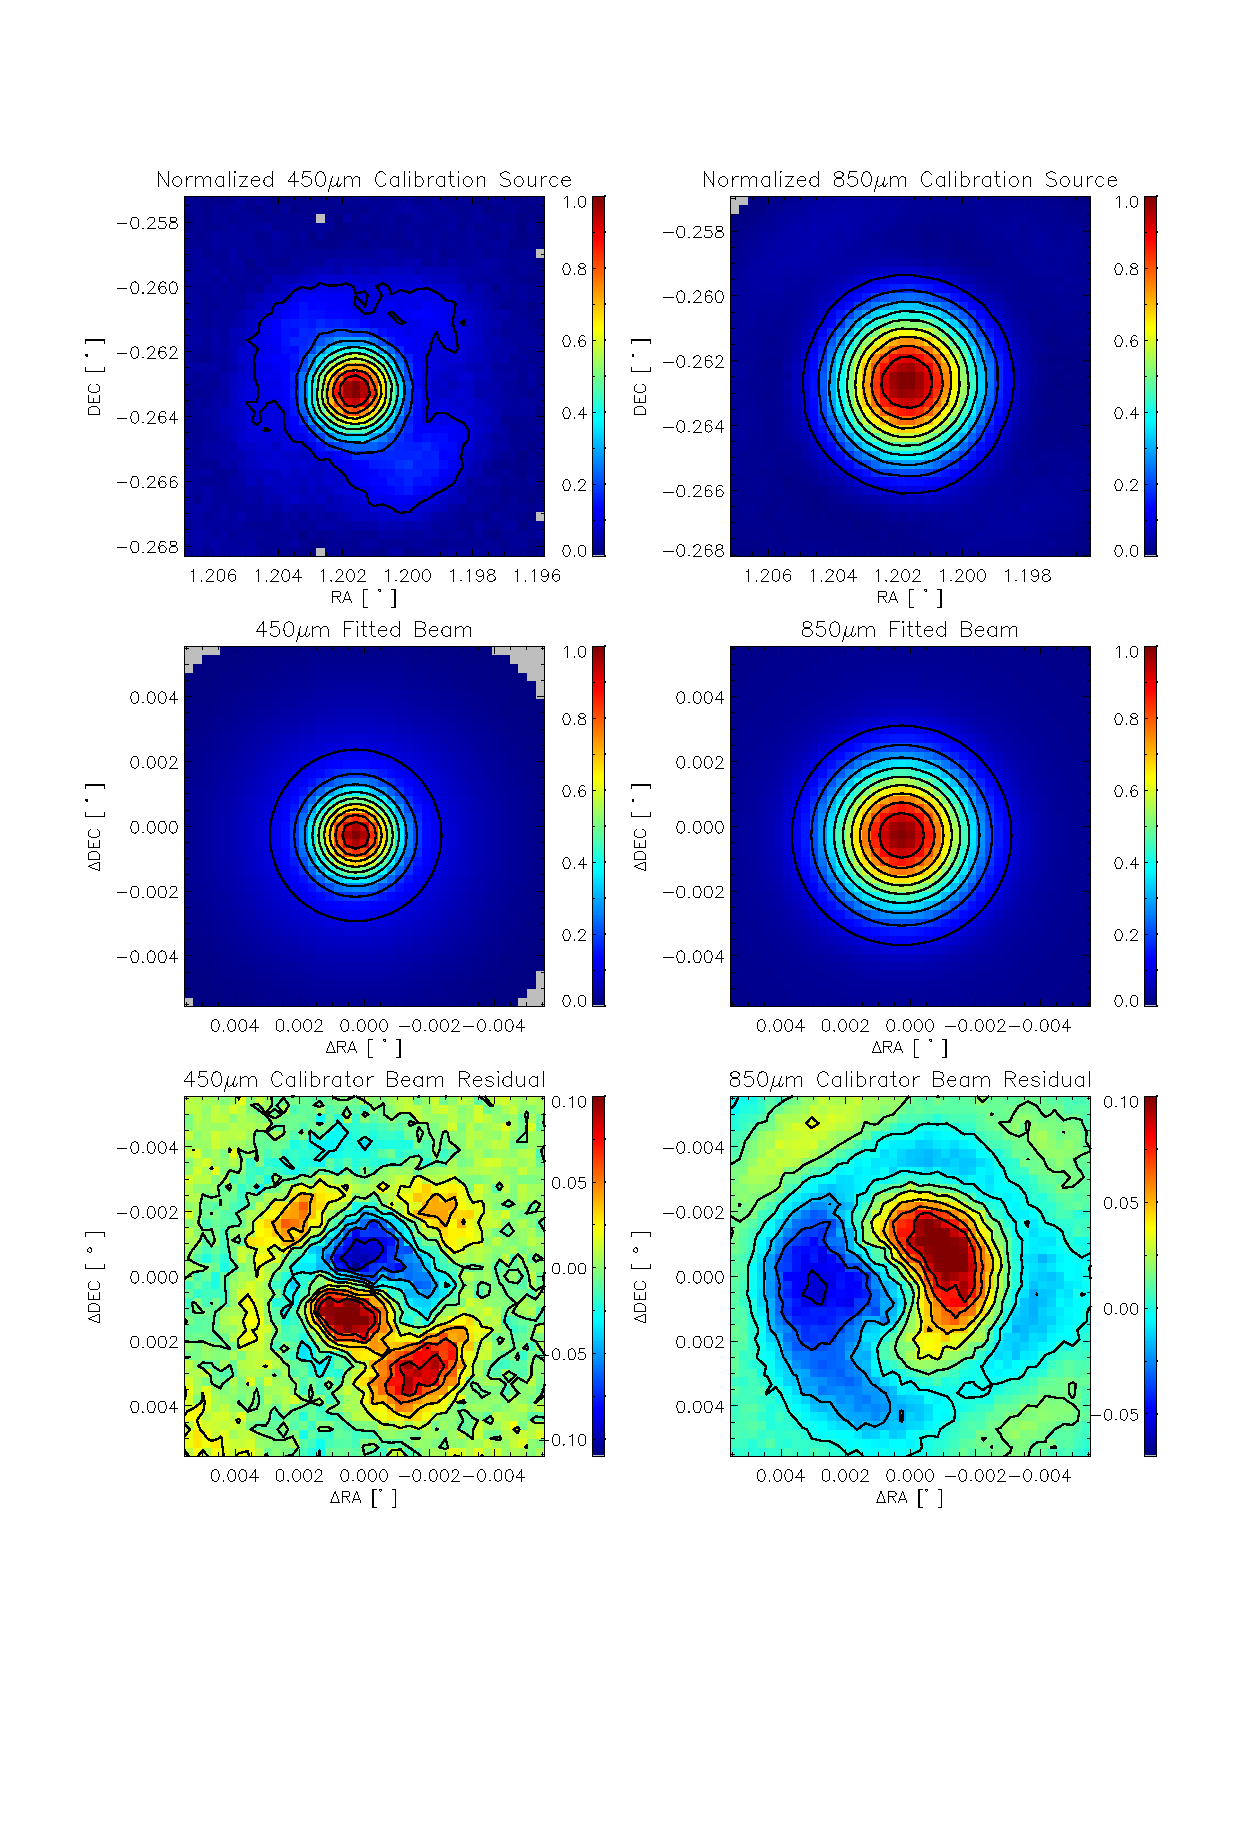
\includegraphics[width=1.\textwidth, trim={0 5cm 0 0}]{obs_imgs/calib_beams.eps}
  \caption[SCUBA-2 Calibration and Beams]{The top row shows the Uranus images taken on January, 8th 2012 for 450$\mu$m on the left and 850$\mu$m on the right.  The middle row shows the fitted beams for 450$\mu$m on the right and 850$\mu$m on the left using the double gaussian beam shape. The bottom row shows the difference between the original image and the fitted beam.  The contours in the image are from 10\% to 90\% in intervals of 10\%.}
    \label{fig_calib}
\end{figure}

\section{Ancillary Data}\label{ancillary}

The scientific goals of this thesis require data outside the capabilities of SCUBA-2.  For instance, accurately determining the dust mass involves fitting the spectral energy distribution (SED) for NGC3627.  To successfully fit an SED, we need shorter wavelength data to fully probe the cold component of this galaxy. We used data ranging from 100$\mu$m to 500$\mu$m from the KINGFISH survey \citep{kennicutt2011} to gain a large enough wavelength range for fitting the cold component.  Secondly, the bandpass of the 850$\mu$m filter contains the CO J=3-2 line.  In order to get a valid measurement of the dust mass, this contribution had to be removed.  We used emission data from the NGLS from the HARP instrument on the JCMT \citep{wilson2012} to remove this contamination.  When a dust mass was obtained, we used CO J=1-0 from the Nobeyama 45-m telescope \citep{kuno2007}, CO J=2-1 from HERACLES \citep{leroy2009}, and $HI$ observations from THINGS \citep{walter2008} to determine a reasonable molecular hydrogen mass to calculate a dust-to-gas ratio.  In the next sections we give some details for these ancillary data sets.

\subsection{Key Insights on Nearby Galaxies: a Far-Infrared Survey with Herschel (KINGFISH)}

The Key Insights on Nearby Galaxies: a Far-Infrared Survey with Herschel (KINGSFISH) was designed to be a follow up to the Spitzer Infrared Nearby Galaxies Survey (SINGS) \citep{kennicutt2003} with observations of the warm and cold component of dust emission using the increased resolution from Herschel \citep{kennicutt2011}.  The main science goals of the KINGFISH survey were to better understand the star formation processes that were shielded by dust, to make resolved studies of heating and cooling of the interstellar medium (ISM), and to build an inventory of how cold dust emission relates to other dust components in the ISM \citep{kennicutt2011}.  The survey consists of 61 nearby galaxies (d$<$30Mpc) that cover a range of environments.  Each target was observed at 70$\mu$m, 100$\mu$m, 160$\mu$m, 250$\mu$m, 350$\mu$m, and 500$\mu$m.  Our analyis focuses on fitting the cold component of NGC3627's SED, so we omitted the 70$\mu$m emission from the fitting, and processed the data through MAKEMAP as described below in $\S$ \ref{data_agree}.  The rms and beam size after the large scale structure has been removed can be seen in Table \ref{tab_obs_kfish} given for 8$\arcsec$ by 8$\arcsec$ pixels, while the preconvolved maps are shown in Figures \ref{fig_100} to \ref{fig_500}.

\begin{figure}
  \centering
  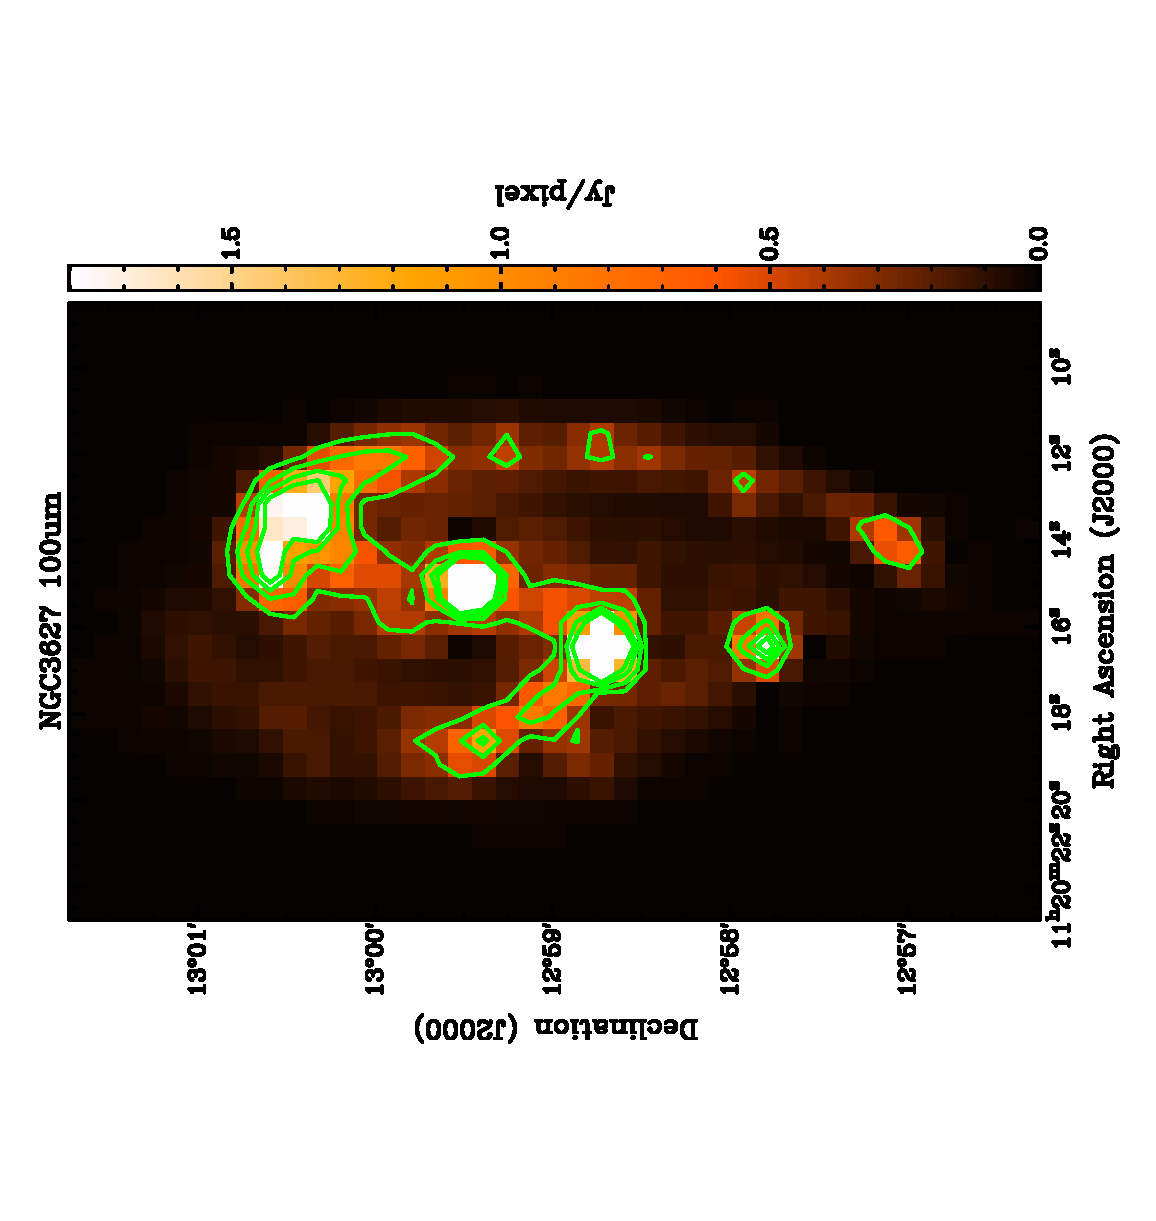
\includegraphics[width=1.\textwidth,angle=270]{obs_imgs/100_rem.eps}
  \caption[NGC3627 100$\mu$m Observations]{Image after the MAKEMAP filtering of 100$\mu$m observations with 20\%, 40\%, 60\%, and 80\% contours.}
  \label{fig_100}
\end{figure}

\begin{figure}
  \centering
  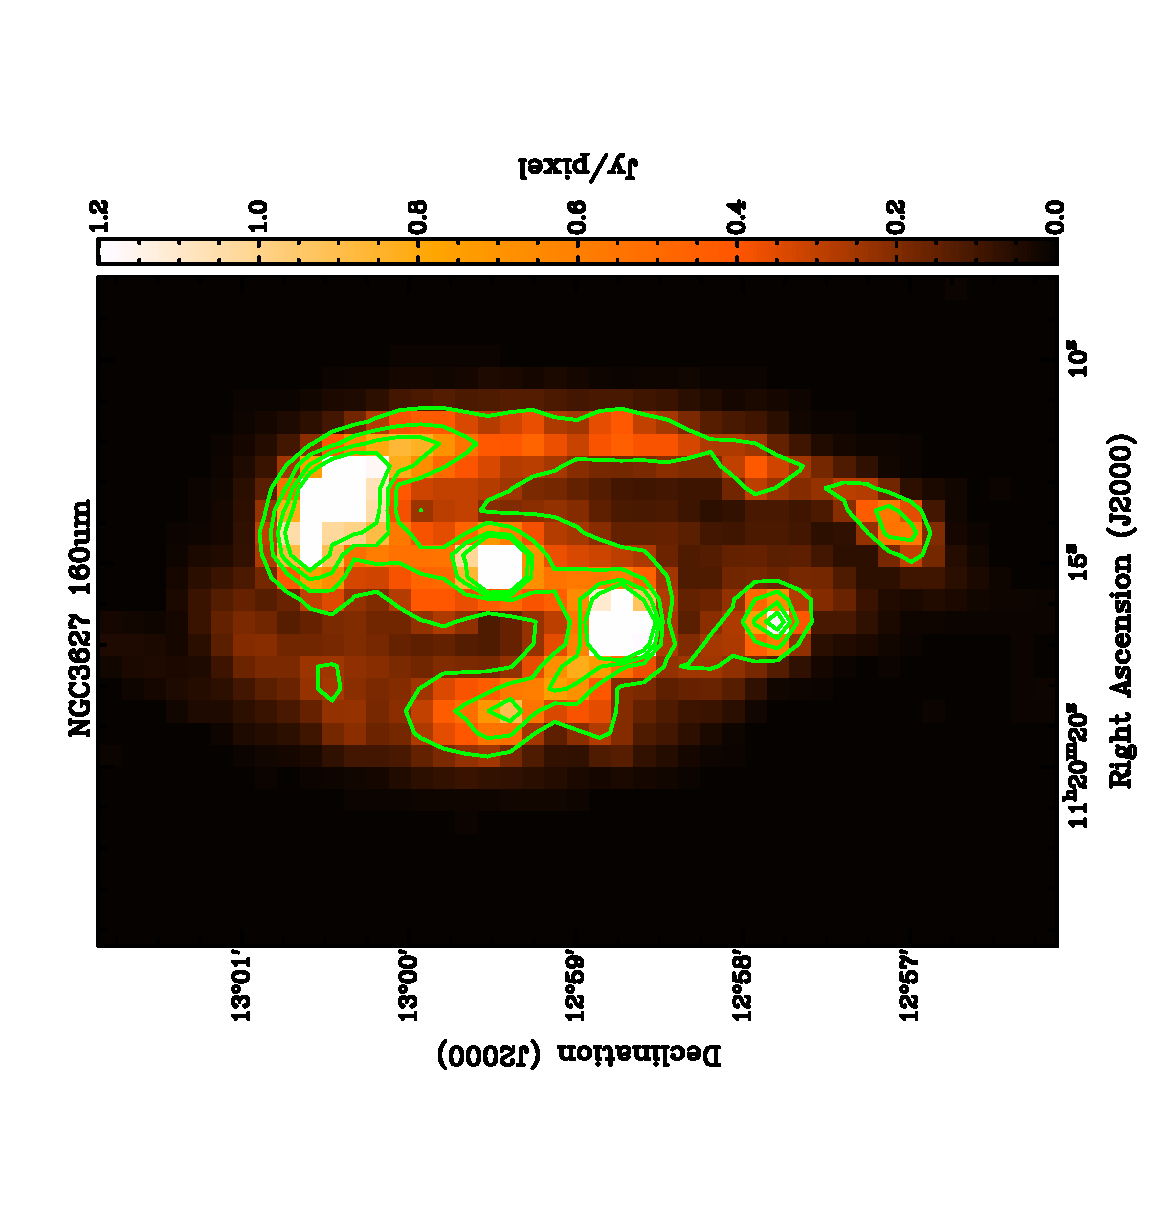
\includegraphics[width=1.\textwidth,angle=270]{obs_imgs/160_rem.eps}
  \caption[NGC3627 160$\mu$m Observations]{Image after the MAKEMAP filtering of 160$\mu$m observations with 20\%, 40\%, 60\%, and 80\% contours.}
  \label{fig_160}
\end{figure}

\begin{figure}
  \centering
  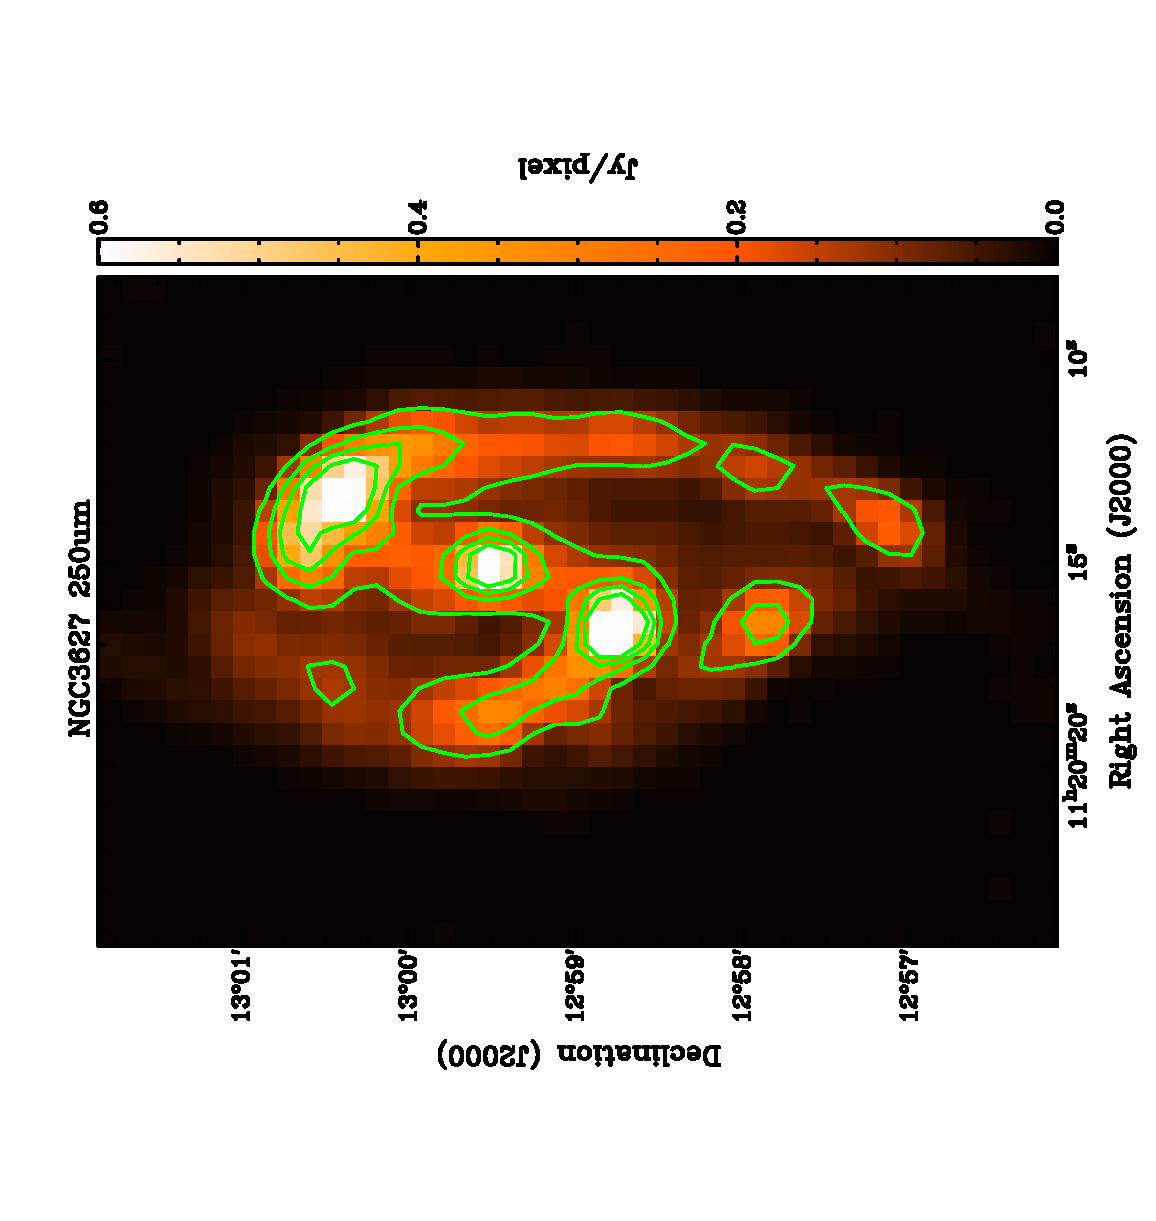
\includegraphics[width=1.\textwidth,angle=270]{obs_imgs/250_rem.eps}
  \caption[NGC3627 250$\mu$m Observations]{Image after the MAKEMAP filtering of 250$\mu$m observations with 20\%, 40\%, 60\%, and 80\% contours.}
  \label{fig_250}
\end{figure}

\begin{figure}
  \centering
  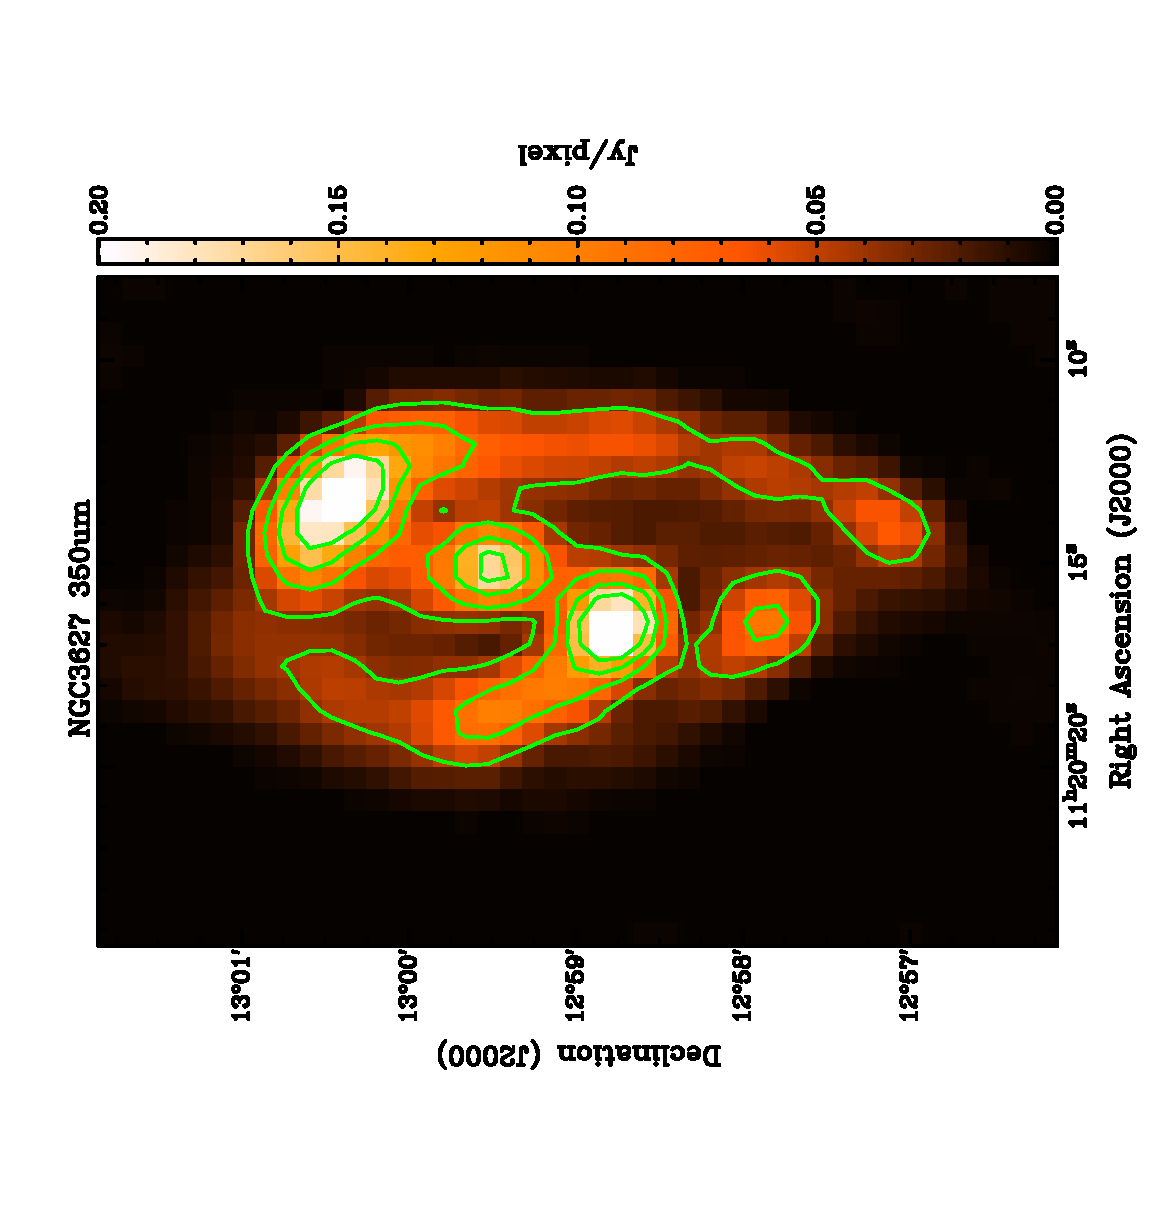
\includegraphics[width=1.\textwidth,angle=270]{obs_imgs/350_rem.eps}
  \caption[NGC3627 350$\mu$m Observations]{Image after the MAKEMAP filtering of the 350$\mu$m observations with 20\%, 40\%, 60\%, and 80\% contours.}
  \label{fig_350}
\end{figure}

\begin{figure}
  \centering
  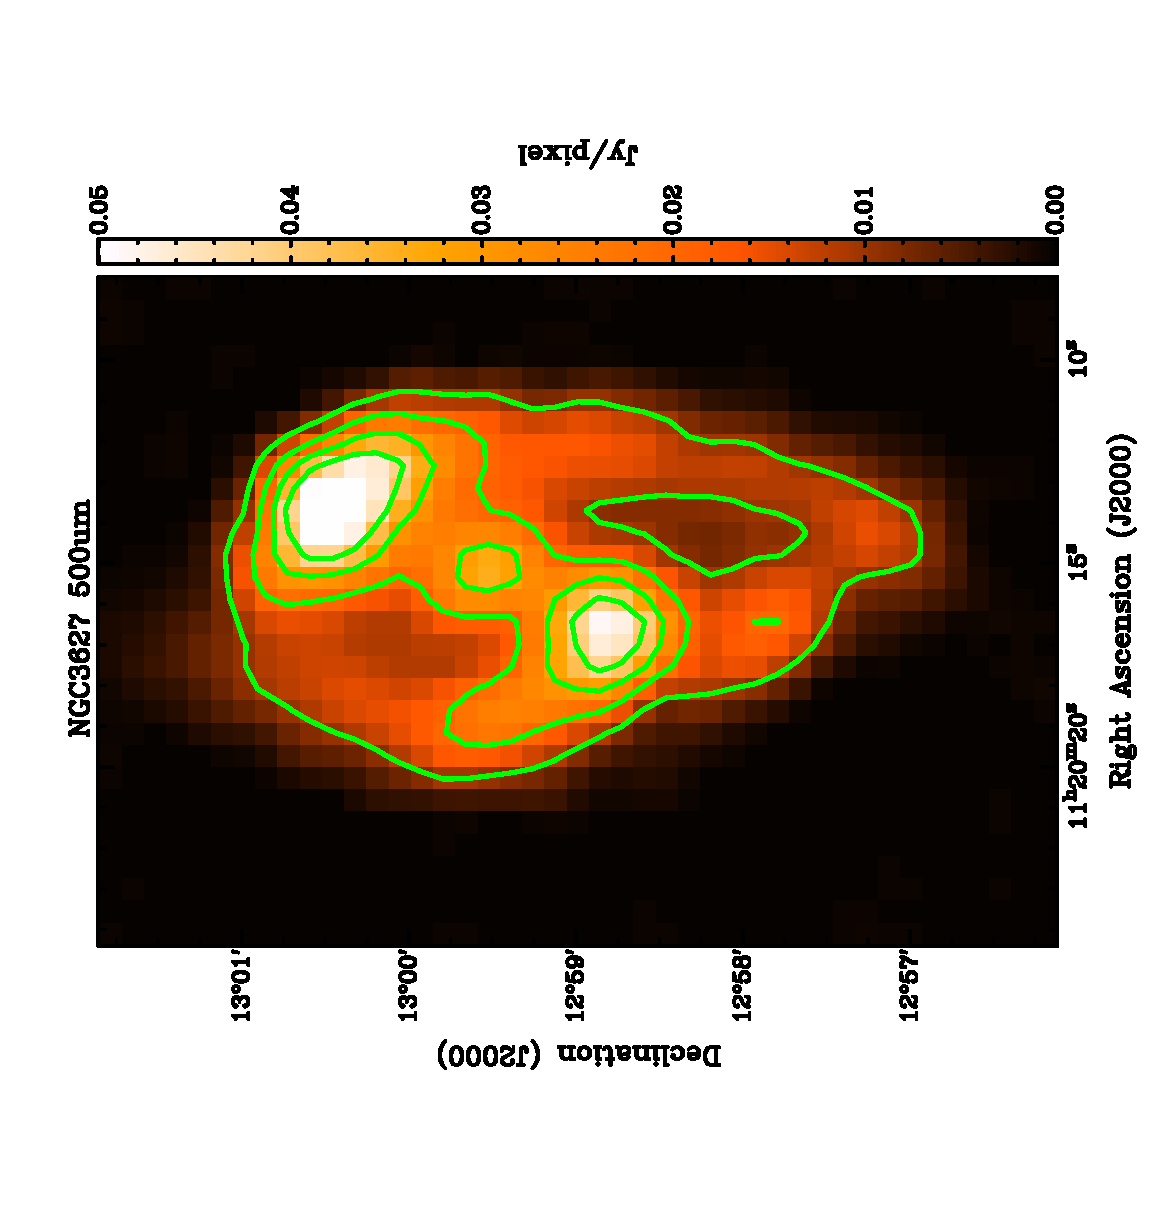
\includegraphics[width=1.\textwidth,angle=270]{obs_imgs/500_rem.eps}
  \caption[NGC3627 500$\mu$m Observations]{Image after the MAKEMAP filtering of the 500$\mu$m observations with 20\%, 40\%, 60\%, and 80\% contours.}
  \label{fig_500}
\end{figure}

\begin{deluxetable}{cccc}
%  \table{\footnotesize}
  \tablecolumns{4}
  \tablewidth{0pt}
  \tablecaption{Properties of NGC3627 KINGFISH Observations\label{tab_obs_kfish}}
  \tablehead{\colhead{Observation} & \colhead{Beam Properties } & \colhead{RMS} & \colhead{Percentage of Emission Removed} \\
 & $\theta_{beam}$ & \it{[mJy/Pixel]}}
  \startdata
    100$\mu$m & 6.8$\arcsec$ & 2.24 & 11\% \\
    160$\mu$m & 11.6$\arcsec$ & 3.95 & 17\% \\
    250$\mu$m & 18.0$\arcsec$ & 2.47 & 20\% \\
    350$\mu$m & 24.9$\arcsec$ & 1.08 & 21\% \\
    500$\mu$m & 36.0$\arcsec$ & 0.387 & 28\% \\
  \enddata
\end{deluxetable}

\subsection{Nearby Galaxies Legacy Survey (NGLS)}

The Nearby Galaxies Legacy Survey is an HI-selected set of 155 galaxies contained in the annulus of $2Mpc\leq d \leq25Mpc$ observed using the instrumentation on the JCMT \citep{wilson2012}.  The NGLS consists of data observed in several wavelengths that include the 450$\mu$m and 850$\mu$m data used for this thesis.  As mentioned previously, the bandpass for SCUBA-2's 850$\mu$m emission contains the CO J=3-2 line which is contained in the NGLS data set.  We used the zeroth moment CO J=3-2 maps from the NGLS to determine the percentage of CO J=3-2 emission present in the 850$\mu$m band as well as removing it for an accurate SED analysis.  The rms and resolution of the CO J=3-2 emission are shown in Table \ref{tab_obs_NGLS} for 8$\arcsec$ by 8 $\arcsec$ pixels, and the scan prior to convolution is shown in Figure \ref{fig_co32}.

\begin{figure}
  \centering
  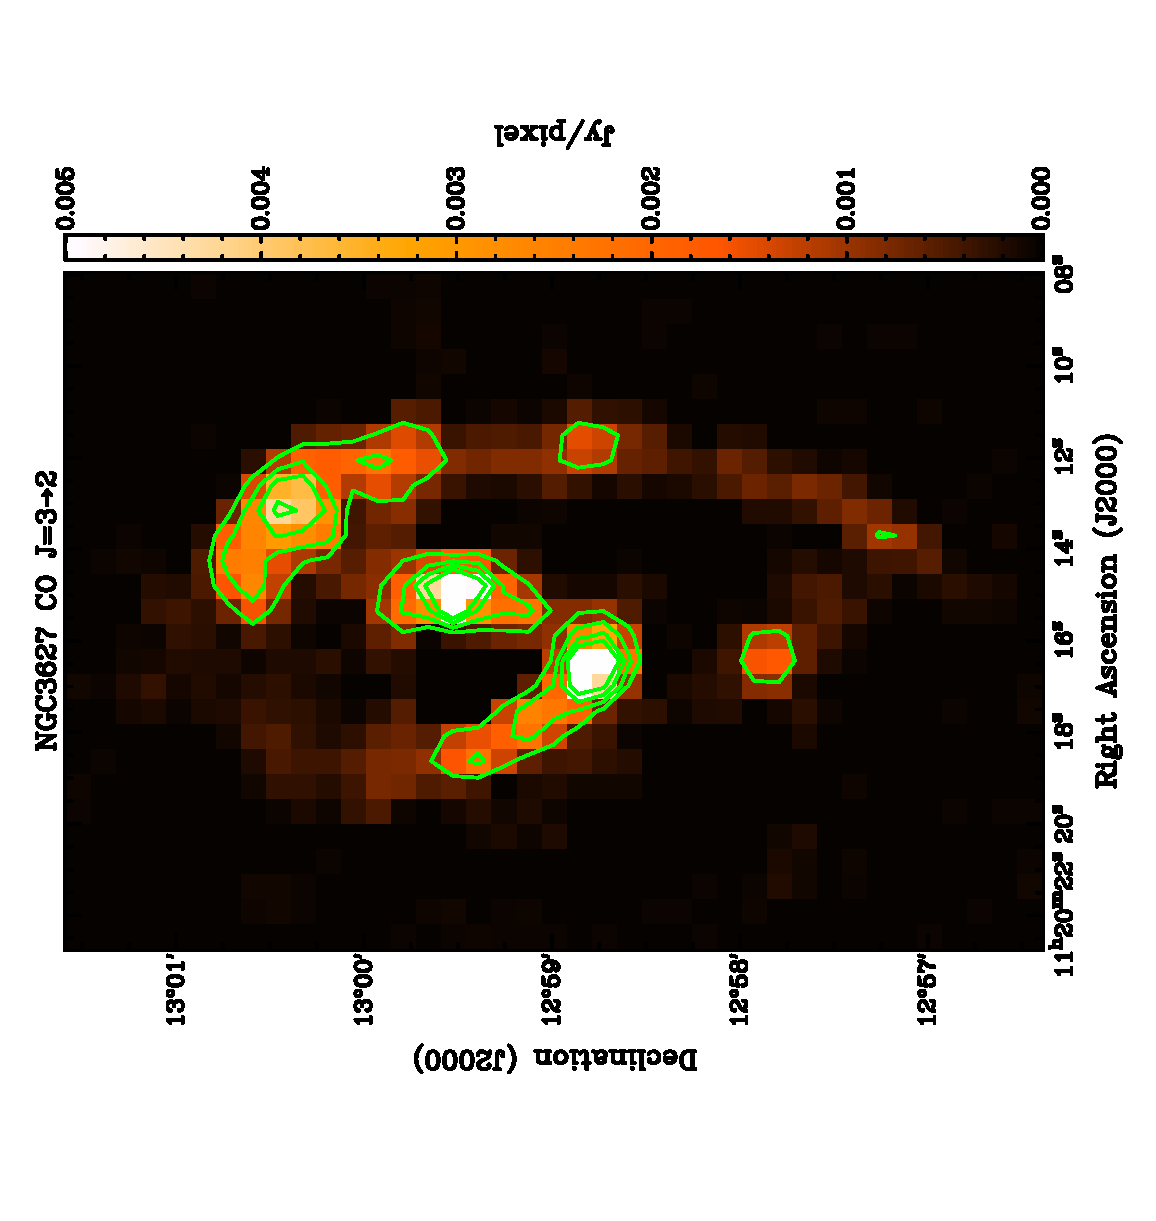
\includegraphics[width=1.\textwidth, angle=270]{obs_imgs/32_rem.eps}
  \caption[NGC3627 CO J=3-2 Observations]{Residual of the MAKEMAP filtering of CO J=3-2 observations used to subtract line contamination from 850$\mu$m SCUBA-2 map with 20\%, 40\%, 60\%, and 80\% contours.}
  \label{fig_co32}
\end{figure}

\begin{deluxetable}{cccc}
  \tablecolumns{4}
  \tablewidth{0pt}
  \tablecaption{Properties of NGC3627 NGLS Observations\label{tab_obs_NGLS}}
  \tablehead{\colhead{Observation} & \colhead{Beam Properties } & \colhead{RMS} & \colhead{Percentage of Emission Removed} \\
 & $\theta_{beam}$ & \it{[mJy/Pixel]}}
  \startdata
    CO J=3-2 & 14.5$\arcsec$ & 1.28e-2& 29.8\% \\
  \enddata
\end{deluxetable}

%insert co32 img

\subsection{Nobeyama 45-m}\label{nob_sec}

Determining a dust-to-gas ratio requires a molecular tracer to estimate the amount of molecular hydrogen present.  The most frequently used tracer is CO J=1-0 due to its abundance in the ISM.  The CO J=1-0 data we used was taken from the Nobeyama 45-m CO Atlas of Nearby Spiral Galaxies observed to better understand the role of bars relating to molecular gas \citep{kuno2007}.  The Nobeyama 45-m CO Atlas consists of galaxies with morphologies ranging from Sa to Scd, located less than 25Mpc from the Milky Way, inclination values less than $79^{\circ}$, 100$\mu$m flux greater than 10Jy, and spiral structure that has not been compromised through interactions.  Any galaxies that met these criteria were then observed with the Nobeyama 45-m telescope \citep{kuno2007}.  The beam sizes and rms of the filtered CO J=1-0 map are displayed in Table \ref{tab_obs_n45} for 8$\arcsec$ by 8$\arcsec$ pixels, and the final image product can be seen in Figure \ref{fig_co10}.

\begin{figure}
  \centering
  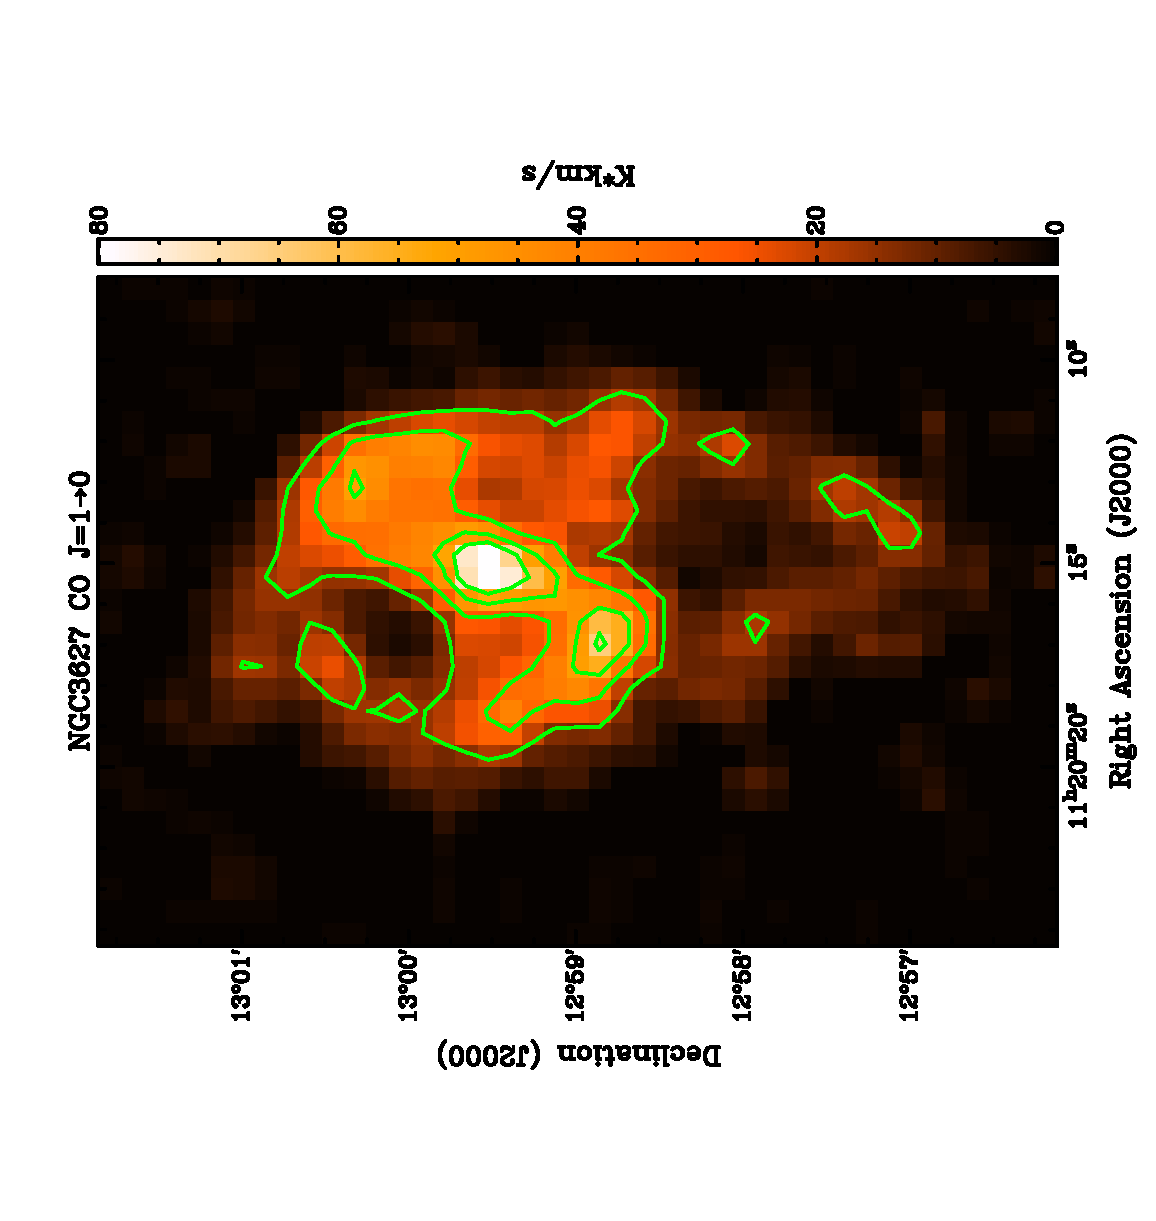
\includegraphics[width=1.\textwidth, angle=270]{obs_imgs/10_rem.eps}
  \caption[NGC3627 CO J=1-0 Observations]{Residual of the MAKEMAP filtering of CO J=1-0 observations with 20\%, 40\%, 60\%, and 80\% contours.}
  \label{fig_co10}
\end{figure}

\begin{deluxetable}{cccc}
  \tablecolumns{4}
  \tablewidth{0pt}
  \tablecaption{Properties of NGC3627 Nobeyama 45-m Observations\label{tab_obs_n45}}
  \tablehead{\colhead{Observation} & \colhead{Beam Properties } & \colhead{RMS} & \colhead{Percentage of Emission Removed} \\ 
  & $\theta_{beam}$ & \it{[K km/s]}}
  \startdata
    CO J=1-0 & 15.0$\arcsec$ & 0.681 & 20\% \\
  \enddata
\end{deluxetable}

\subsection{Hetrodyne Reciever Array CO-Line Extragalactic Survey (HERACLES)}

The CO J=2-1 line was used to determine a CO ${2-1} / {1-0}$ line ratio which can be used to trace a gradient in $\alpha_{CO}$ and hint towards regions of high star formation \citep{reuter1996}.  We used the CO J=1-0 data from the Nobeyama 45-m telescope ($\S$ \ref{nob_sec}), and CO J=2-1 from the Hetrodyne Reciever Array CO-Line Extragalactic Survey (HERACLES) using the IRAM 30-m telescope.  The main goal of HERACLES was to quantify the relationship between atomic and molecular gas and star formation using a large sample of galaxies \citep{leroy2009}.  The sample of galaxies chosen were targets contained in THINGS that were within the observing limits of the IRAM 30-m telescope.  The final CO J=2-1 image can be seen in Figure \ref{fig_co21} and the image properties can be seen in Table \ref{tab_obs_heracles} with 8$\arcsec$ by 8$\arcsec$ pixels.

\begin{figure}
  \centering

  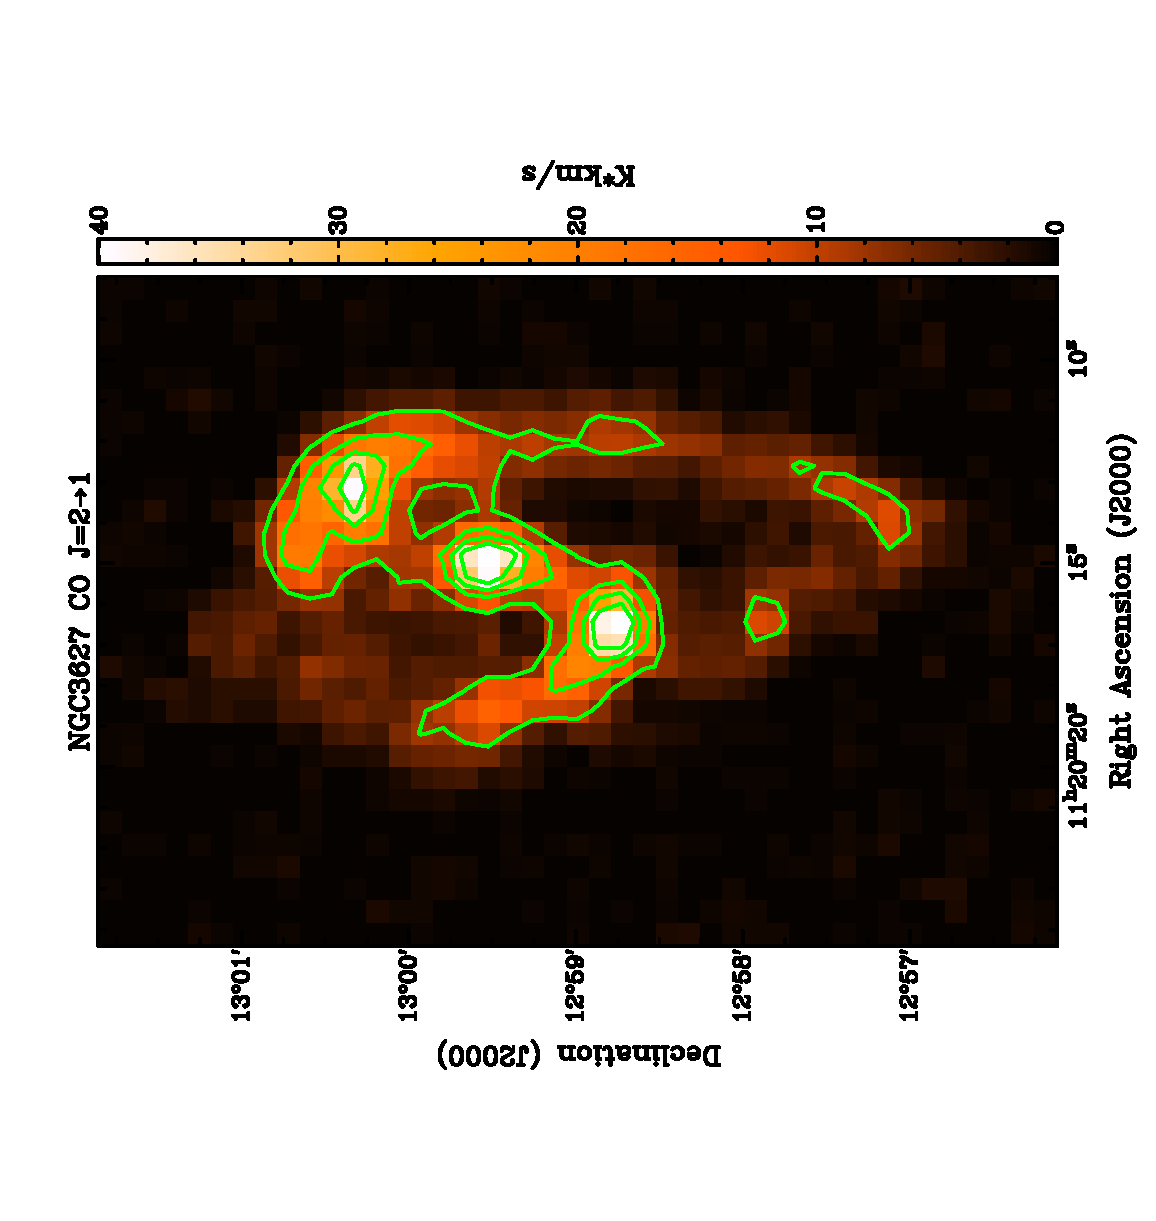
\includegraphics[width=1.\textwidth, angle=270]{obs_imgs/21_rem.eps}
  \caption[NGC3627 CO J=2-1 Observations]{Residual of the MAKEMAP filtering of CO J=2-1 observations with 20\%, 40\%, 60\%, and 80\% contours.}
  \label{fig_co21}
\end{figure}

\begin{deluxetable}{cccc}
  \tablecolumns{4}
  \tablewidth{0pt}
  \tablecaption{Properties of NGC3627 HERACLES Observations\label{tab_obs_heracles}}
  \tablehead{\colhead{Observation} & \colhead{Beam Properties } & \colhead{RMS} & \colhead{Percentage of Emission Removed} \\
  & $\theta_{beam}$ & \it{[K km/s]}}
  \startdata
    CO J=2-1 & 13.0$\arcsec$ & 0.305 & 7\% \\
  \enddata
\end{deluxetable}

\subsection{The HI Nearby Galaxy Survey (THINGS)}

To determine the gas-to-dust ratio we had to determine the total amount of gas present which includes both atomic and molecular hydrogen.  We approximated the amount of molecular hydrogen by using CO J=1-0, and measured the amount of atomic hydrogen (HI) present.  Our atomic hydrogen map came from The HI Nearby Galaxy Survey (THINGS) designed to observe HI emission in nearby galaxies with the extreme spatial resolution of the Very Large Array (VLA).  Targets in THINGS included many of the SINGS targets with the exception of known HI poor sources (E/S0 type galaxies), dynamically complex systems (edge-on spirals), and large extended galaxies found in the Local Group \citep{walter2008}.  The resolution and rms of the filtered image are shown in Table \ref{tab_obs_things} for 8$\arcsec$ by 8$\arcsec$ pixels.  The final data product is shown in Figure \ref{fig_HI} and has been converted to M$_\odot$ pc$^{-2}$ using 

\begin{equation}\label{eq:things_surf_den}
  M_{HI}\left[ M_\odot \right]=2.36 \times 10^5 D^2 \times \sum_{i}S_i\Delta v
\end{equation}

\noindent \citep{walter2008} and then dividing by the pixel area in pc$^2$ where D is the distance, and $\sum_{i}$S$_i\Delta$v is the first moment of the flux.  Since most of the HI emission is diffuse and extended, the filtering process resulted in a severe bowling lowering the surface densities, as well as removing a significant portion.

\begin{figure}
  \centering
  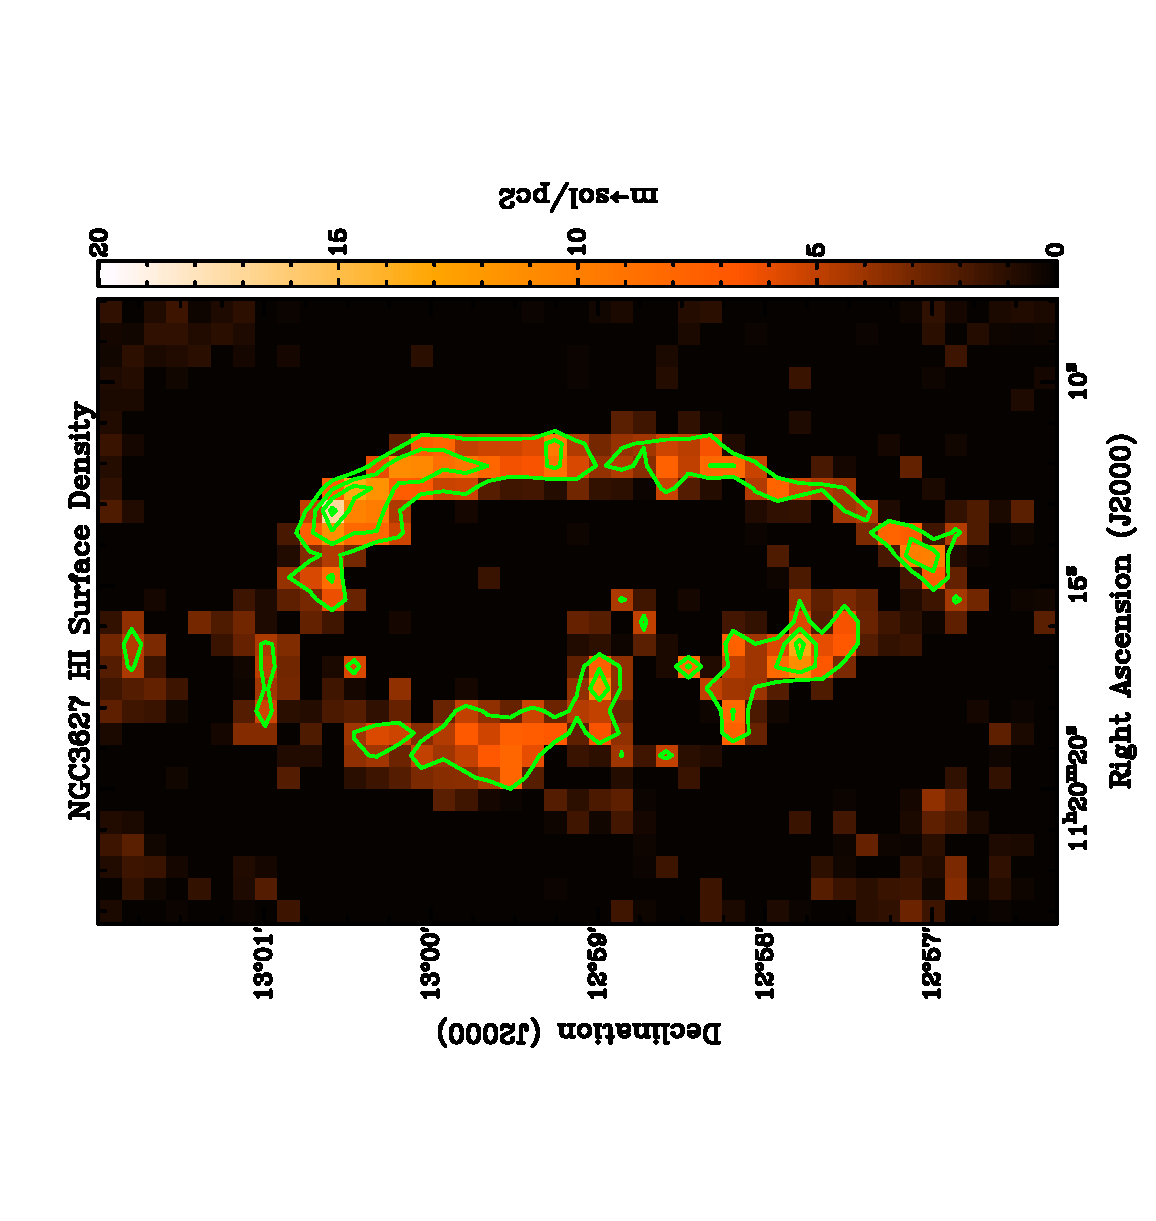
\includegraphics[width=1.\textwidth,angle=270]{obs_imgs/HI_rem.eps}
  \caption[NGC3627 HI Observations]{Residual of the MAKEMAP filtering of HI observations with 20\%, 40\%, 60\%, and 80\% contours.}
  \label{fig_HI}
\end{figure}

\begin{deluxetable}{cccccc}
  \tablecolumns{6}
  \tablewidth{0pt}
  \tablecaption{Properties of NGC3627 THINGS Observations\label{tab_obs_things}}
  \tablehead{\colhead{Observation} & \multicolumn{3}{c}{Beam Properties} & \colhead{RMS} & \colhead{Percentage of Surface Density Removed} \\
   & $\theta_{maj}$ & $\theta_{min}$ & $\theta_{PA}$ & \it{[$M_{\odot} / pc^2$]}}
  \startdata
    HI & 10.6$\arcsec$ & 8.85$\arcsec$ & -48.0$^\circ$ & 0.760 & $>$99\% \\  
  \enddata
\end{deluxetable}

\section{Data Preparation for Analysis}\label{data_agree}

Initially the data at the different wavelengths do not agree on several levels.  The differences consist of the presence of the large scale/extended structure and the different resolutions including the beam shape of the 450$\mu$m data.  We have taken several steps to correct for these disagreements and maximize the compatibility of the data.  In order to account for the varying beam resolutions, we use a gaussian convolution to increase the resolution of our maps to the largest beam size in our dataset, $\sigma_{max}$=36$\arcsec$.  An appropriate convolution beam width is determined by 

\begin{equation}\label{eq:gaus_kern}
  \sigma_{desire} = \sqrt{\sigma_{max}^2 - \sigma_{given}^2}
\end{equation}

\noindent where $\sigma_{desire}$ is the desired beam width, $\sigma_{max}$ is the beam size we are convolving to, and $\sigma_{given}$ is the beam size we are convolving from.  However, equation \ref{eq:gauss_kern} only works when the beams are well approximated by a single gaussian which is not the case for the 450$\mu$m beam.  The steps taken to match the resolution of the 450$\mu$m beam with the rest of the data set are given in $\S$\ref{450_fix_sec}.  

Removing any large scale structure from our ancillary data is implemented using a feature built into MAKEMAP that allows us to add fake sources into the data during production.  The fake source implementation allows us to remove the same amount of large scale structure from our ancillary data as was removed from the SCUBA-2 data.  The steps taken to prepare the ancillary data are described in $\S$\ref{fakesource_sec}.

%The largest difference in Ability of Herschell to observe submm unimpeded by atmo and the configuration setup of THIGNs allows for a bit of extended structure to arise in NGC3627.

\subsection{Accounting for the 450$\mu$m Error Beam}\label{450_fix_sec}

Taking the 450$\mu$m error beam into consideration is different than a normal beam convolution in the sense that we are not convolving the higher resolution map to the lowest resolution.  Instead we are adding in an error beam similar to the error beam found in the 450$\mu$m observations.  We have to take these steps because convolving a double gaussian beam with a single gaussian kernel will not sufficiently remove the error component of our beam resulting in a poor approximation to the wings of our beam shape.

In order to accommodate the 450$\mu$m map's error beam, we used a method employed by another SCUBA-2 legacy survey, the Gould Belt Survey.  This method uses the distributive nature of the Fourier transform to create similar error components in the beams we were convolving to and from.  Carrying out this convolution involves breaking the 450$\mu$m beam into its two components, $X_{\alpha}$ and $X_{\beta}$, to represent the main beam and error beam.  The values of the main beam amplitude, $X_\alpha$, and error beam amplitude, $X_\beta$, will sum to one so the height of the total beam is normalized to one.  The poorest resolution beam, $X_{max}$, is convolved with the two components $X_\alpha$ and $X_\beta$ and the resulting beams are added together.  This process produces an equivalent two component beam to the 450$\mu$m beam convolved with $X_{max}$.  The relationship can be expressed as 

\begin{equation} \label{eq_GBSmethod}
  \begin{split}
    X_{max} \ast X_{\alpha} + X_{max} \ast X_{\beta} & = \left(X_{\alpha} + X_{\beta}\right) \ast X_{max} \\
     & = X_{450\mu m} \ast X_{max}
   \end{split}
\end{equation}

\noindent where $X_{max}$ is the poorest resolution beam, $X_{\alpha}$ and $X_{\beta}$ are the main and error beam of the 450$\mu$m observations, and $X_{450\mu m}$ is the double gaussian beam shape of the 450$\mu$m observations.

\subsection{Extended Structure Removal via MAKEMAP}\label{fakesource_sec}

%adjusting the beam sizes to make the 450 beam work

%from the ancillary data set -- describes the fakesource stuff
Due to the combination of methods used in MAKEMAP, large scale/extended structure is removed from the final SCUBA-2 images.  However, in all of our ancillary data the large scale emission was present in the initial maps.  The removal of the extended features from our ancillary data was carried out by passing the data through MAKEMAP using a special function called fakemap.  Using fakemap allows us to pass an image though the SCUBA-2 processing and have it added into the image being processed.  We use the 850$\mu$m map as our base image for the filtering process and add the ancillary data to the 850$\mu$m image.  The output image then consists of the sum of the ancillary data and the 850$\mu$m map.  Finally, the ancillary data were isolated by subtracting the 850$\mu$m image from the fakemap output image.  

Preparing the data to be added via fakemap consists of either converting the images from their native units into pW using the 850$\mu$m flux calibration factor and scaling down to match the observed signal or by just applying a scaling factor.  Which method is used is based on the desired units of the final map, and can be separated by what purpose the data had in our analysis.

The data used in the SED fitting (KINGFISH and NGLS) were scaled to pW so they could have a similar reduction and calibration process as the SCUBA-2 maps.   The KINGFISH data are regridded to a 2$\arcsec$ by 2$\arcsec$ pixel size and have the appropriate calibration factor from \cite{dempsey2013} applied to convert from either MJy/sr to pW in the case of the 250$\mu$m, 350$\mu$m, and 500$\mu$m or from Jy/pixel to pW for the 100$\mu$m and 160$\mu$m.  Converting the CO J=3-2 data requires the final product to be in the same units as the 850$\mu$m observations in order to properly remove the molecular gas contribution.  Converting from K km/s to mJy/beam involvs applying a scaling constant of 0.70 [mJy/beam][K km/s]$^{-1}$ \citep{drabek2012} prior to applying the 850$\mu$m flux calibration factor to convert to pW.  

After the data has been converted to pW, the image used in fakemap is then scaled down to the same order of magnitude as the base image using a scaling factor specified prior to the map production.  After the fakemap image has been processed and the 850$\mu$m map subtracted, the maps are scaled back up using the same scaling factor used to scale them down and calibrated using the same flux calibration factors as the 850$\mu$m map and scaled to an 8$\arcsec$ by 8$\arcsec$ grid.  The amount of extended flux lost from the KINGFISH and NGLS images is shown in Tables \ref{tab_obs_kfish} and \ref{tab_obs_NGLS}.  This process is illustrated in Figure \ref{fig_100_transform} from the original Herschel 100$\mu$m map, to the final image used in SED fitting convolved to the 500$\mu$m beam resolution, 36.0$\arcsec$.

\begin{figure}
  \centering
  \begin{subfigure}[t]{.48\textwidth}
    \centering
    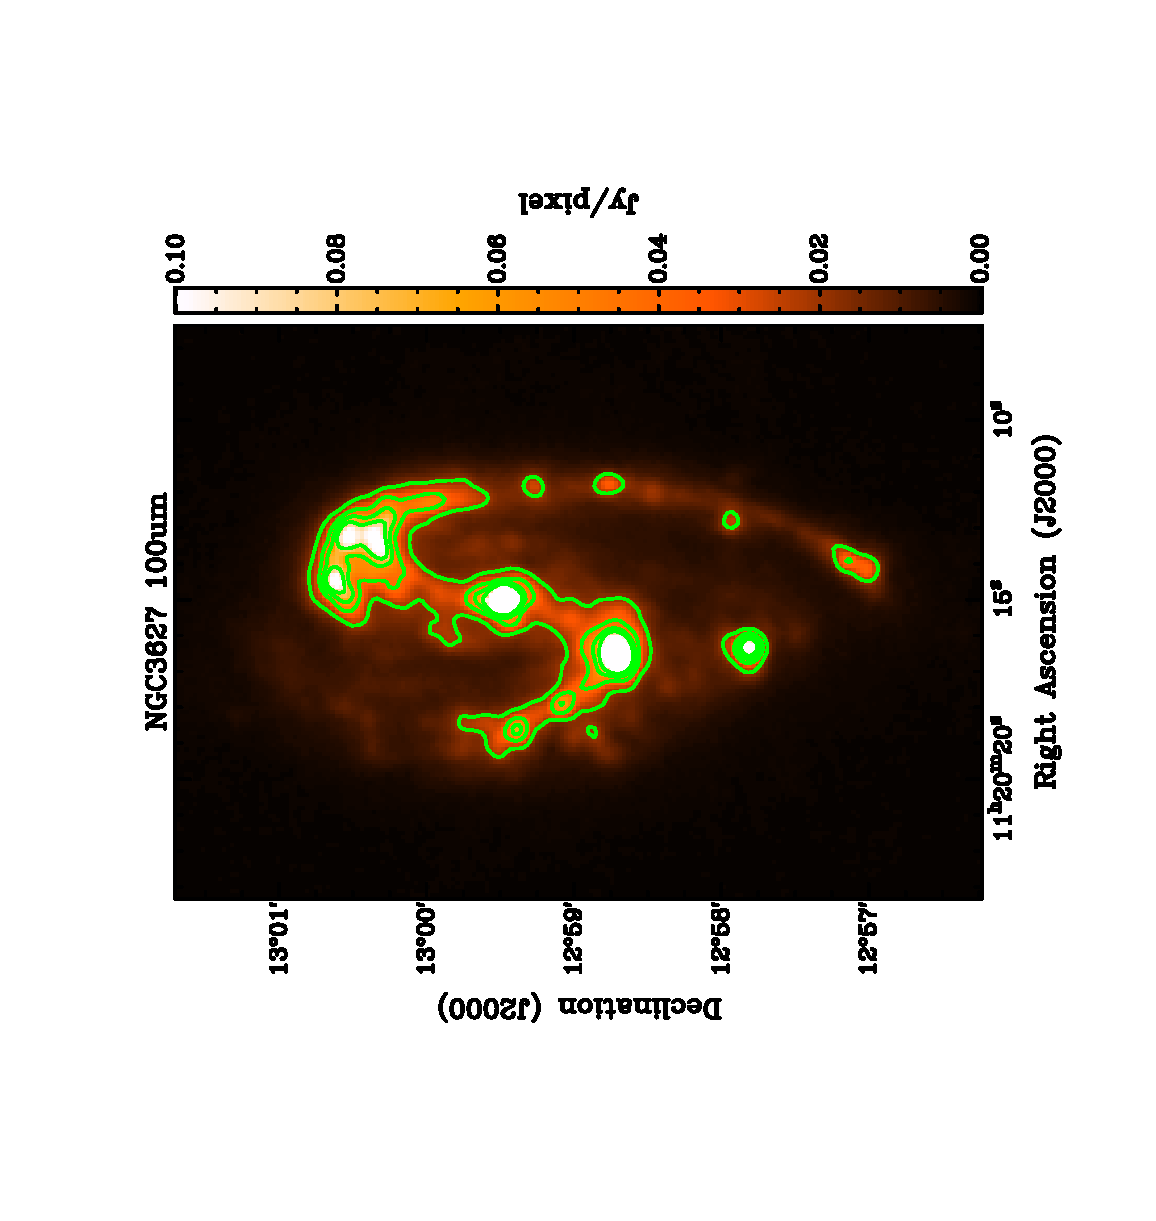
\includegraphics[width=1.\linewidth, angle=270]{obs_imgs/100_orig.eps}
    \caption{Herschel 100$\mu$m image of NGC3627 with 1.7$\arcsec$ by 1.7$\arcsec$ pixels.}
  \end{subfigure}%
  \quad
  \begin{subfigure}[t]{.48\textwidth}
    \centering
    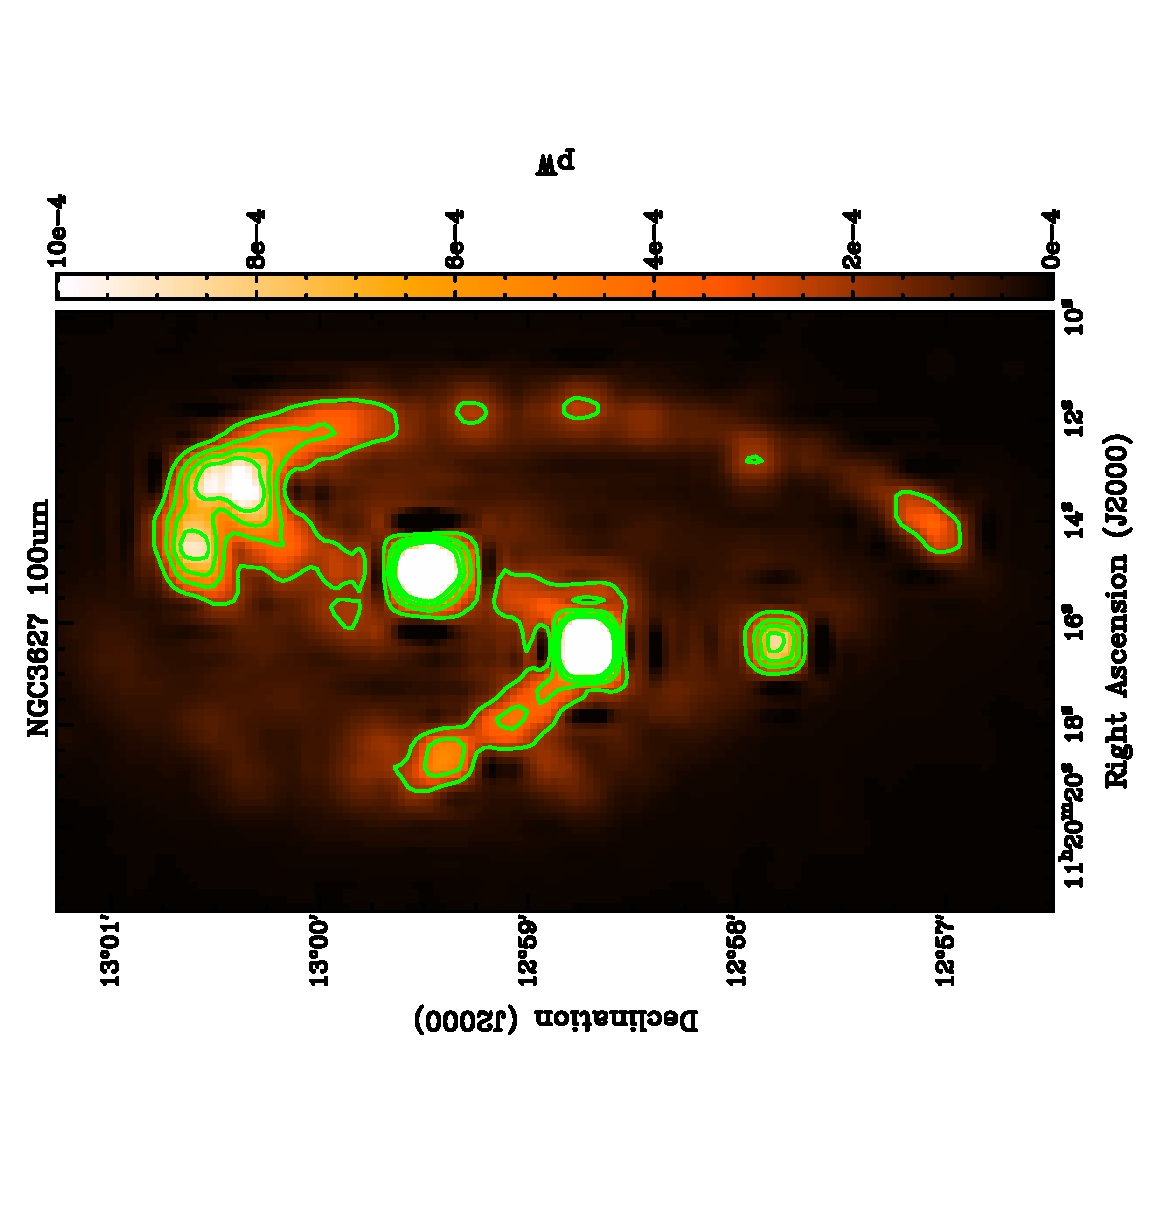
\includegraphics[width=1.\linewidth, angle=270]{obs_imgs/100_align.eps}
    \caption{Herschel 100$\mu$m image converted to pW and rescaled to a 2$\arcsec$ by 2$\arcsec$ pixel grid.}
  \end{subfigure}%

  \begin{subfigure}[t]{.45\textwidth}
    \centering
    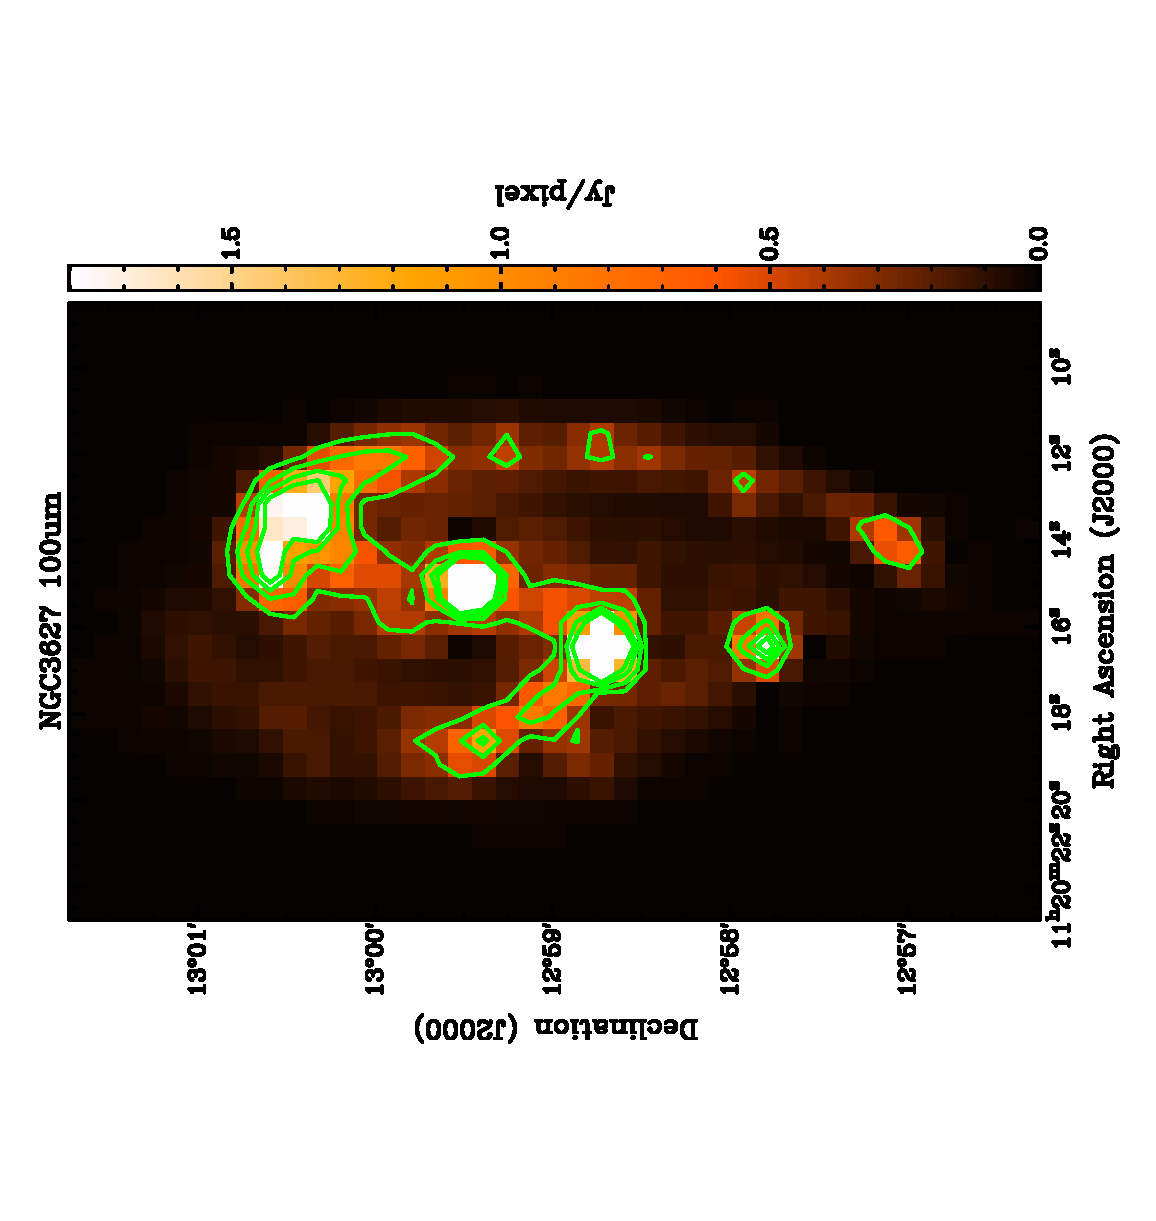
\includegraphics[width=1.\textwidth,angle=270]{obs_imgs/100_rem.eps}
    \caption{100$\mu$m map of NGC3627 after large scale structure has been removed and rescaled to an 8$\arcsec$ by 8$\arcsec$ grid.}
  \end{subfigure}%
  \quad
  \begin{subfigure}[t]{0.45\textwidth}
    \centering
    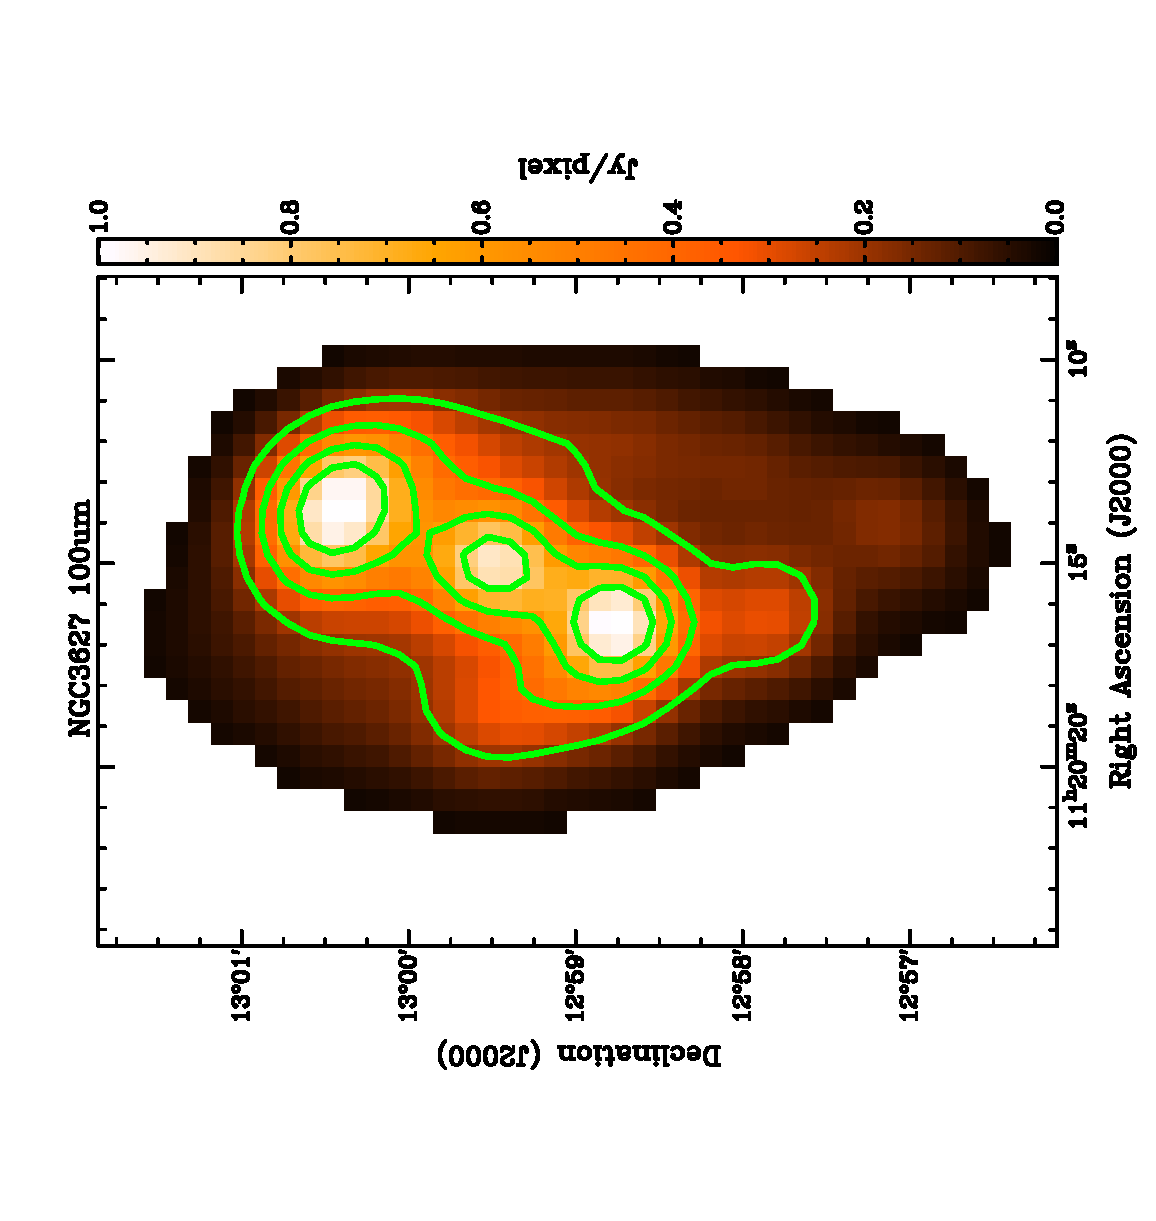
\includegraphics[width=1.\textwidth,angle=270]{obs_imgs/100_sed_use.eps}
    \caption[100$\mu$m Filtering Steps]{100$\mu$m map with extended structure removed and convolved to final resolution of 36.0$\arcsec$ with a 5$\sigma$ cut applied.}
  \end{subfigure}
  \caption[100$\mu$m Filtering Steps]{The 100$\mu$m image from the beginning of processing to the end of processing.  All of the contours shown are 20\%, 40\%, 60\%, and 80\%.}
  \label{fig_100_transform}
\end{figure}
  

The rest of the ancillary data are used in calculating a dust to gas ratio, and follow nearly the same process as the SED data filtering.  The major difference is the CO J=1-0, CO J=2-1 and HI maps need to remain in their original units of K km/s and M$_\odot$/pc$^2$.  This requirement simplified the process by only requiring a scaling factor of 0.001 to be applied to the original maps.  After the image is scaled, it is filtered using the fakesource option in MAKEMAP with the 850$\mu$m observation as the base image.  The atomic and molecular gas maps were then isolated in the same fashion as the KINGFISH and NGLS by subtracting the 850$\mu$m map.  Then they were rescaled back to their original values, fit to an 8$\arcsec$ by 8$\arcsec$ grid and finally convolved to a 36.0$\arcsec$ resolution.  The process is illustrated in Figure \ref{fig_HI_transform}.  The amount of emission lost is shown in tables \ref{tab_obs_n45}, \ref{tab_obs_heracles}, and \ref{tab_obs_things}.

\begin{figure}
  \centering
  \begin{subfigure}[t]{.48\textwidth}
    \centering
    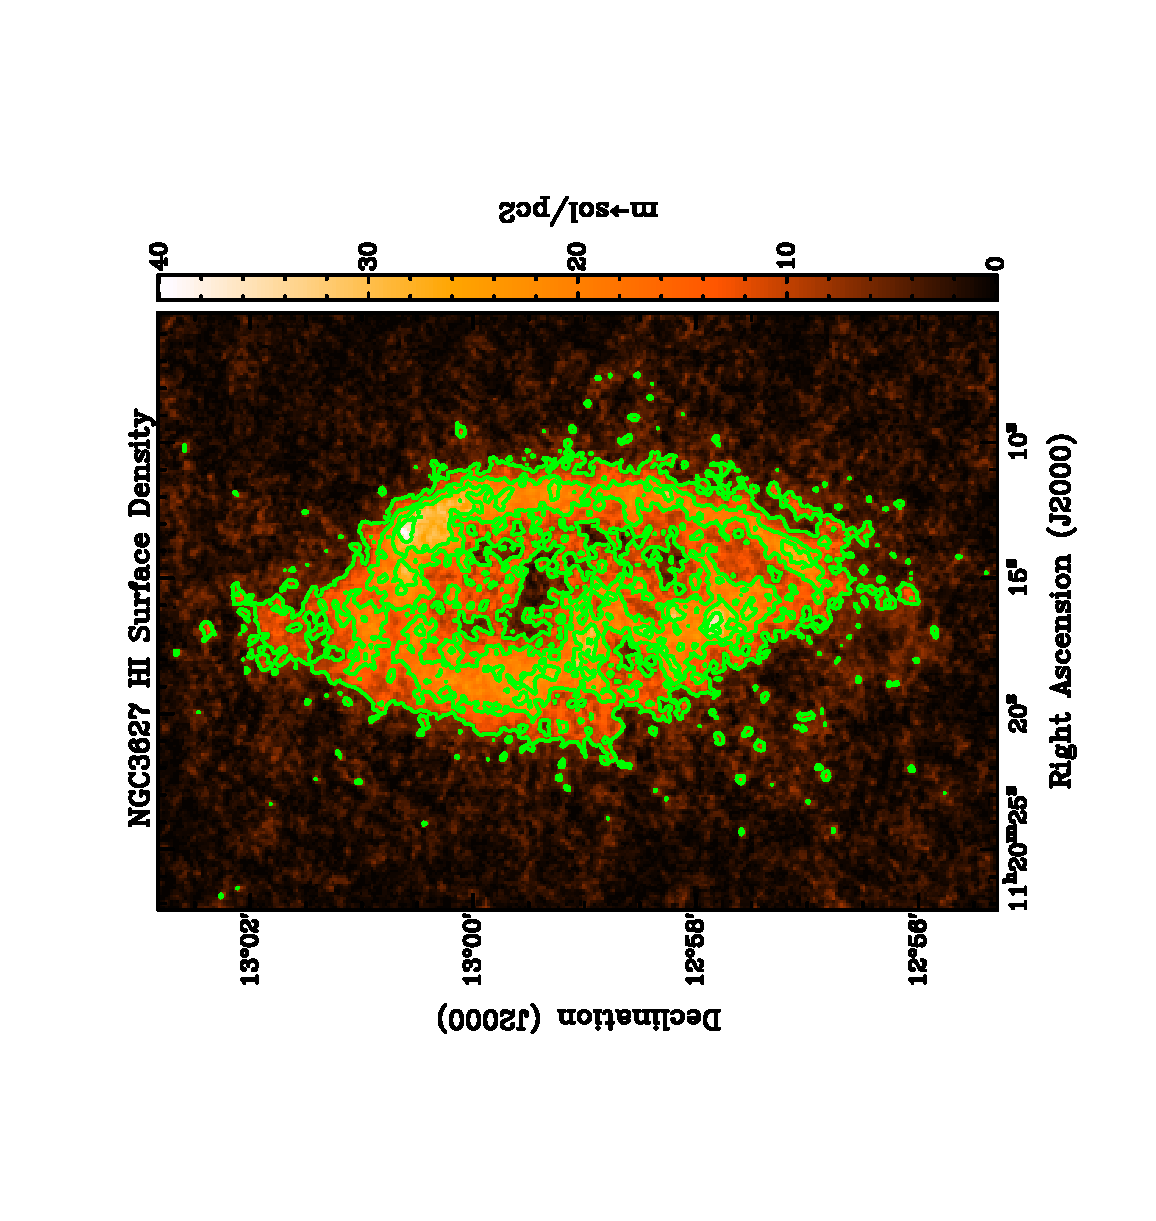
\includegraphics[width=1.\linewidth, angle=270]{obs_imgs/HI_orig.eps}
    \caption{HI surface density map of NGC3627 with 1.5$\arcsec$ by 1.5$\arcsec$ pixels.}
  \end{subfigure}%
  \quad
  \begin{subfigure}[t]{.48\textwidth}
    \centering
    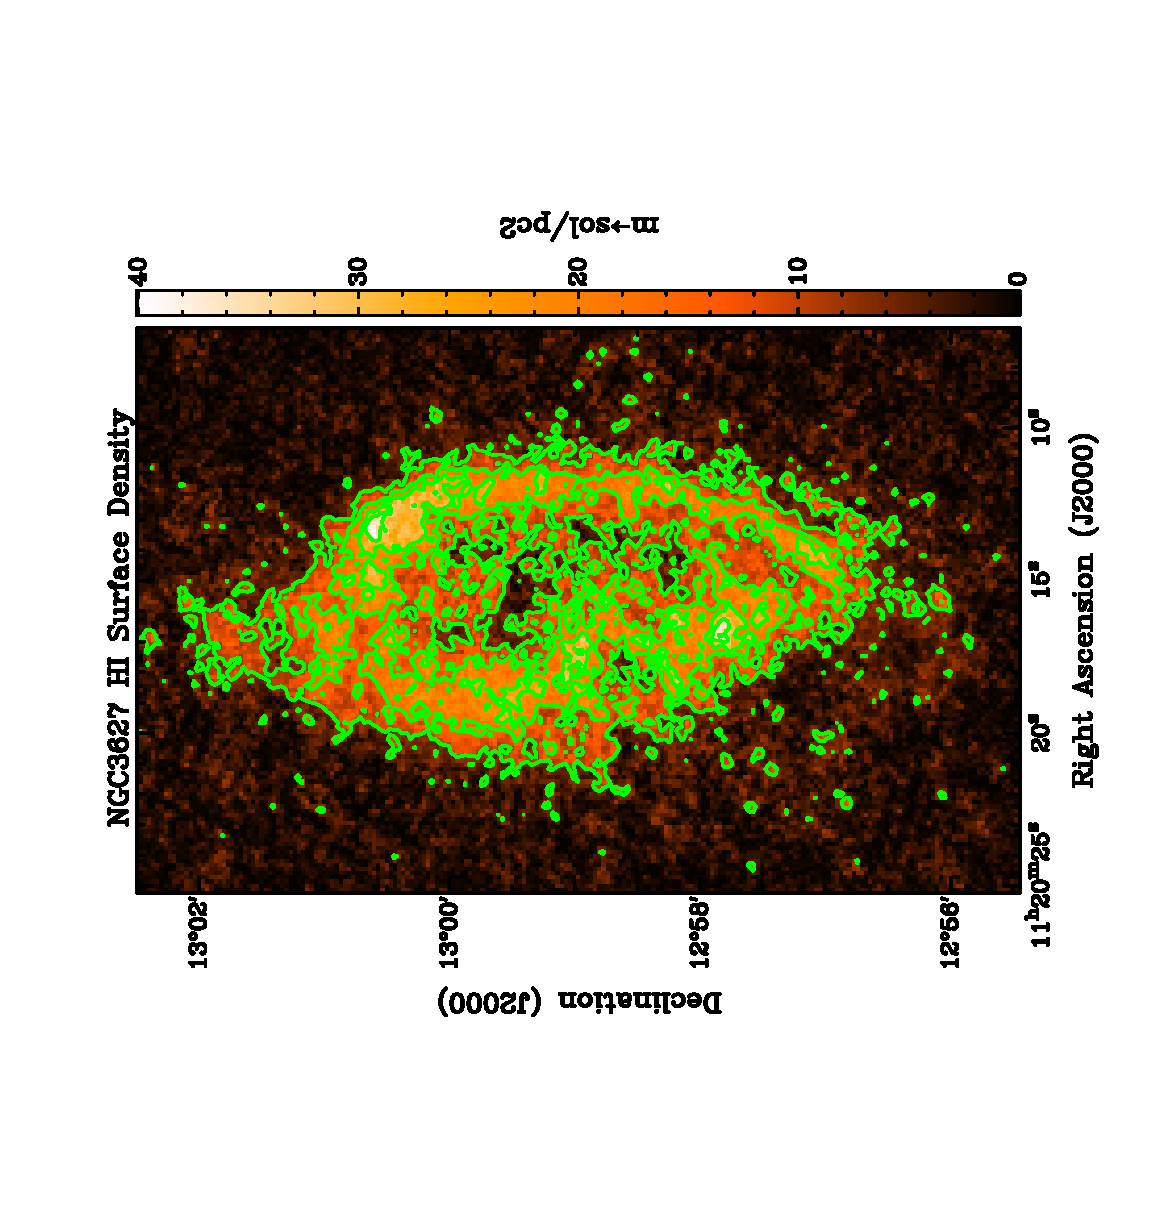
\includegraphics[width=1.\linewidth, angle=270]{obs_imgs/HI_align.eps}
    \caption{HI surface density map rescaled to a 2$\arcsec$ by 2$\arcsec$ pixel grid.}
  \end{subfigure}%

  \begin{subfigure}[t]{.45\textwidth}
    \centering
    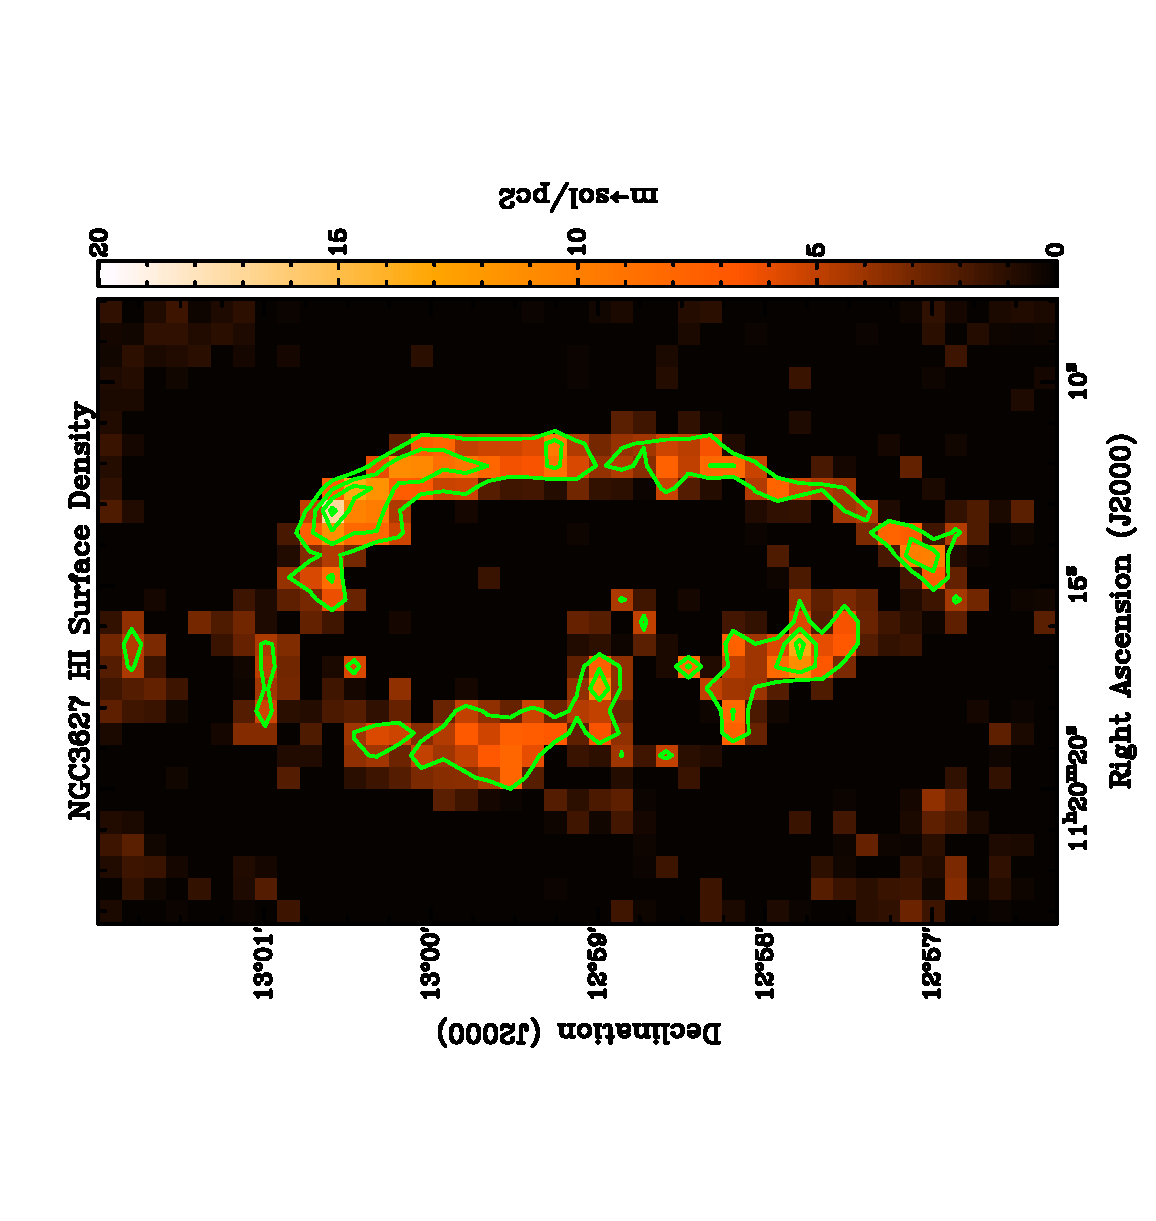
\includegraphics[width=1.\textwidth,angle=270]{obs_imgs/HI_rem.eps}
    \caption{HI surface density map of NGC3627 after large scale structure has been removed and rescaled to an 8$\arcsec$ by 8$\arcsec$ grid.}
  \end{subfigure}%
  \quad
  \begin{subfigure}[t]{0.45\textwidth}
    \centering
    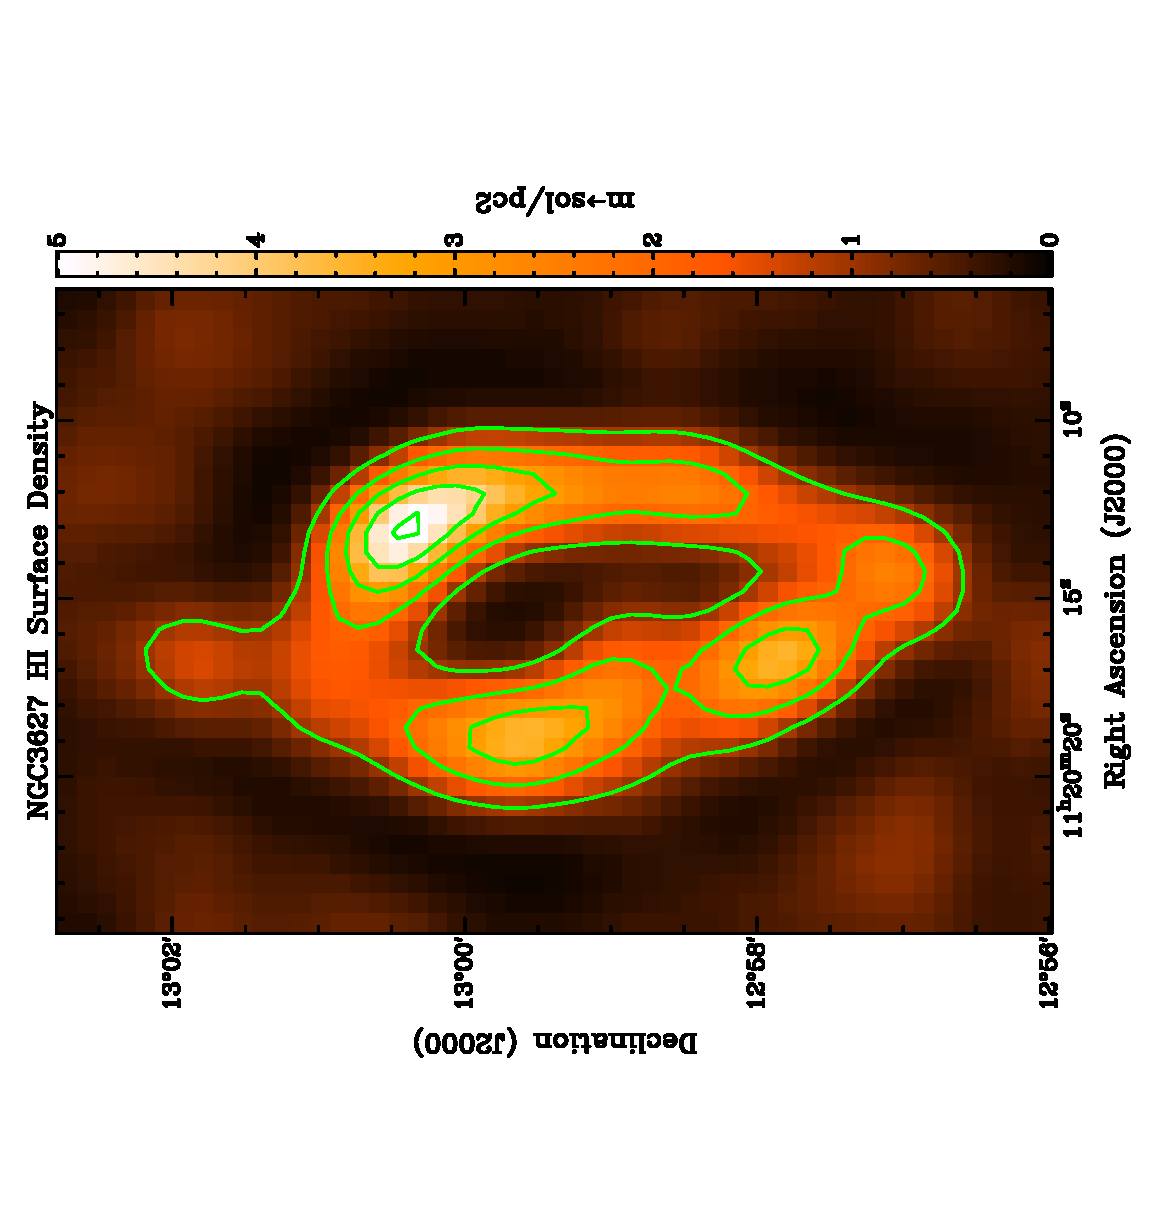
\includegraphics[width=1.\textwidth,angle=270]{obs_imgs/HI_use.eps}
    \caption[100$\mu$m Filtering Steps]{HI surface density map with extended structure removed and convolved to final resolution of 36.0$\arcsec$.}
  \end{subfigure}
  \caption[HI surface density filtering Steps]{The HI surface density maps from the beginning of processing to the end of processing.  The contours in the top row are 30\%, 60\% and 90\%, and the contours in the bottom row are 20\%, 40\%, 60\%, and 80\%.}
  \label{fig_HI_transform}
\end{figure}
 

\chapter{Spectral Energy Distribution Analysis}

\section{SED Fitting Method}

In order to determine a dust mass, we use the IDL package MPFIT \citep{markwardt2009} to fit equation \ref{eq:mod_sed} for the temperature, T, mass, M, and the emissivity index, $\beta$.  The routine MPFIT utilizes the Levenberg-Marquardt algorithm.  This algorithm uses a combination of two minimization techniques (the steepest descent method and the Newton-Raphson Method) to determine the parameter combination that corresponds to a minimum in the $\chi^2$ space while maximizing the efficiency of the step sizes in each iteration \citep{burden2001}.  The algorithm begins by implementing the steepest descent method.  This working of this technique is to follow the direction opposite of the largest gradient in order to traverse the $\chi^2$ space to locate a minimum.  As the set of solutions approaches a minimum, it will switch to the Newton-Raphson method to locate the best set of parameters by finding where the derivative at that point is closest to zero \citep{gavin2013}.  

\begin{equation}\label{eq:mod_sed}
  S_\nu\left(T\right) = \frac{M\:\kappa_{\nu,0}}{D^2}\left(\frac{\nu}{\nu_0}\right)^{\beta+3} B_\nu\left(T\right)
\end{equation}

In order for MPFIT to provide the most accurate fit, we establish a reasonable error for each of our data points, and determine a realistic set of starting points for the fitting.  The variance for our SCUBA-2 data is determined by equation \ref{eq:sc2noi} such that $\sigma_{obs}$ is the noise determined by MAKEMAP, $\sigma_{rms,sky}$ is the RMS of the sky, and $\sigma_{calib}$ is the calibration uncertainties where the scaling factor is shown in table \ref{tab:calib_fac}.

\begin{equation}\label{eq:sc2noi}
  \sigma^2 = \sigma_{obs}^2 + \sigma_{rms,sky}^2 + \sigma_{calib}^2
\end{equation}

\begin{deluxetable}{cc}
%  \tabletypesize{\footnotesize}
  \tablecolumns{2}
  \tablewidth{0pt}
  \tablecaption{Calibration Factors for SCUBA-2 and KINGFISH Observations\label{tab:calib_fac}}
  \tablehead{\colhead{Observation} & \colhead{Scaling Factor}}
    \startdata
      100$\mu$m & 0.03 \\
      160$\mu$m & 0.05 \\
      250$\mu$m & 0.07 \\
      350$\mu$m & 0.07 \\
      450$\mu$m & 0.12 \\
      500$\mu$m & 0.07 \\
      850$\mu$m & 0.08 \\
    \enddata
\end{deluxetable} 

The variance for the KINGFISH data are determined in a similar fashion and are shown in equation \ref{eq:kinnoi}, however the observation error is excluded since the reported variance in the filtered images are reflective of the fake source image used and not of the KINGFISH data set.

\begin{equation}\label{eq:kinnoi}
  \sigma^2 = \sigma_{rms,sky}^2 + \sigma_{calib}^2
\end{equation}

The nature of the Levinberg-Marquardt method leaves the solution vulnerable to converge at a local minimum rather than converging at the global minimum.  This is remedied by selecting reasonable initial conditions.  The initial conditions we used were  a modified blackbody with a temperature of 20K, a dust emissivity index of 2, and a mass determined by equation \ref{eq:mass} using the flux from the 250$\mu$m emission and our initial temperature and dust emissivity values.  

\begin{equation}\label{eq:mass}
  \begin{split}
    M & = \frac{D^2 \: I_{250}}{\kappa_{\nu,0} \:  B_{250}\left(T\right)} \left(\frac{\nu}{\nu_0} \right)^{-\left(\beta+3\right)} \\
      & = 2.24 \times 10^5 \: I_{250} \; \left[M_\odot\right]
  \end{split}
\end{equation}

\section{Fitting the Spectral Energy Distribution}

The fitting procedure was carried out in two different ways on a modified blackbody equation, equation \ref{eq:mod_sed}.  One of the two methods is fitting an SED to each individual pixel in order to generate a set of parameter maps, and the second is by totaling the flux of each of the selected regions shown in figure \ref{fig:regions} to maximize the signal to noise ratio in order to generate a more precise set of parameters.  For both of the fitting methods the mass, $M$, and temperature, $T$, are set as free parameters, but the treatment of the emissivity index, $\beta$, required special treatment for each of the methods.  The distance, D, has been set to 9.4 Mpc \citep{walter2008}, and the reference opacity, $\kappa_{\nu,0}$, was tested using 0.2665 m$^2$ kg$-1$ \citep{li2001} and 1.0 m$^-2$ kg$^-1$ \citep{planckxxv2011}.

\begin{figure}
  \centering
  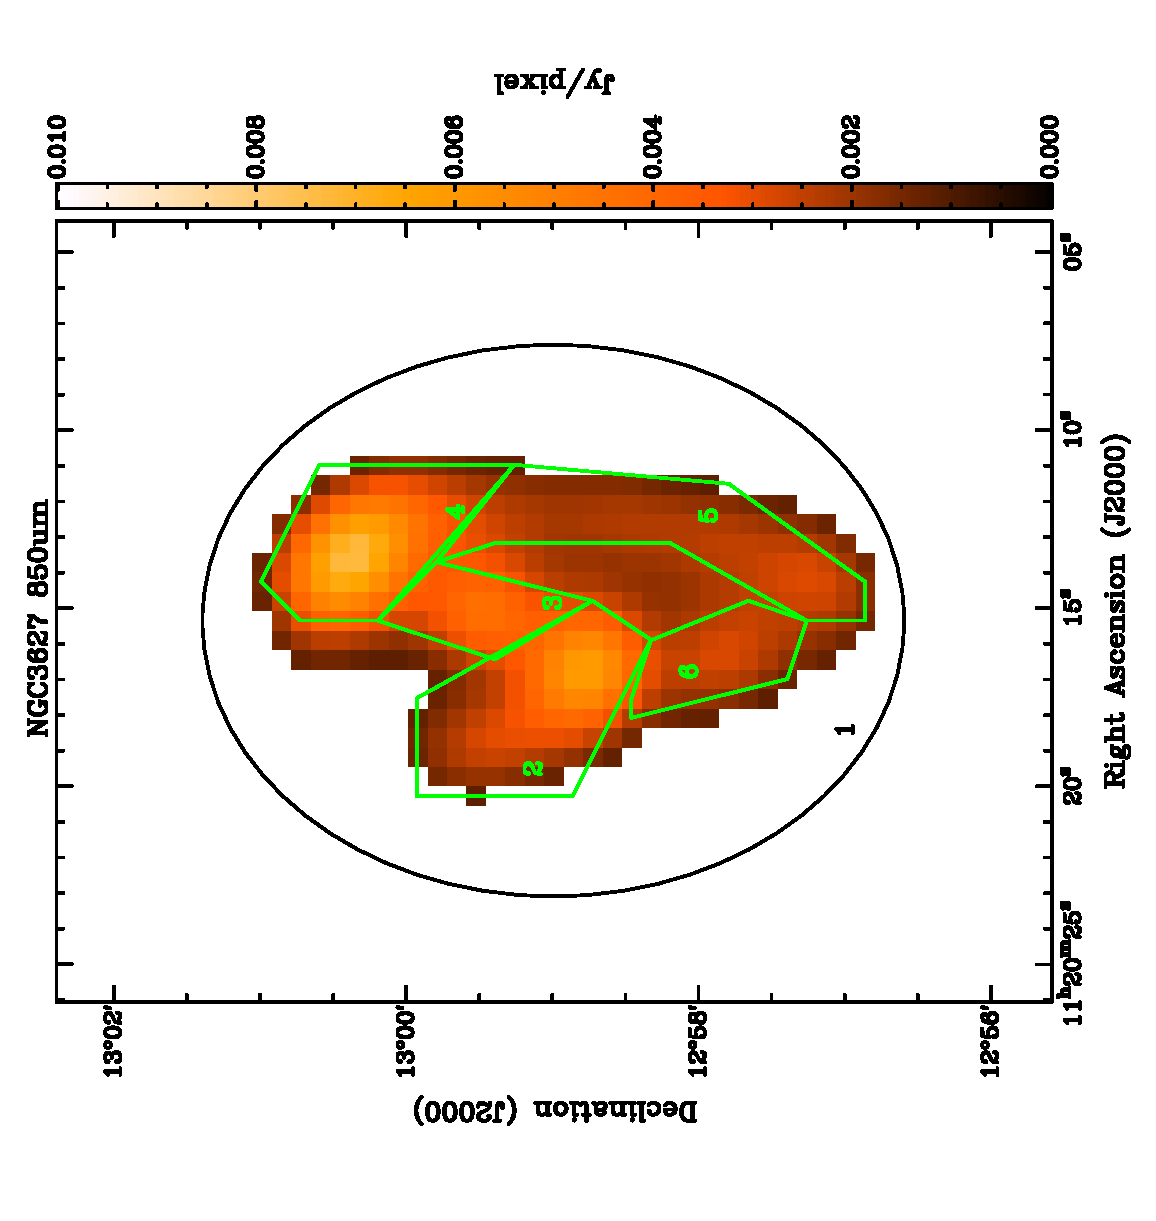
\includegraphics[width=1.\textwidth,angle=270]{sed_imgs/regions.eps}
  \caption[NGC3627 Regions]{850$\mu$m emission convolved to the 500$\mu$m beam size overlaid with the selected regions of NGC3627 labeled 1 through 6 such that region 1 includes the entire galaxy.}
  \label{fig:regions}
\end{figure}

\subsection{Pixel SED Fits}

In order to generate a parameter map of NGC3627, each individual pixel has it's own SED determined from the available wavelengths described in the observations chapter.  Initially, we exclude the 500$\mu$m emission, and in later fits, we substitute the 450$\mu$m emission with 500$\mu$m emission.  The treatment of the dust emissivity index is performed by fixing it at $\beta=1.8$ for the Planck opacity model such that the opacity is $\kappa_{300\mu m,0}=1.0$ m$^2$ kg$^{-1}$ \citep{planckxxv2011} and $\beta=2.0$ for the Li and Draine opacity model where the opacity is $\kappa_{300\mu m,0}=0.2665$ m$^2$ kg$^{-1}$ \citep{li2001}.  A third fit is performed where the emissivity index is allowed to vary as a free parameter.  While the emissivity index is allowed to vary, the opacity being used is the Planck model in order to generate a minimum mass estimate of the two opacity values.  Using either an opacity of 1.0 m$^2$ kg$^{-1}$ or 0.2665 m$^2$ kg$^{-1}$ will not effect the shape of the SED, only the its normalizing value.  In the case of our fits, it is the mass that acts as the normalizing constant, so increasing or decreasing the opacity will yield the opposite effect in the mass.  The inverse proportionality can be seen in equation \ref{eq:mass}.  The resulting parameter maps of the fits are shown in figure \ref{fig:param_fits}. The numerical values from fitting each model are shown in tables \ref{tab:beta_1}, \ref{tab:beta_2}, and \ref{tab:beta_f} where each region corresponds to the regions labeled in figure \ref{fig:regions}.

\begin{figure}
  \centering
  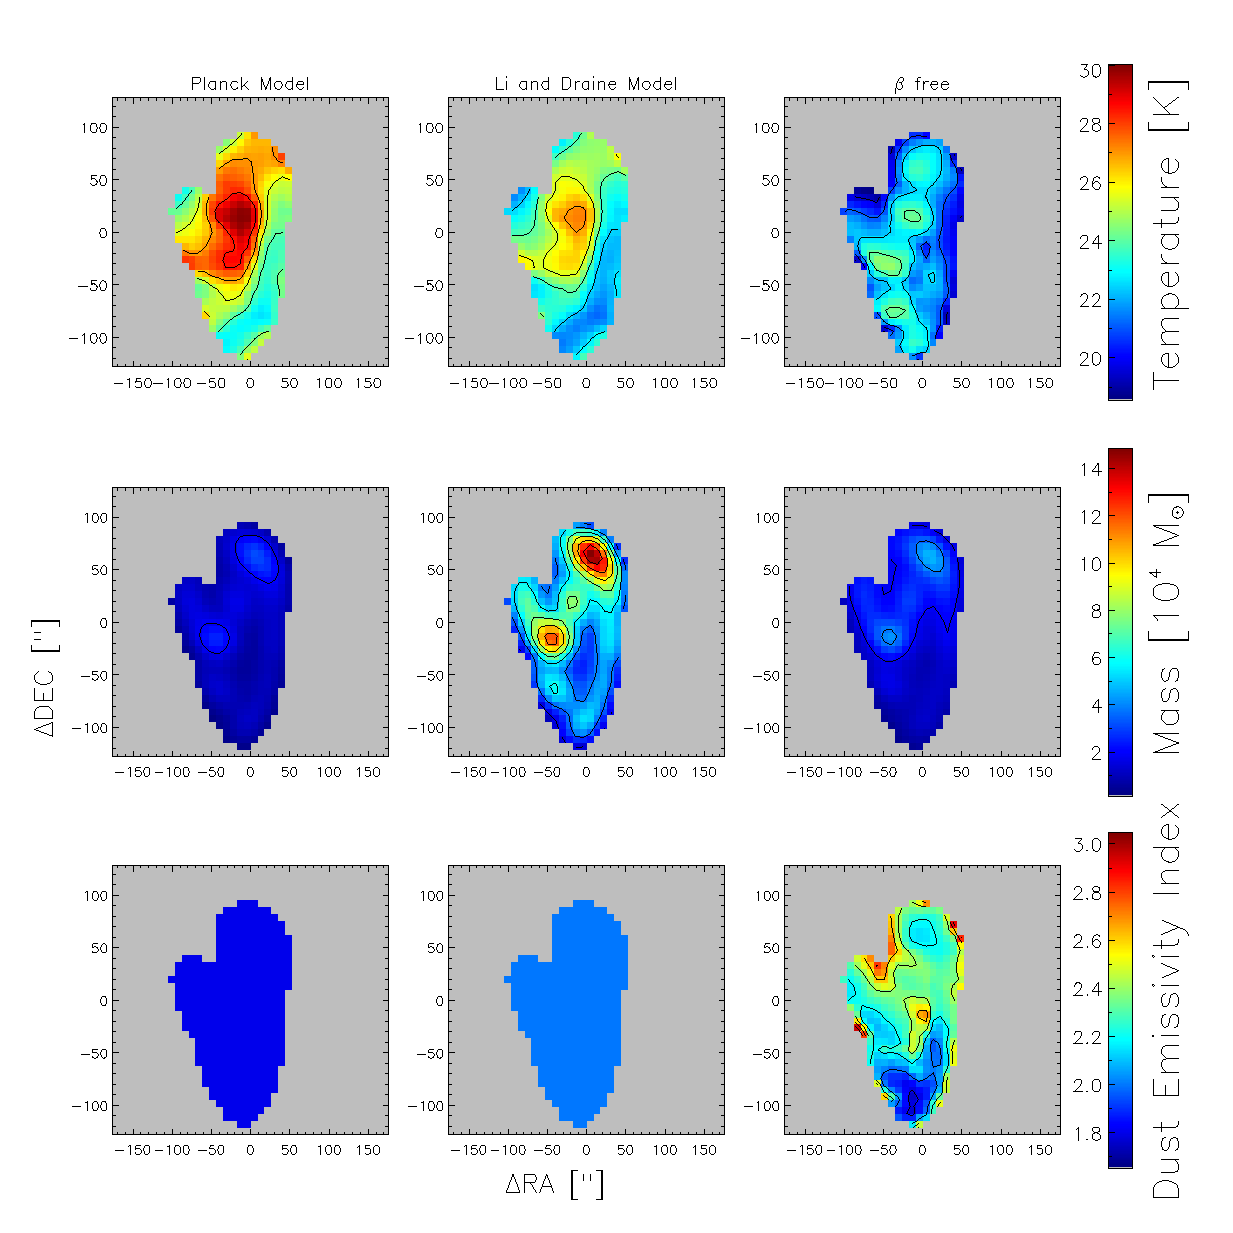
\includegraphics[width=1.\textwidth]{sed_imgs/parameter_full.eps}
  \caption[SED Parameter Maps]{Returned value for the SED fits with the Planck model in the left column, the Li and Draine model  in the middle column, and $\beta$ as a free variable in the right column.  The top row shows the temperature with contours from 1.5K to 28.5K in 1.5K increments.  The second row show the returned masses with contours from 1.9M$_\odot$ to 13.3M$_\odot$ in 1.9M$_\odot$ increments.  The Li and Draine mass fits have been divided by three to better show the features.  Th bottom row shows the returned dust emissivity index values with contours from 1.8 to 2.8 with 0.2 increments.}
  \label{fig:param_fits}
\end{figure}

\begin{deluxetable}{ccccc}
  \tablecolumns{5}
  \tablewidth{0pt}
  \tablecaption{Best Fit Parameters for Planck Model\label{tab:beta_1}}
  \tablehead{\colhead{Region} & \colhead{Average $\beta$} & \colhead{ Total Mass} & \colhead{Surface Density} & \colhead{Average Temperature} \\ & &  $\left[10^5M_\odot\right]$ & $\left[M_\odot pc^{-2}\right]$ &[K]}
  \startdata
    1 & 1.8 & 47  $\pm$ 22  & 0.09 $\pm$ 0.04 & 26   $\pm$ 2   \\
    2 & 1.8 & 12  $\pm$ 4   & 0.11 $\pm$ 0.04 & 27   $\pm$ 2   \\
    3 & 1.8 & 5   $\pm$ 1   & 0.10 $\pm$ 0.02 & 28.8 $\pm$ 0.6 \\
    4 & 1.8 & 14  $\pm$ 5   & 0.14 $\pm$ 0.05 & 26   $\pm$ 1   \\
    5 & 1.8 & 9   $\pm$ 2   & 0.07 $\pm$ 0.02 & 24   $\pm$ 1   \\
    6 & 1.8 & 3.8 $\pm$ 0.9 & 0.07 $\pm$ 0.02 & 25   $\pm$ 1   \\
  \enddata
\end{deluxetable}

\begin{deluxetable}{ccccc}
  \tablecolumns{5}
  \tablewidth{0pt}
  \tablecaption{Best Fit Parameters for Li and Draine Model\label{tab:beta_2}}
  \tablehead{\colhead{Region} & \colhead{Average $\beta$} & \colhead{ Total Mass} & \colhead{Surface Density} & \colhead{Average Temperature} \\ & &  $\left[10^5M_\odot\right]$ & $\left[M_\odot pc^{-2}\right]$ &[K]}
  \startdata
    1 & 2.0 & 219 $\pm$ 103 & 0.4  $\pm$ 0.2  & 24   $\pm$ 2   \\
    2 & 2.0 & 54  $\pm$ 19  & 0.5  $\pm$ 0.2  & 25   $\pm$ 1   \\
    3 & 2.0 & 26  $\pm$ 5   & 0.48 $\pm$ 0.09 & 26.4 $\pm$ 0.5 \\
    4 & 2.0 & 67  $\pm$ 23  & 0.7  $\pm$ 0.2  & 24.4 $\pm$ 0.8 \\
    5 & 2.0 & 40  $\pm$ 9   & 0.33 $\pm$ 0.07 & 22.4 $\pm$ 0.9 \\
    6 & 2.0 & 17  $\pm$ 4   & 0.32 $\pm$ 0.08 & 23.5 $\pm$ 0.9 \\
  \enddata
\end{deluxetable}

\begin{deluxetable}{ccccc}
  \tablecolumns{5}
  \tablewidth{0pt}
  \tablecaption{Best Fit Parameters for $\beta$ As A Free Parameter\label{tab:beta_f}}
  \tablehead{\colhead{Region} & \colhead{Average $\beta$} & \colhead{ Total Mass} & \colhead{Surface Density} & \colhead{Average Temperature} \\ & &  $\left[M_\odot\right]$ & $\left[10^5M_\odot pc^{-2}\right]$ &[K]}
  \startdata
    1 & 2.2  $\pm$ 0.2  & 73 $\pm$ 35 & 0.14 $\pm$ 0.06 & 22   $\pm$ 1   \\
    2 & 2.3  $\pm$ 0.2  & 19 $\pm$ 6  & 0.18 $\pm$ 0.05 & 22   $\pm$ 2   \\
    3 & 2.34 $\pm$ 0.09 & 9  $\pm$ 1  & 0.18 $\pm$ 0.02 & 23.0 $\pm$ 0.9 \\
    4 & 2.2  $\pm$ 0.1  & 22 $\pm$ 6  & 0.21 $\pm$ 0.05 & 22   $\pm$ 1   \\
    5 & 2.1  $\pm$ 0.2  & 12 $\pm$ 4  & 0.10 $\pm$ 0.03 & 22   $\pm$ 1   \\
    6 & 2.1  $\pm$ 0.1  & 5  $\pm$ 1  & 0.09 $\pm$ 0.02 & 23.0 $\pm$ 0.9 \\
  \enddata
\end{deluxetable}

The wellness of each fit is shown figures \ref{fig:w1_4}, \ref{fig:w2_4}, and \ref{fig:wf_4} for the Plank model, Li and Draine model, and beta as a free parameter respectively.  The quality of the fit is determined by how well the expected flux from the SED fitting matches the observed flux.  If the fits are able to recreate the observed emission, then all of the points will lie on the line $y=x$ shown in the plots as a black line.  If the SED is underestimating the flux, the points will appear below the 1 to 1 line, and an over estimation from the SED will result in points above the line.  

\begin{figure}
  \centering
  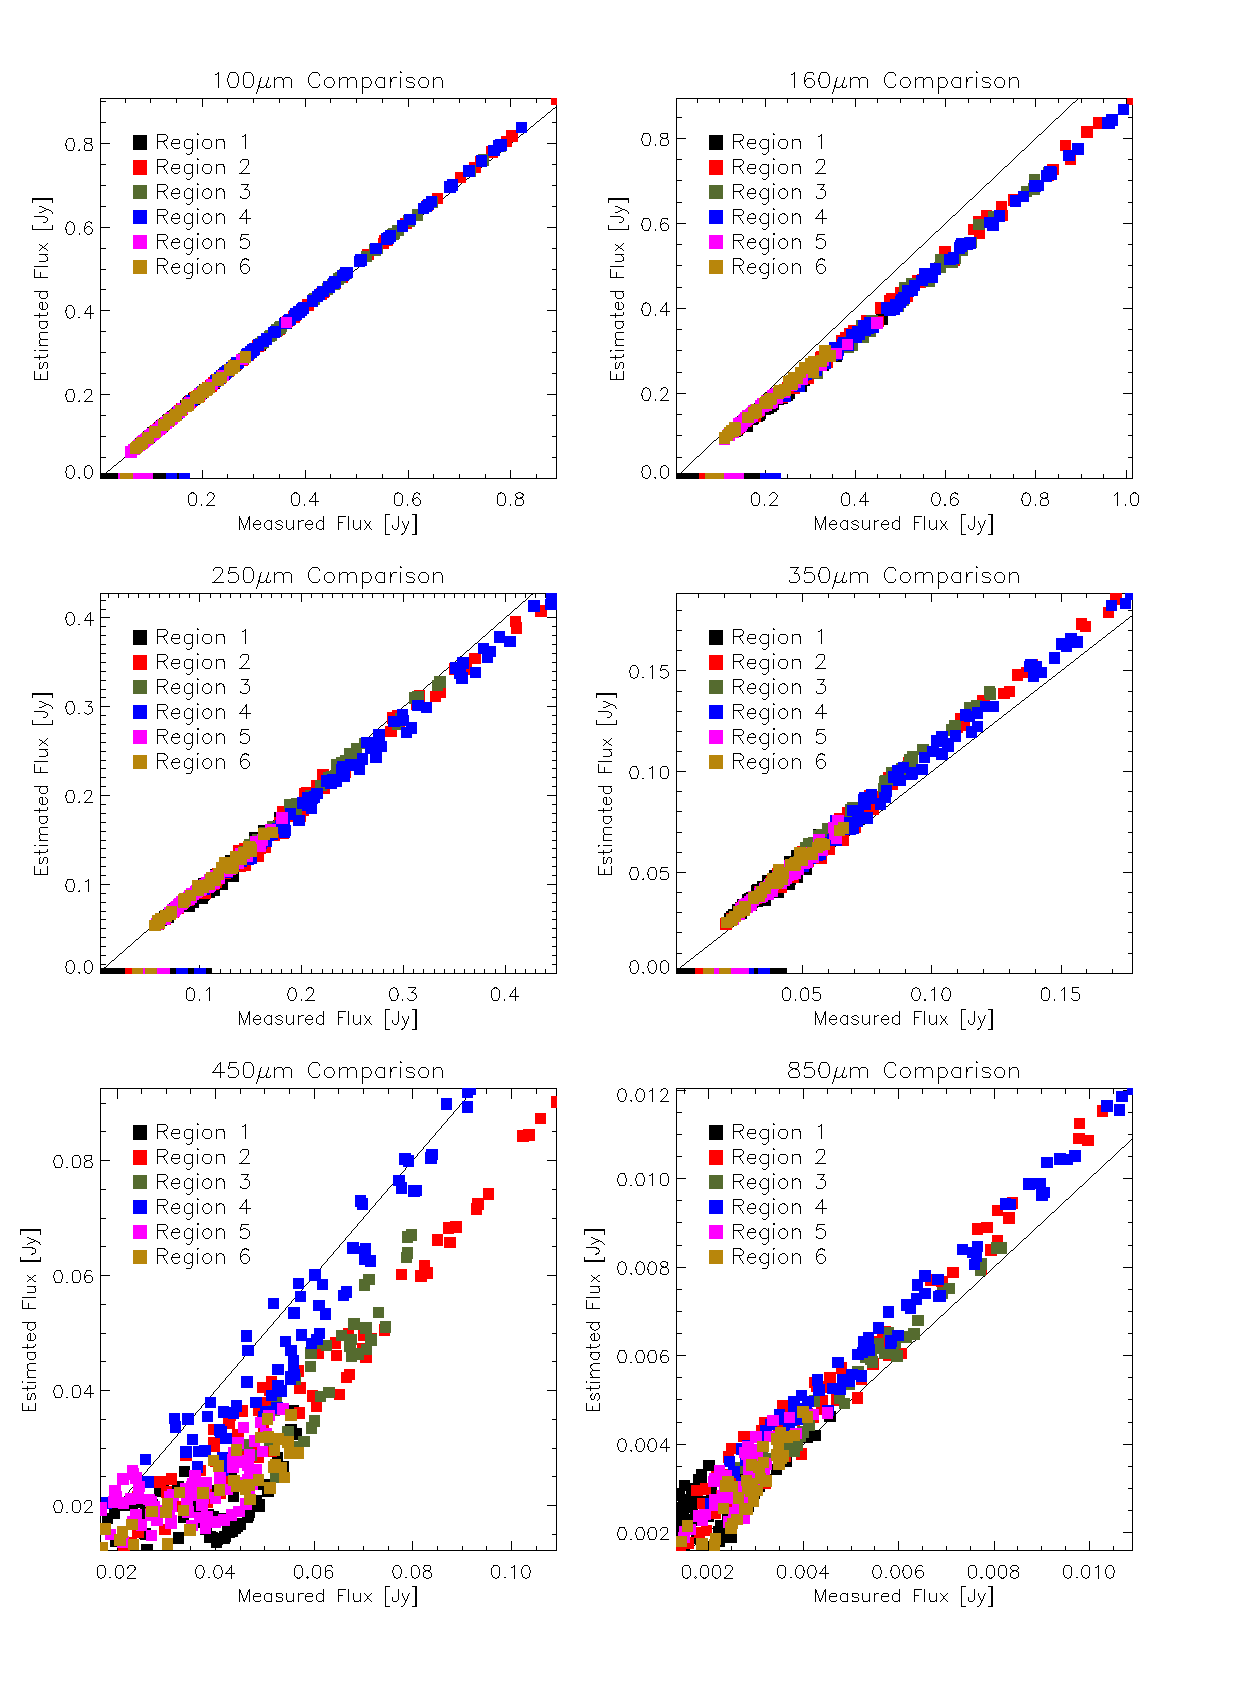
\includegraphics[width=1.\textwidth]{sed_imgs/flux_compare_1_4.eps}
  \caption[Planck Model SED Fit Quality Using 450$\mu$m Data]{Quality of the SED fits to the Planck model using the 450$\mu$m emission.  The regions shown are the regions in figure \ref{fig:regions}.}
  \label{fig:w1_4}
\end{figure}

\begin{figure}
  \centering
  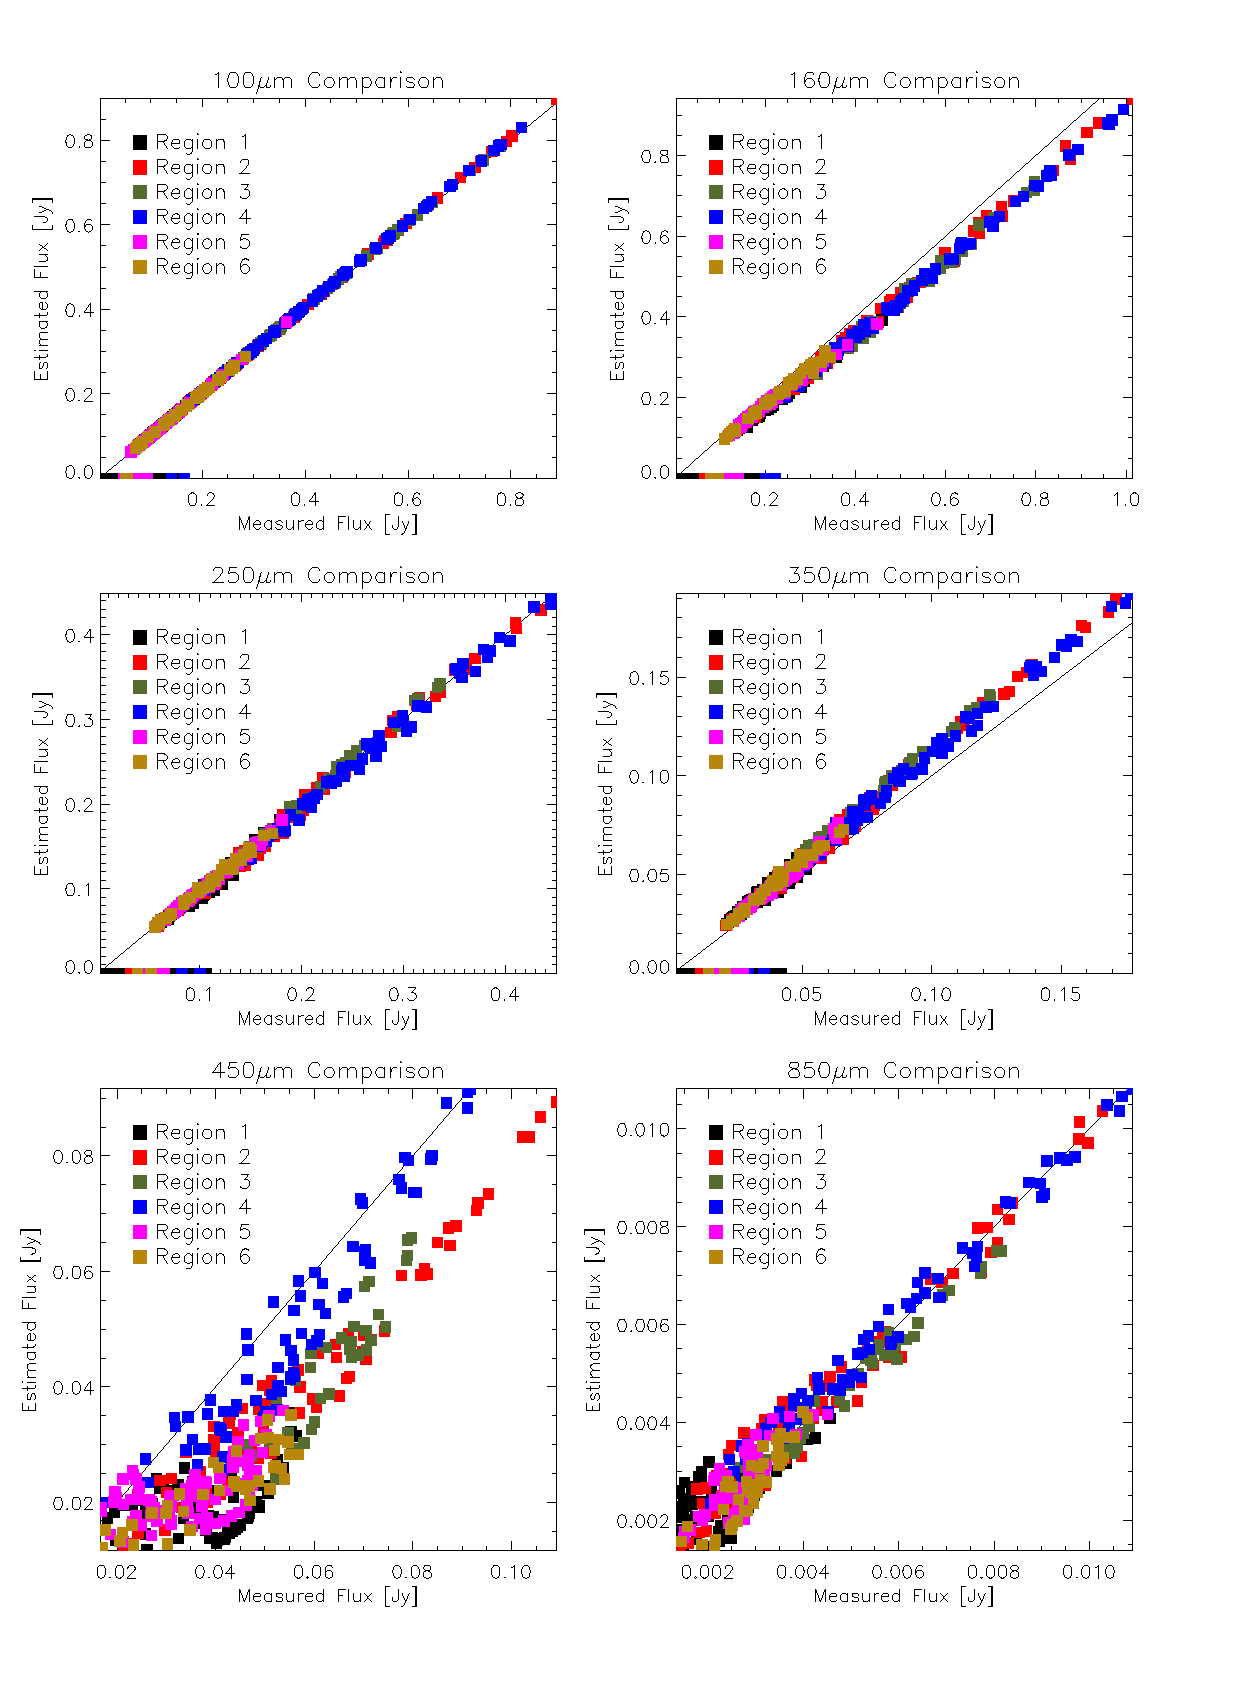
\includegraphics[width=1.\textwidth]{sed_imgs/flux_compare_2_4.eps}
  \caption[Li and Draine Model SED Fit Quality Using 450$\mu$m Data]{Quality of the SED fits to the Li and Draine model using the 450$\mu$m emission.  The regions shown are the regions in figure \ref{fig:regions}.}
  \label{fig:w2_4}
\end{figure}

\begin{figure}
  \centering
  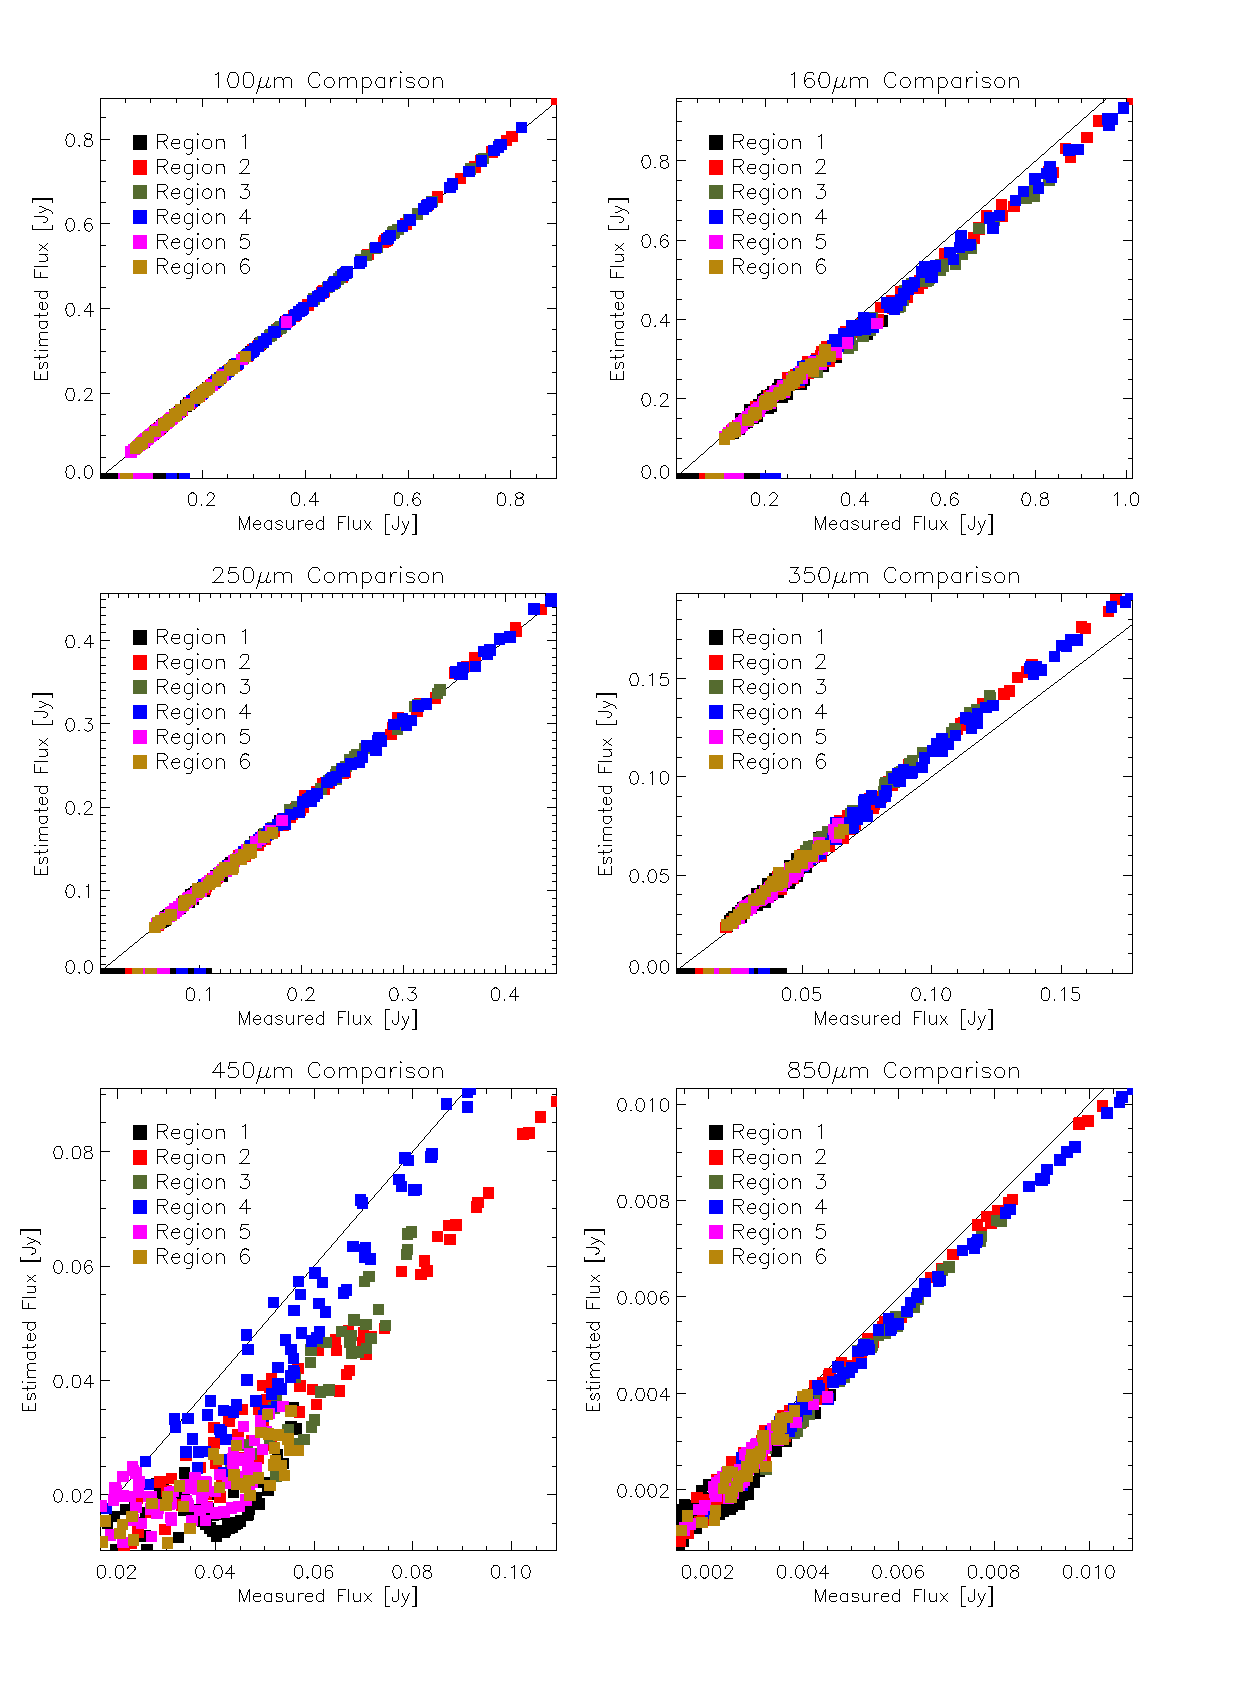
\includegraphics[width=1.\textwidth]{sed_imgs/flux_compare_free_4.eps}
  \caption[Emissivity as a Free Parameter SED Fit Quality Using 450$\mu$m Data]{Quality of the SED fits with the dust emissivity index as a free parameter using the 450$\mu$m emission.  The regions shown are the regions in figure \ref{fig:regions}.}
  \label{fig:wf_4}
\end{figure}

Using these plots, it is clear that the SED is over estimating the 450$\mu$m flux despite the care taken while accounting for the odd beam shape of the 450$\mu$m data.  This overestimation was not a result of a poor fit, but rather a calibration error in the 450$\mu$m observations.  The intrinsic error to the SCUBA-2 450$\mu$m data was determined by extrapolating an expected value from the 350$\mu$m and 500$\mu$m KINGFISH data assuming the decrease in intensity was linear.  In order to avoid any errors in our final parameter maps, we substitute the 450$\mu$m emission with KINGFISH 500$\mu$m emission.  The quality of fit maps using the 500$\mu$m emission are shown in figures \ref{fig:w1_5}, \ref{fig:w2_5}, and \ref{fig:wf_5} for the Planck model, Li and Draine model and the emissivity as a free parameter respectively.  To assign a numerical quantity to the vertical distance was calculated for each point to the 1 to 1 line and then summed.  The summed distances are shown in table \ref{tab:lsq} and suggest the best fit comes from allowing the emissivity index to vary.

\begin{figure}
  \centering
  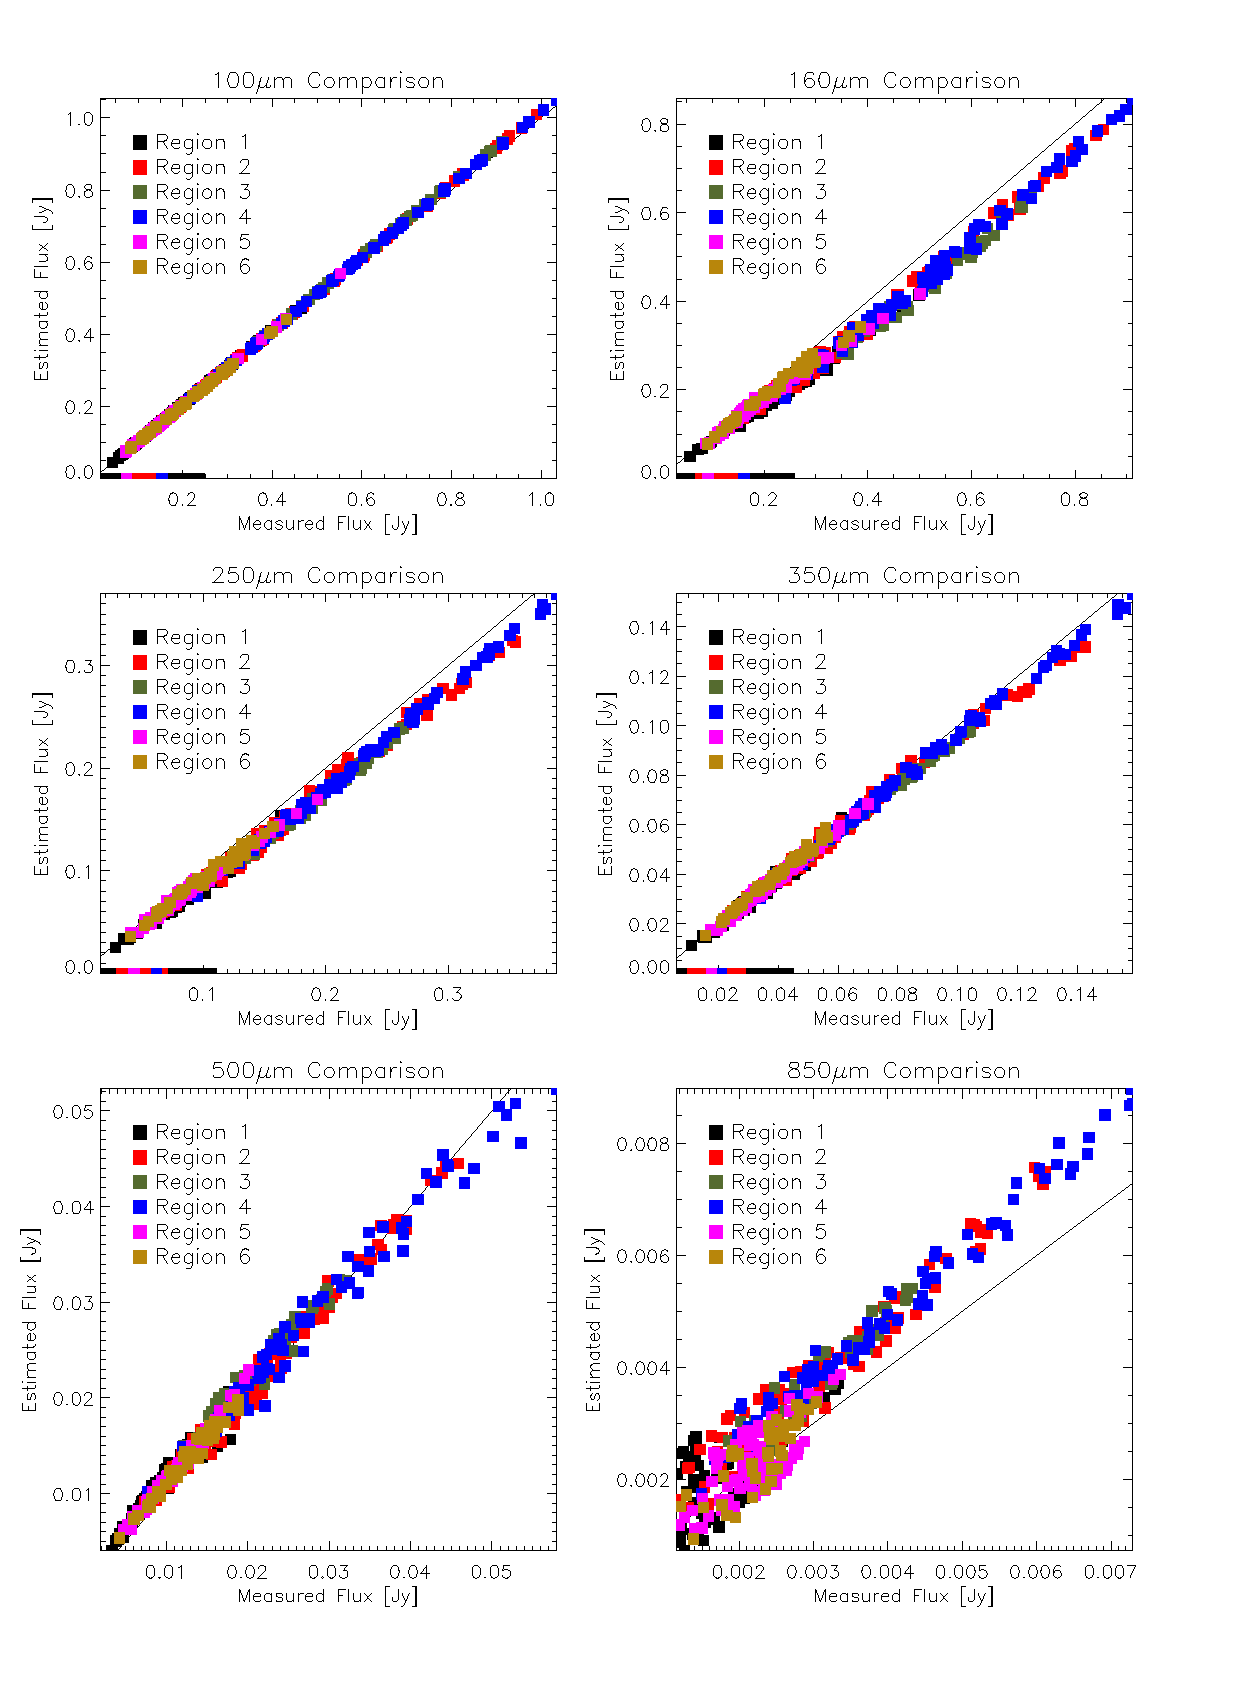
\includegraphics[width=1.\textwidth]{sed_imgs/flux_compare_1_5.eps}
  \caption[Planck Model SED Fit Quality Using 500$\mu$m Data]{Quality of the SED fits using to the Planck model with the 500$\mu$m emission.  The regions shown are the regions in figure \ref{fig:regions}.}
  \label{fig:w1_5}
\end{figure}

\begin{figure}
  \centering
  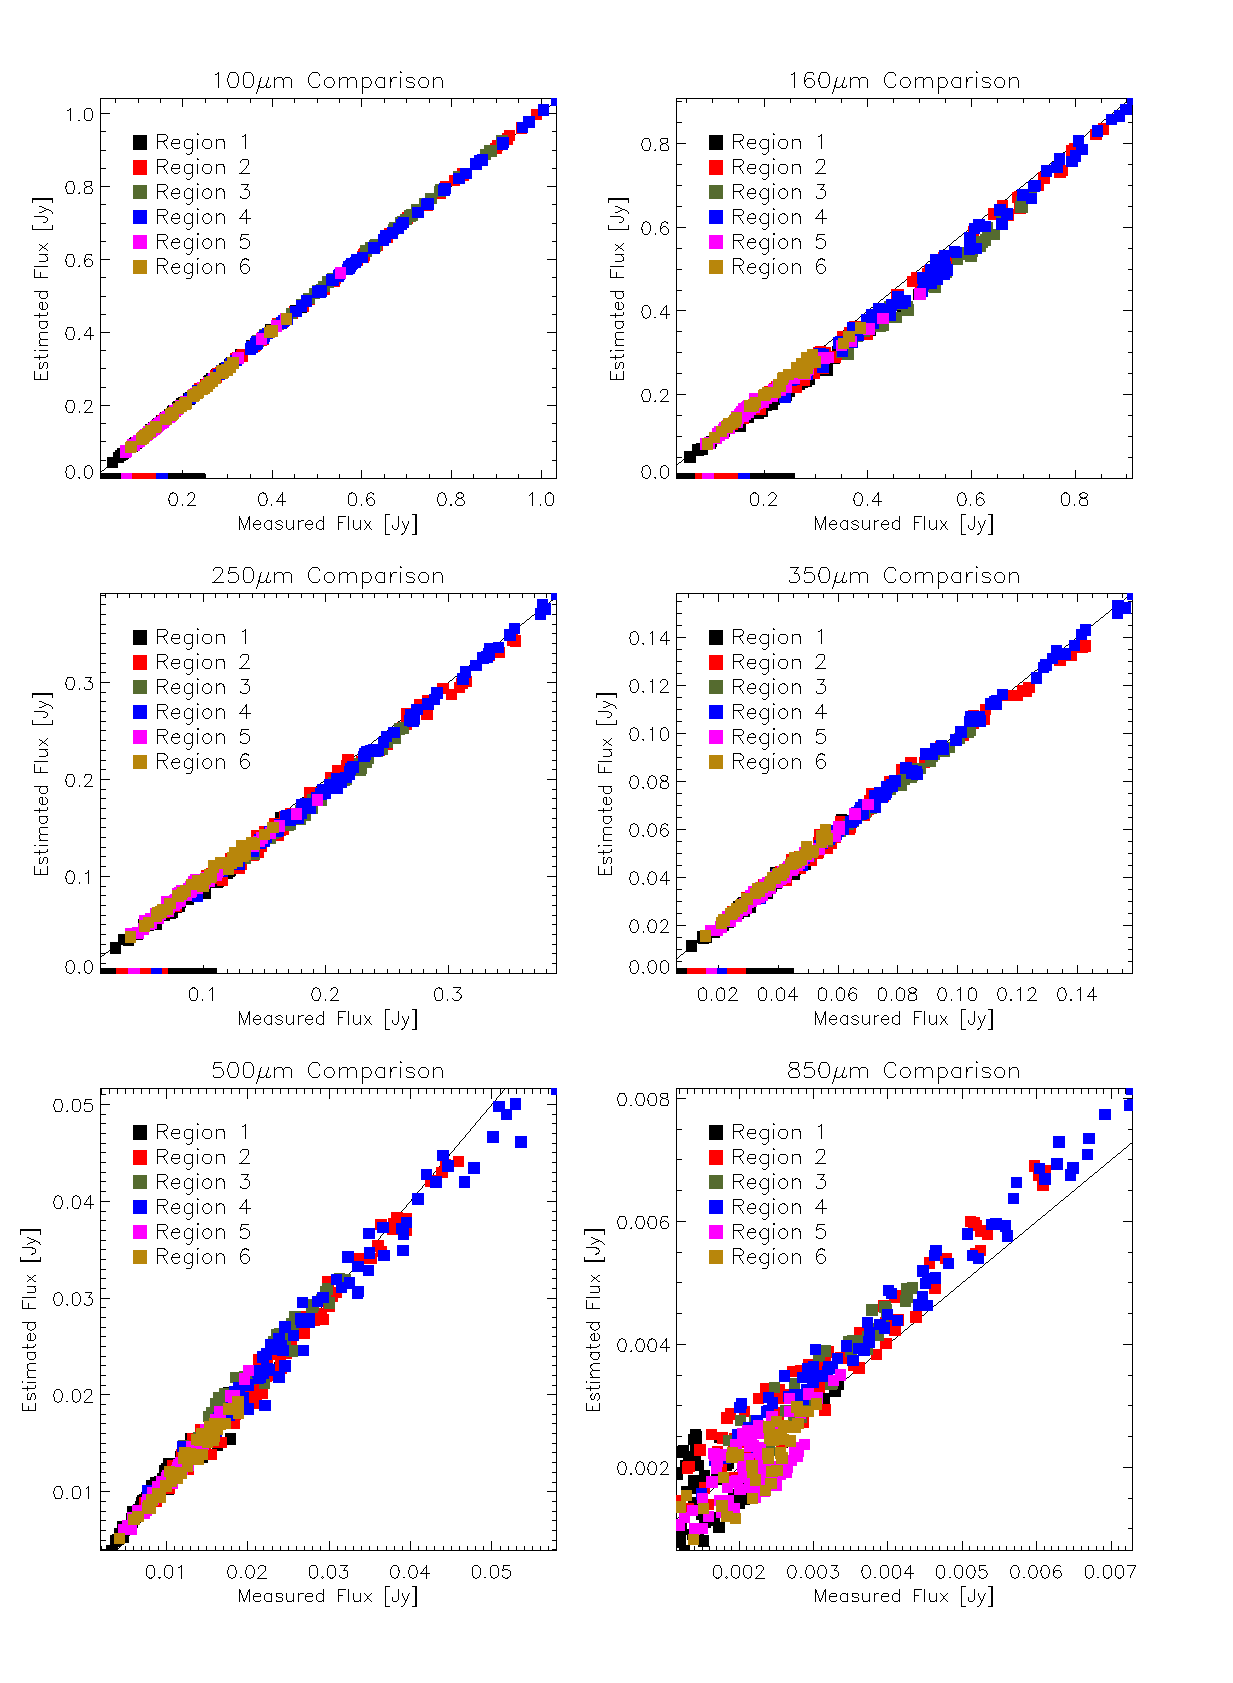
\includegraphics[width=1.\textwidth]{sed_imgs/flux_compare_2_5.eps}
  \caption[Li and Draine Model SED Fit Quality Using 500$\mu$m Data]{Quality of the SED fits using the Planck model with the 500$\mu$m emission.  The regions shown are the regions in figure \ref{fig:regions}.}
  \label{fig:w2_5}
\end{figure}

\begin{figure}
  \centering
  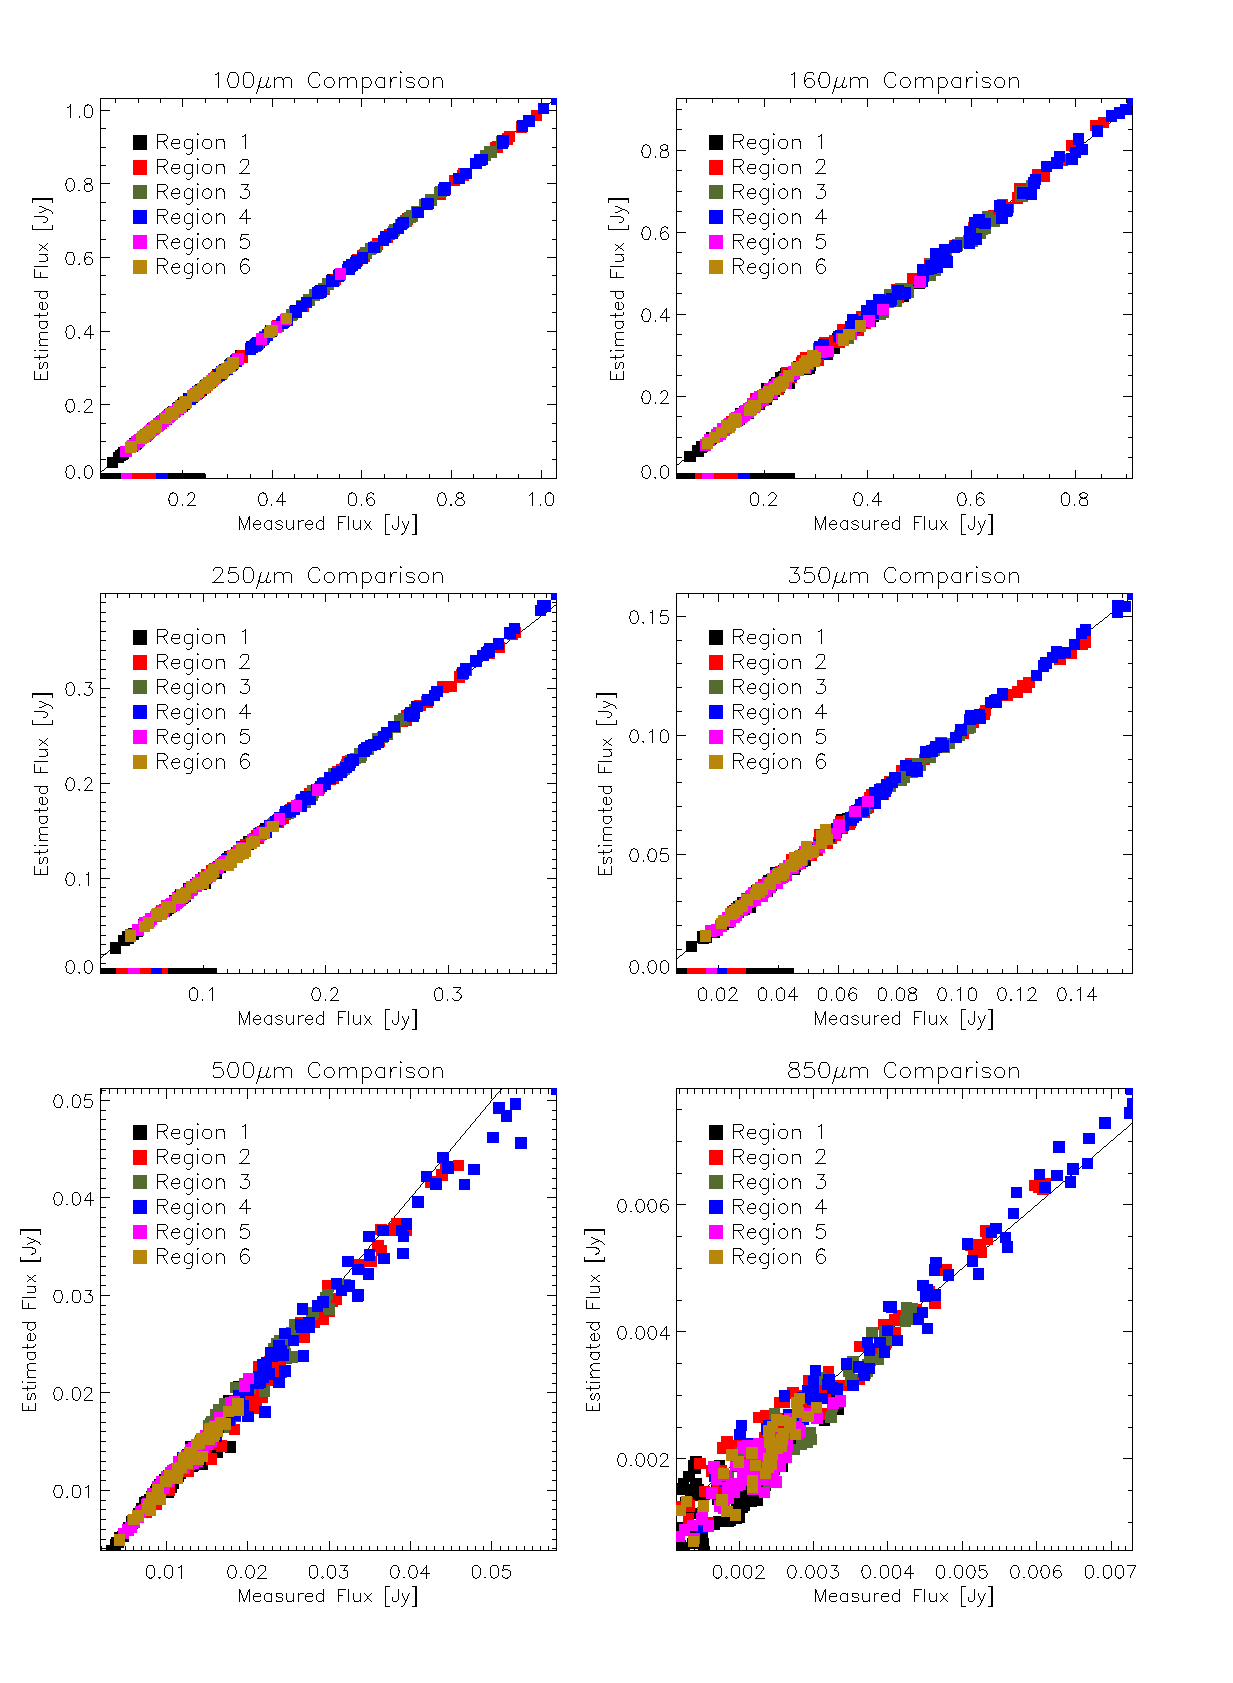
\includegraphics[width=1.\textwidth]{sed_imgs/flux_compare_free_5.eps}
  \caption[Emissivity as a Free Parameter SED Fit Quality using the 500$\mu$m Data]{Quality of the SED fits with the emissivity index as a free paramter with the 500$\mu$m emission.  The regions shown are the regions in figure \ref{fig:regions}.}
  \label{fig:wf_5}
\end{figure}

\begin{deluxetable}{cccc}
  \tablecolumns{4}
  \tablewidth{0pt}
  \tablecaption{Total Distance to 1 to 1 Line\label{tab:lsq}}
  \tablehead{\colhead{Observation} & \colhead{Planck Model} & \colhead{Li and Draine Model} & \colhead{Variable Emissivity Index} }
  \startdata
    100$\mu$m & 0.000   & 0.01245 & 01277   \\
    160$\mu$m & 15.55   & 8.979   & 2.159   \\
    250$\mu$m & 5.808   & 3.072   & 0.4465  \\ 
    350$\mu$m & 0.8045  & 0.3541  & 0.1161  \\
    500$\mu$m & 0.02825 & 0.05218 & 0.09528 \\
    Total     & 23.01   & 12.58   & 3.131   \\
  \enddata
\end{deluxetable}

\subsection{Total Region Flux SED Fits}

The second method used to determine the dust mass, was to fit the SED to the flux of each region in figure \ref{fig:regions}.  Performing the fit in this manner is beneficial because it increases the signal to noise of the region and produces a more precise set of parameters.  Initially, this style of fit was carried in the same fashion as the individual pixel fits  by fixing the emissivity index to 1.8 and 2.0, and allowing the emissivity index to vary.   However, given the greater range of mass values for the region fits, a single valued initial condition for the mass would produce a set of parameters that did not converge to the absolute minimum.  The dependence of the initial mass and the converged parameter with a variable emissivity index are shown in figure \ref{fig:init_mass_bf}.  Similarly, if we fix the emissivity index, the dependence on the initial mass is nonexistent until the Levinberg-Marquardt method is unable to converge to an appropriate fit, figure \ref{fig:init_mass_b1}.

\begin{figure}
  \centering
  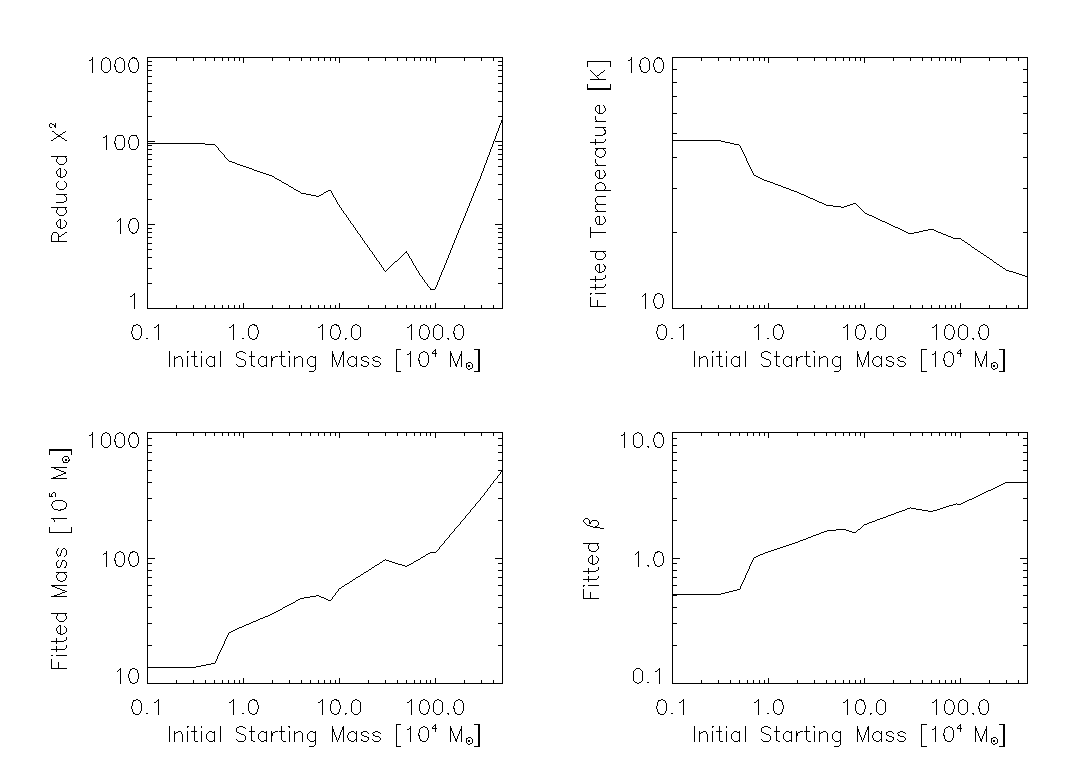
\includegraphics[width=1.\textwidth]{sed_imgs/beta_f_return.eps}
  \caption[Initial Mass Dependence and Convergence of SED Fits for Region Fluxes and Variable Emissivity Index]{Returned SED fitting output with Planck opacity for the $\chi^2$, temperature, mass, and emissivity index with varying initial conditions.  The top left panels shows the $\chi^2$ values for each starting mass.  The top right, bottom left, and bottom right panels show the returned temperatures, mass, and emissivity index.}
  \label{fig:init_mass_bf}
\end{figure}

\begin{figure}
  \centering
  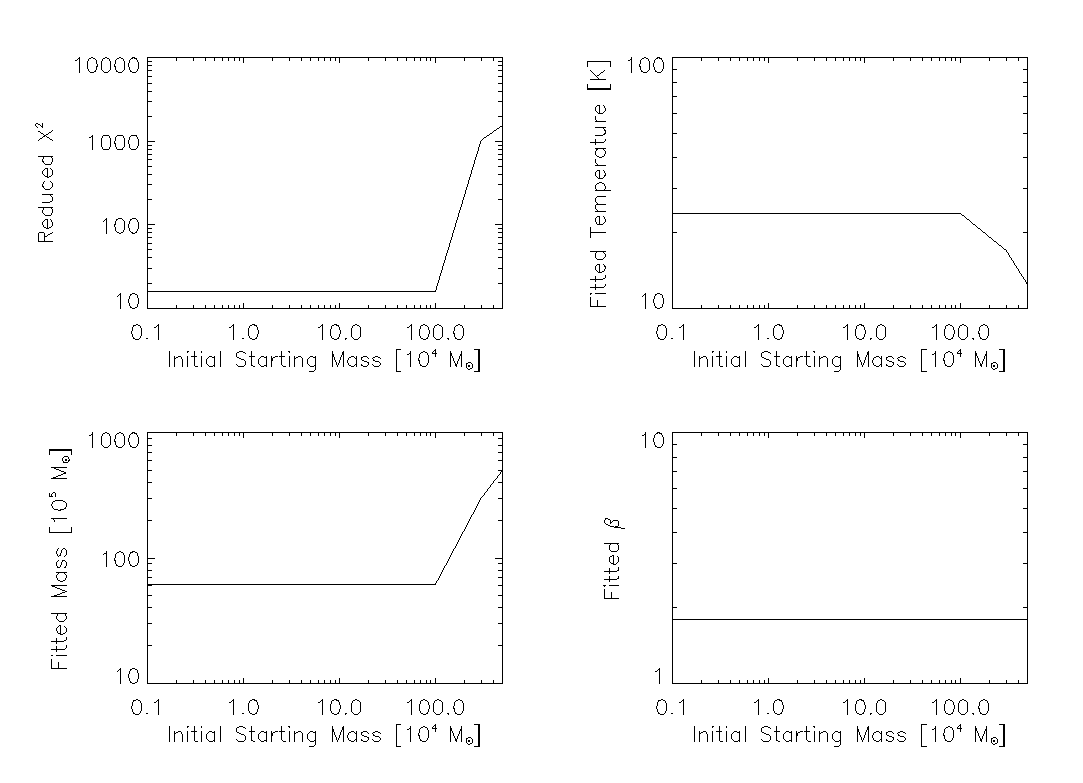
\includegraphics[width=1.\textwidth]{sed_imgs/beta_1_return.eps}
  \caption[Initial Mass Dependence and Convergence of SED Fits for Region Fluxes and Fixed Emissivity Index]{The same as figure \ref{fig:init_mass_bf}, however the emissivity index has been fixed to 1.8.}
  \label{fig:init_mass_b1}
\end{figure}

Since we can't let emissivity index vary freely, an alternative method to determine it's value needs to be implemented.  The emissivity index was determined by fixing it over a range of 1.6 to 2.9 with a spacing of 0.05.  The best emissivity index is determined by which value returns the lowest reduced $\chi^2$.  Plots showing the behavior of the $\chi^2$ values with each emissivity index value are shown in figure \ref{fig:beta_reg_sel} where the best value selected is represented by the red line. The results of each region using the fixed emissivity indices are shown in table \ref{tab:region_vals}, and their resulting SED's are shown in figure \ref{fig:SED_region}.

\begin{figure}
  \centering
  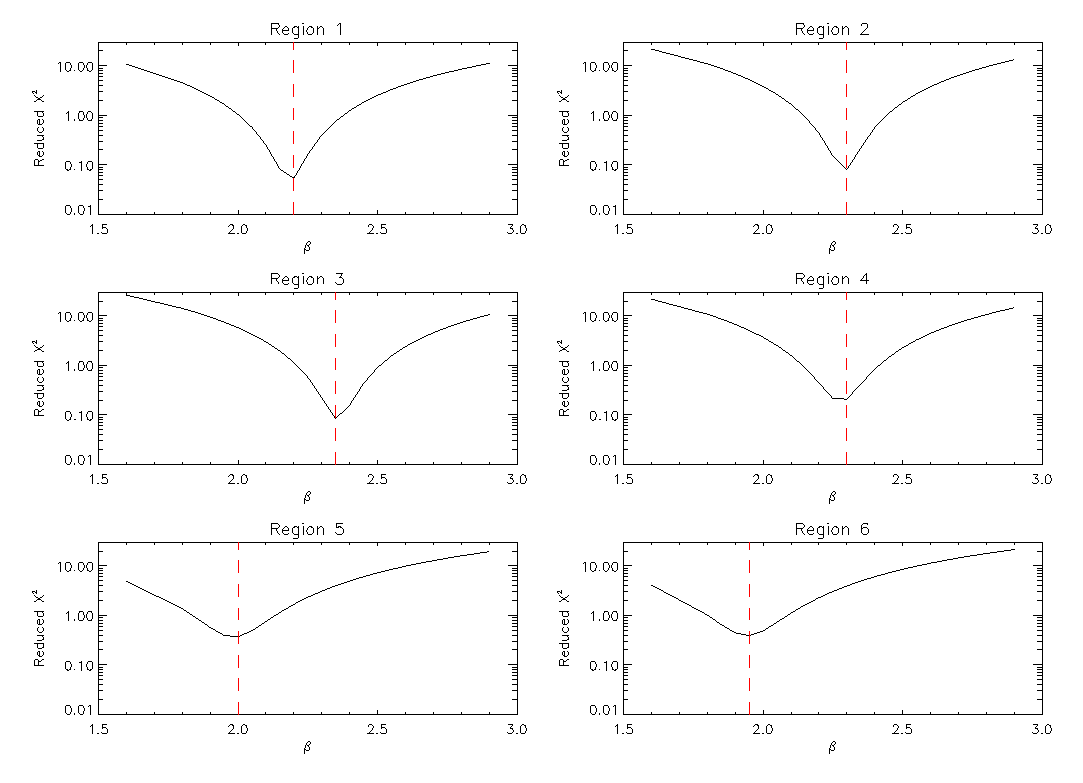
\includegraphics[width=1.\textwidth]{sed_imgs/beta_vals.eps}
  \caption[Region Flux Best Emissivity Index Selection]{Plots for each region from figure \ref{fig:regions} showing the fixed emissivity index value and the resulting reduced $\chi^2$ value.}
  \label{fig:beta_reg_sel}
\end{figure}

\begin{deluxetable}{ccccc}
  \tablecolumns{5}
  \tablewidth{0pt}
  \tablecaption{Best Fit Parameters for Planck Opacity\label{tab:region_vals}}
  \tablehead{\colhead{Region} & \colhead{Average $\beta$} & \colhead{ Total Mass} & \colhead{Surface Density} & \colhead{Average Temperature} \\ & &  $\left[10^5M_\odot\right]$ & $\left[M_\odot pc^{-2}\right]$ &[K]}
  \startdata
    1 & 2.20 $\pm$ 0.03 & 70   $\pm$ 6   & 0.14  $\pm$ 0.01  & 22.8 $\pm$ 0.5 \\
    2 & 2.30 $\pm$ 0.03 & 19   $\pm$ 1   & 0.18  $\pm$ 0.01  & 22.5 $\pm$ 0.3 \\
    3 & 2.35 $\pm$ 0.03 & 9.6  $\pm$ 0.6 & 0.18  $\pm$ 0.01  & 23.3 $\pm$ 0.3 \\
    4 & 2.30 $\pm$ 0.03 & 23   $\pm$ 1   & 0.22  $\pm$ 0.01  & 22.2 $\pm$ 0.2\\
    5 & 2.00 $\pm$ 0.03 & 11.3 $\pm$ 0.8 & 0.092 $\pm$ 0.007 & 22.3 $\pm$ 0.4\\
    6 & 1.95 $\pm$ 0.03 & 4.5  $\pm$ 0.3 & 0.084 $\pm$ 0.006 & 23.9 $\pm$ 0.4 \\
  \enddata
\end{deluxetable}

\begin{figure}
  \centering
  \begin{subfigure}[t]{.48\textwidth}
    \centering
    \includegraphics[width=1.\linewidth]{sed_imgs/region_1beta_22_SED_fit.eps}
    \caption{Region 1 SED}
  \end{subfigure}
  \quad
  \begin{subfigure}[t]{.48\textwidth}
    \centering
    \includegraphics[width=1.\linewidth]{sed_imgs/region_2beta_23_SED_fit.eps}
    \caption{Region 2 SED}
  \end{subfigure}
  
  \begin{subfigure}[t]{.48\textwidth}
    \centering
    \includegraphics[width=1.\linewidth]{sed_imgs/region_3beta_235_SED_fit.eps}
    \caption{Region 3 SED}
  \end{subfigure}
  \quad
  \begin{subfigure}[t]{.48\textwidth}
    \centering
    \includegraphics[width=1.\textwidth]{sed_imgs/region_4beta_23_SED_fit.eps}
    \caption{Region 4 SED}
  \end{subfigure}
  
  \begin{subfigure}[t]{.48\textwidth}
    \centering
    \includegraphics[width=1.\textwidth]{sed_imgs/region_5beta_20_SED_fit.eps}
    \caption{Region 5 SED}
  \end{subfigure}
  \quad
  \begin{subfigure}[t]{.48\textwidth}
    \centering
    \includegraphics[width=1.\textwidth]{sed_imgs/region_6beta_195_SED_fit.eps}
    \caption{Region 6 SED}
  \end{subfigure}
  \caption[Region Flux SED Fits]{SED fits for the flux of each region in figure \ref{fig:regions} using the Planck Opacity.}
  \label{fig:SED_region}
\end{figure}
  
  
  
\section{Discussion}
\subsection{Reliability of Individual Pixel Fits}

The issue on whether or not the individual pixel fits are reliable is raised after seeing a strong dependence with the initial mass of the region SED fits shown in figure \ref{fig:init_mass_bf}.  Since any dependence on the initial mass has been removed in the global region fits, an agreement between the total pixel mass and the region fits would suggest that the initial mass used in the pixel fitting is an appropriate value.  This is further strengthened by the smaller mass range of pixel fits.  The smaller range allows the fitting method to hone into a smaller area of the $\chi^2$ space avoiding any possible local minima to converge on.

\subsection{Comparison with Previous Work}

We can check the validity of our results by comparing them to previous SED fits using the KINGFISH data \citep{galametz2012}.  The best fit parameters from their fitting was T=20.2K$\pm$4K and $\beta$=2.3$\pm$0.2 which agree within error to our results of T=22K$\pm$1K and $\beta$=2.2$\pm$0.2 for a variable emissivity index.  To test agreement with our mass we need to take into account several factors.  The first being a lessened flux from the extended structure removal, and the second is the selection of the opacity value.  Their reported mass for a variable emissivity index reported by \cite{galametz2012} was 782$^{+80}_{-66}\times$10$^5$M$_\odot$ for the sum of pixels in the parameter maps.  We can scale the mass values by finding the ratio $\kappa_{Galametz}$ over $\kappa_{Ours}$ which comes out to be 0.342.  If we then scale by the amount of flux removed in the extended structure removal, we can scale the mass to 175$^{+19}_{-17}\times$10$^5$M$_\odot$ which is above our maximum value of 108$\times$10$^5$M$_\odot$.  This discrepancy can likely be attributed to how the total mass was found in each method.  For our method we use the mass returned from fitting, and in \cite{galametz2012} they use equation \ref{eq:mass} using the 500$\mu$m emssion to determine a dust mass.

%galametz and Draine paper.  Also chris mentioned dwarf galaxy survey shows the 850 excess?

\chapter{Dust-to-Gas Ratio and $\alpha_{CO}$}

\section{Minimizing Scatter Dust-to-Gas Ratio}

In order to determine the amount of molecular hydrogen present, we have chosen to use the dust based method to determine a conversion factor.  In our analysis we have used the conversion factor $\alpha_{CO}$ which will return the amount of molecular hydrogen present in terms of its surface density.  Calculating the amour of molecular hydrogen present with this method involves reducing the scatter of the dust to gas ratio of each pixel.  The dust-to-gas ratio is calculated using

\begin{equation}\label{dgr}
  \delta_{DGR} = \frac{\Sigma_{dust}}{I_{CO}*\alpha_{CO} + \Sigma_{HI}}
\end{equation}

where $\delta_{DGR}$ is the ratio of the surface densities of the dust and gas present in the system, $\Sigma_{dust}$ is the surface density of the dust in M$_\odot$ pc$^{-2}$, $I_{CO}$ is the CO intensity in K km s$^{-1}$, $\alpha_{CO}$ is the conversion factor in units of M$_\odot$ pc$^{-2}$ (K km s$^{-1}$)$^{-1}$, and $\Sigma_{HI}$ is the surface density of the atomic hydrogen.  The scatter of the dust-to-gas ratio is determined by finding the standard deviation of the pixels assuming a Gaussian distribution.  

The ideal configuration was determined using the dust surface densities found in Chapter \ref{sed} for the Planck and Li and Draine models.  The $\alpha_{CO}$ was handled by assigning it a single value over the range of 0.01 to 100 M$_\odot$ pc$^{-2}$ (K km s$^{-1}$)$^{-1}$, and the best approximated $\alpha_{CO}$ was determined by the lowest resulting dust-to-gas scatter in the pixels of each region in Figure \ref{fig:regions}.  A 7$^{th}$ region was added that is the galaxy without the nucleus due to the lack of HI emission in the nucleus of NGC3627.  The surface density of molecular hydrogen is then determined by scaling the CO intensity by the calculated conversion factor, and the dust-to-gas ratio is then found by dividing the dust surface density by the sum of the HI and H$_2$ surface densities.  The results using Planck model with the CO J=1-0 line are shown in Figure \ref{fig:dgr_co10} where the right panel shows the ratio of H$_2$ to HI against the value of the dust-to-gas ratio in each pixel where the solid red line indicates the mean value for the dust-to-gas ratio and the dotted lines show the variance associated with the configuration.  The left panels of Figure \ref{fig:dgr_co10} show the trend of $\alpha_{CO}$ and the scatter in the dust-to-gas ratio.  The numerical values of the dust-to-gas ratio, $\alpha_{CO}$, and H$_2$ surface density using both the Planck and Li and Draine dust masses are shown in Table \ref{tab:dgr_10t}.  The error on the dust to gas ratio  in Table \ref{tab:dgr_10t} is the same as the minimum scatter found.

\begin{figure}\label{fig:dgr_co10}
  \begin{subfigure}[t]{1\textwidth}
    \centering
    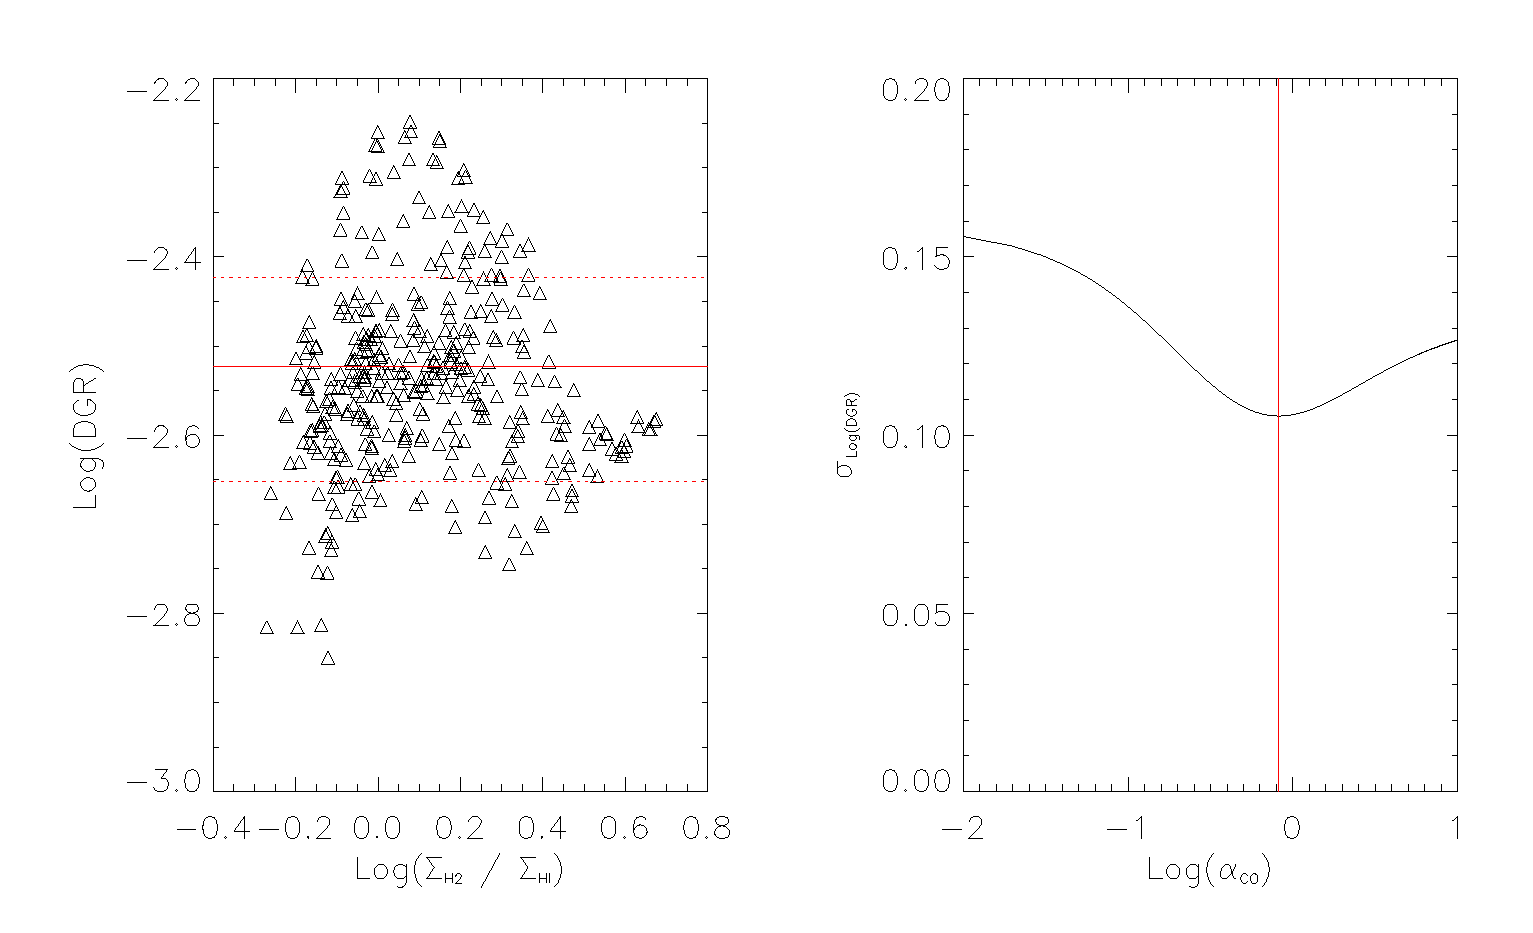
\includegraphics[width=1.\textwidth]{dgr_imgs/region_1_aco_output_10.eps}
    \caption{Region 1}
  \end{subfigure}

  \begin{subfigure}[t]{1\textwidth}
    \centering
    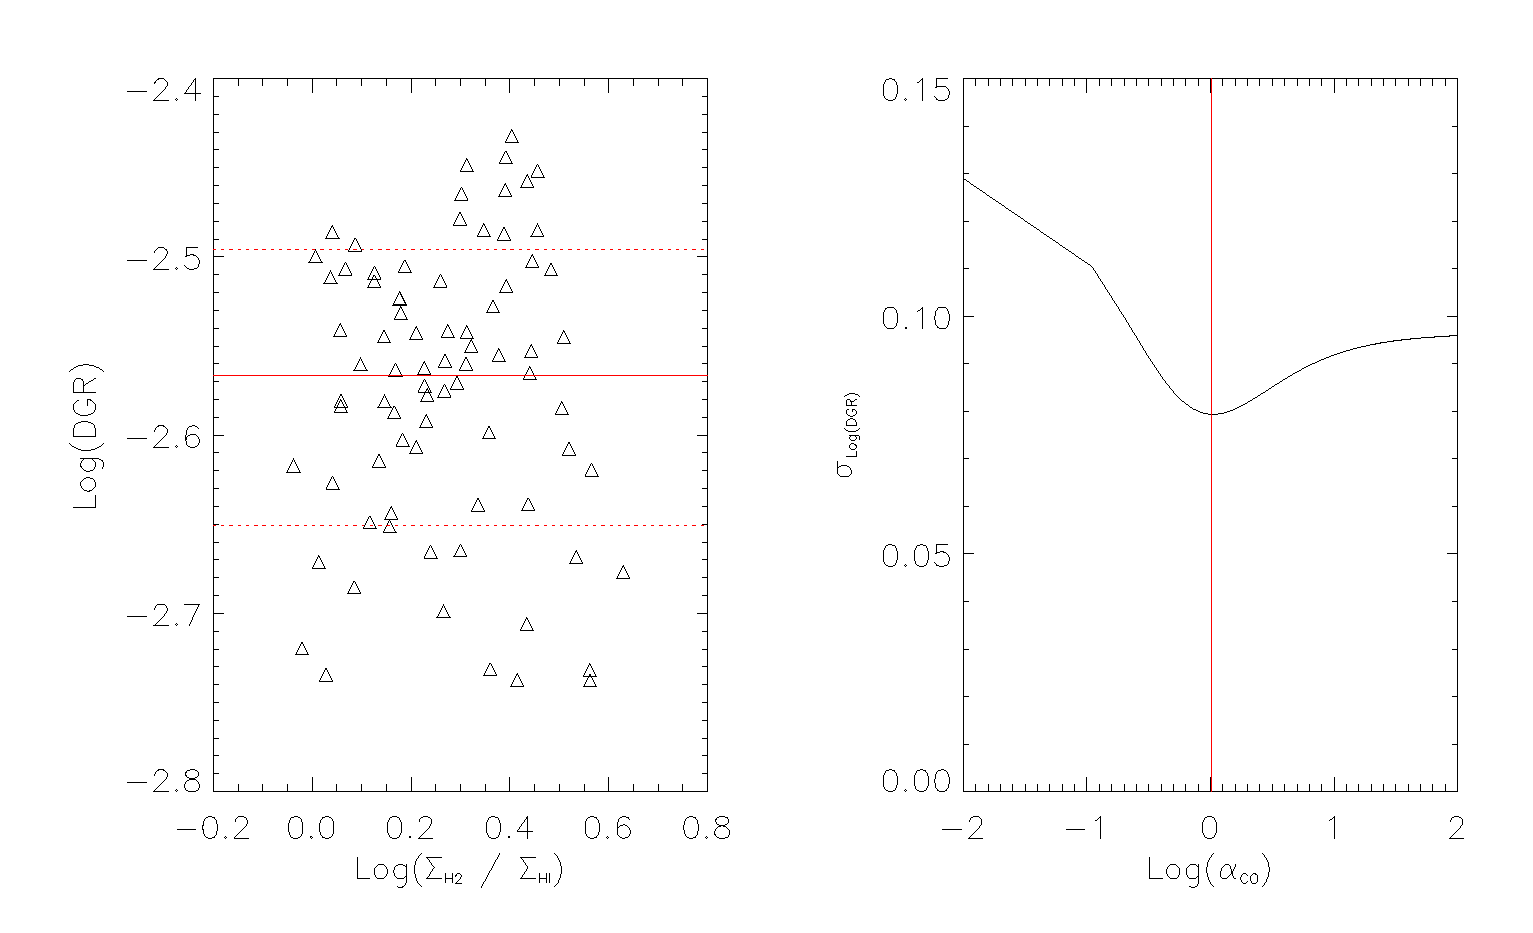
\includegraphics[width=1.\textwidth]{dgr_imgs/region_2_aco_output_10.eps}
    \caption{Region 2}
  \end{subfigure}
   \caption[Dust-to-Gas Ratio Determination Plots for CO J=1-0]{Plots of the dust-to-gas ratio vs the H$_2$ to HI surface densities using the calculated $\alpha_{CO}$ and the scatter in the dust-to-gas ratio against the $\alpha_{CO}$ values used.  Each were calculated using the CO J=1-0 line.}
   \label{fig:dgr_co10}
\end{figure}

\begin{figure}  
  \ContinuedFloat
  \begin{subfigure}[t]{1\textwidth}
    \centering
    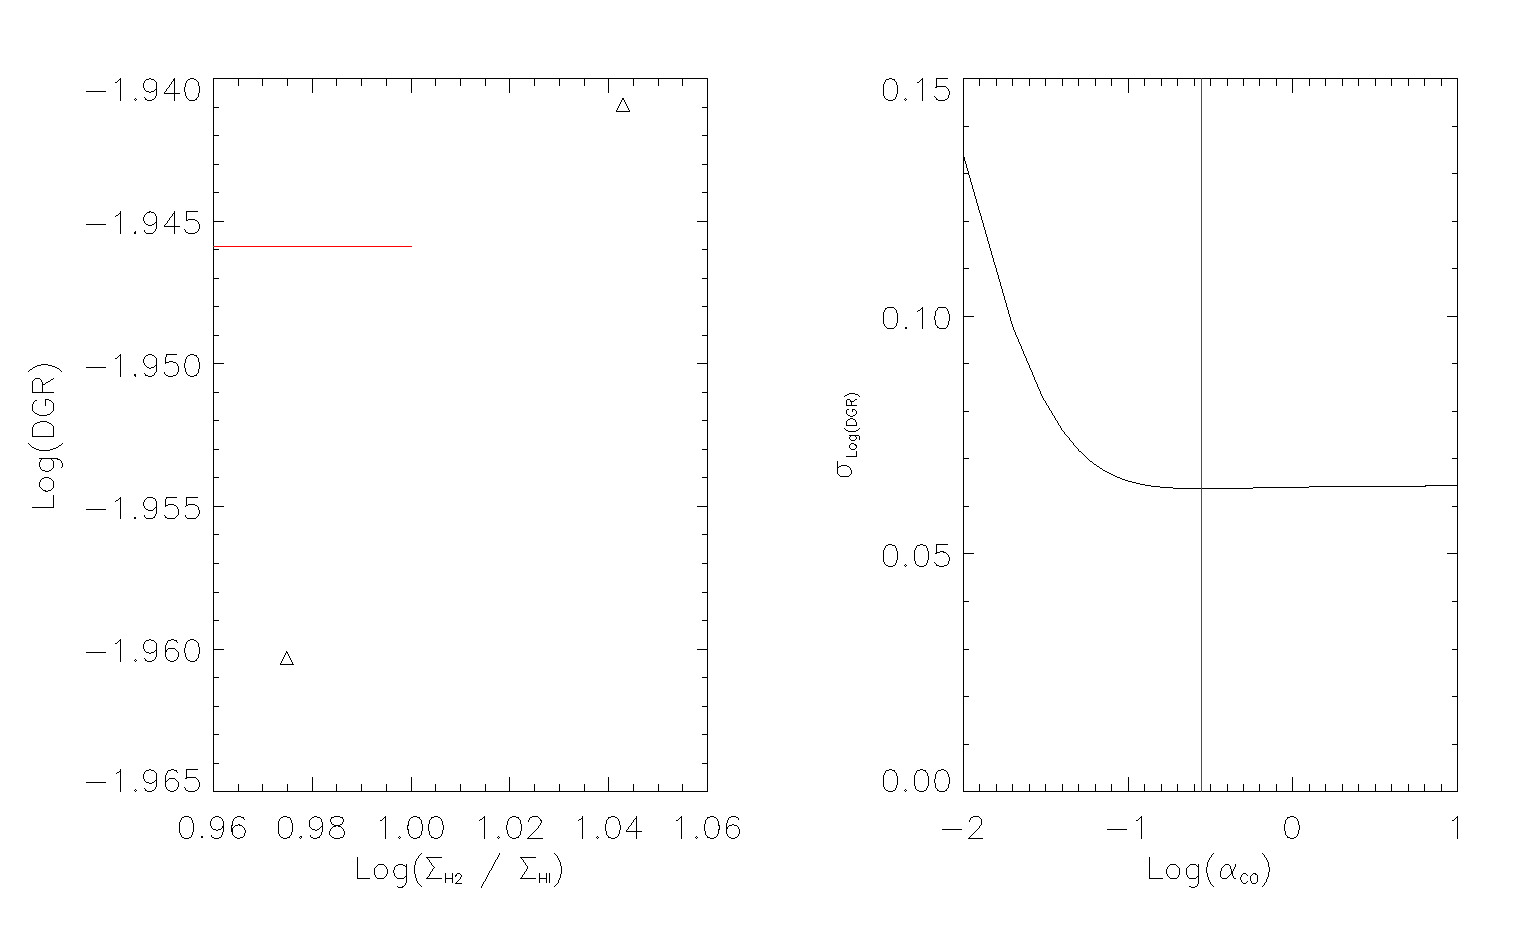
\includegraphics[width=1.\textwidth]{dgr_imgs/region_3_aco_output_10.eps}
    \caption{Region 3}
  \end{subfigure}

  \begin{subfigure}[t]{1\textwidth}
    \centering
    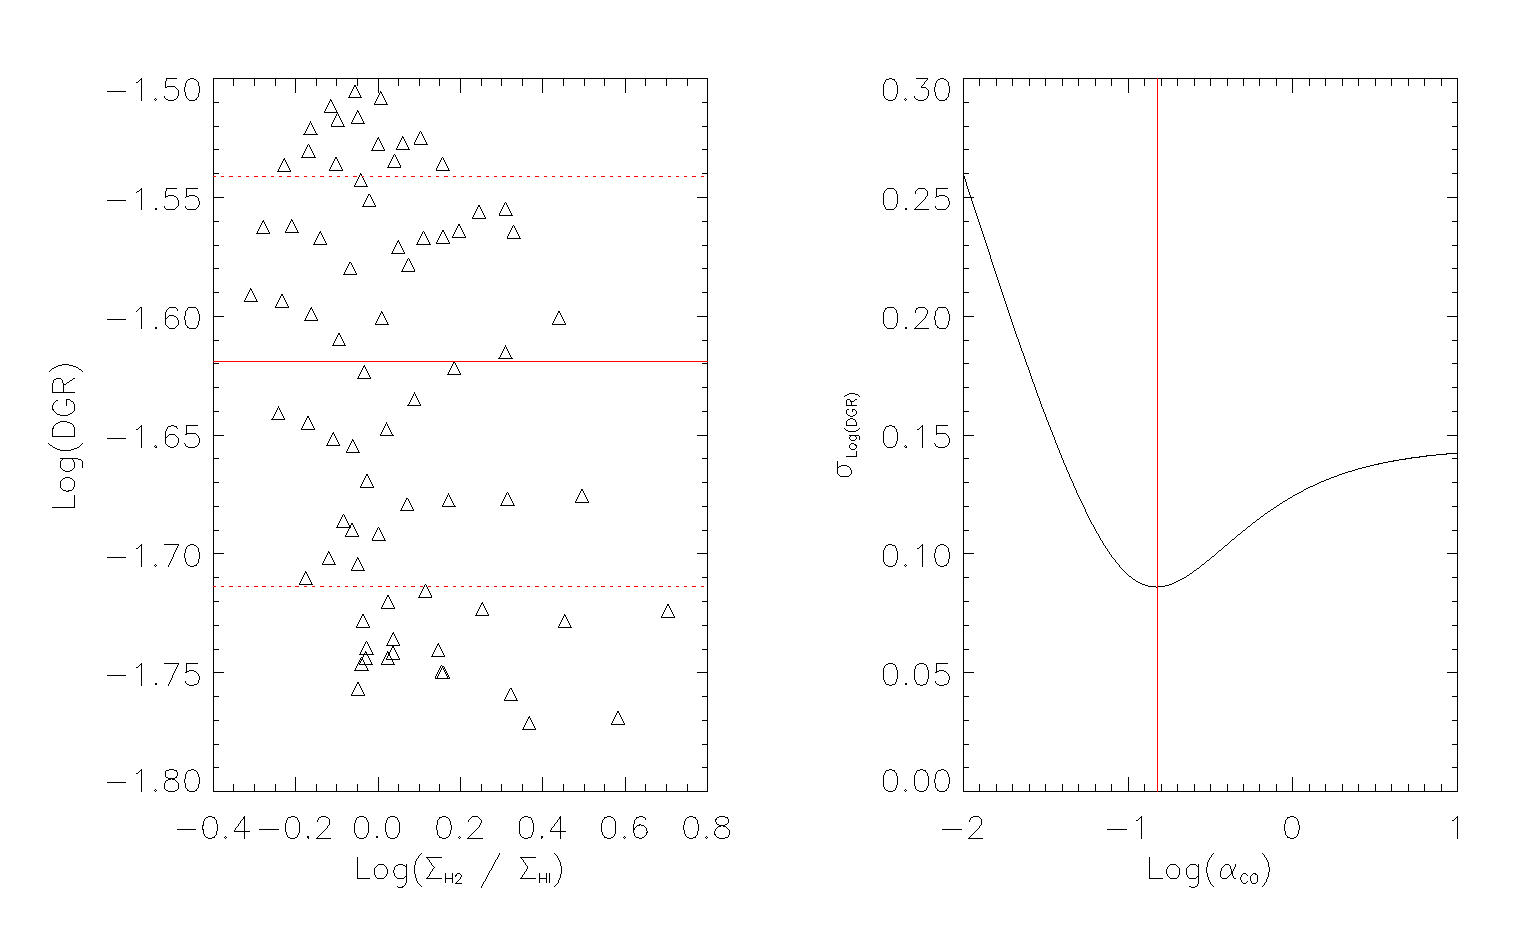
\includegraphics[width=1.\textwidth]{dgr_imgs/region_4_aco_output_10.eps}
    \caption{Region 4}
  \end{subfigure}
   \caption[Dust-to-Gas Ratio Determination Plots for CO J=1-0]{Plots of the dust-to-gas ratio vs the H$_2$ to HI surface densities using the calculated $\alpha_{CO}$ and the scatter in the dust-to-gas ratio against the $\alpha_{CO}$ values used.  Each were calculated using the CO J=1-0 line.}
   \label{fig:dgr_co10}
\end{figure}

\begin{figure}
  \ContinuedFloat
  \begin{subfigure}[t]{1\textwidth}
    \centering
    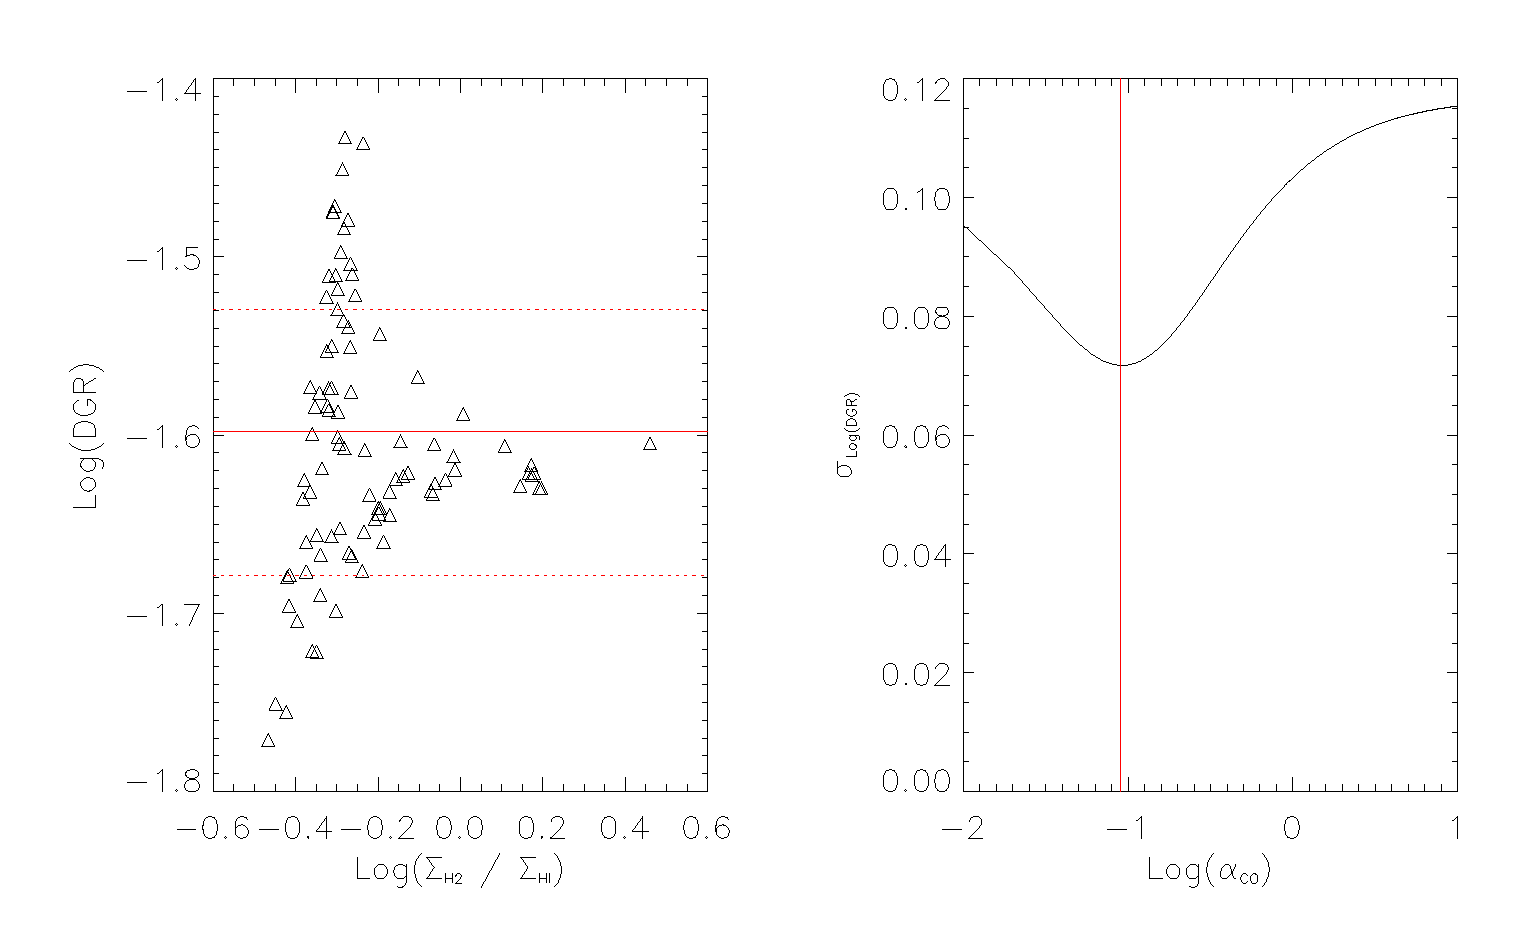
\includegraphics[width=1.\textwidth]{dgr_imgs/region_5_aco_output_10.eps}
    \caption{Region 5}
  \end{subfigure}

  \begin{subfigure}[t]{1\textwidth}
    \centering
    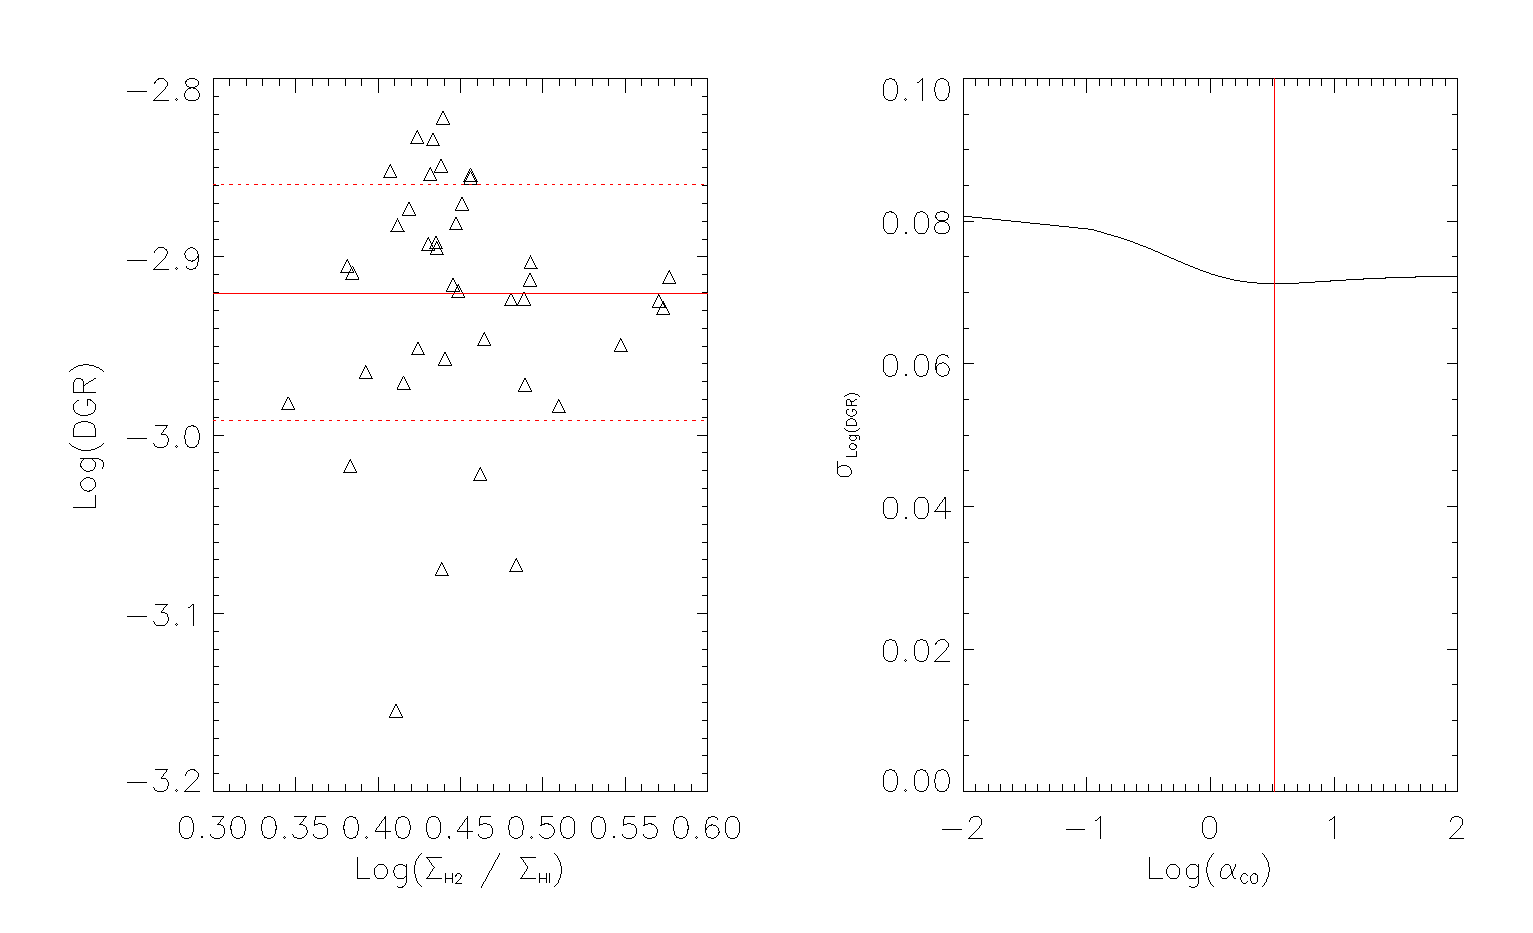
\includegraphics[width=1.\textwidth]{dgr_imgs/region_6_aco_output_10.eps}
    \caption{Region 6}
  \end{subfigure}
   \caption[Dust-to-Gas Ratio Determination Plots for CO J=1-0]{Plots of the dust-to-gas ratio vs the H$_2$ to HI surface densities using the calculated $\alpha_{CO}$ and the scatter in the dust-to-gas ratio against the $\alpha_{CO}$ values used.  Each were calculated using the CO J=1-0 line.}
   \label{fig:dgr_co10}
\end{figure}

\begin{figure}
  \ContinuedFloat
  \begin{subfigure}[t]{1\textwidth}
    \centering
    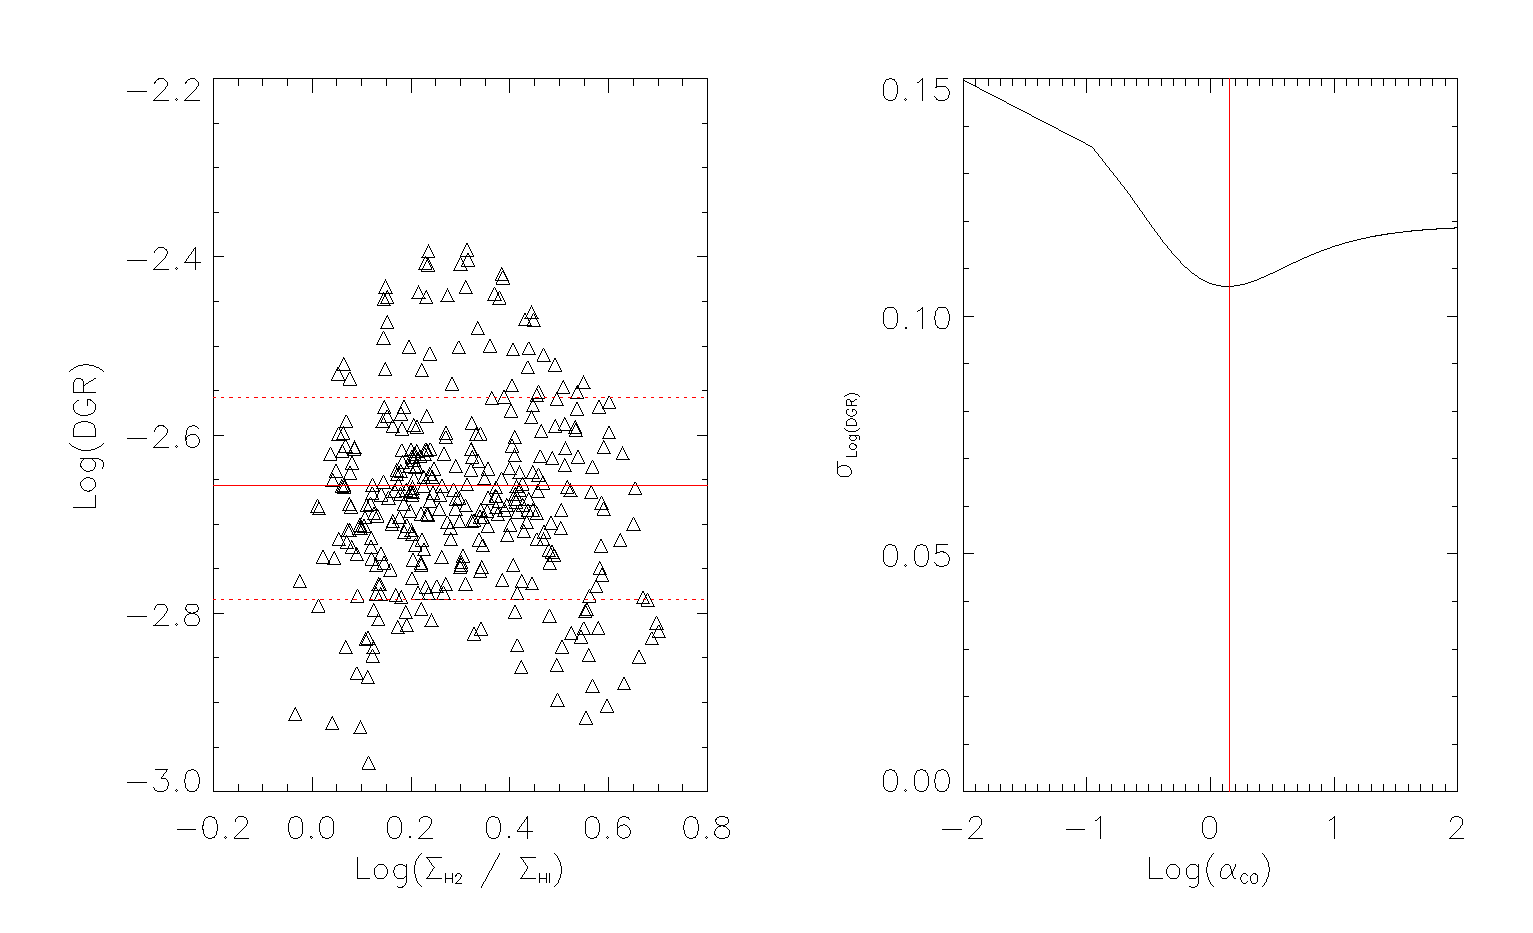
\includegraphics[width=1.\textwidth]{dgr_imgs/region_1-3_aco_output_10.eps}
    \caption{Region 1 Without the Nucleus}
  \end{subfigure}
  \caption[Dust-to-Gas Ratio Determination Plots for CO J=1-0]{Plots of the dust-to-gas ratio vs the H$_2$ to HI surface densities using the calculated $\alpha_{CO}$ and the scatter in the dust-to-gas ratio against the $\alpha_{CO}$ values used.  Each were calculated using the CO J=1-0 line.}
   \label{fig:dgr_co10}
\end{figure}

\begin{deluxetable}{rccc}
  \tabletypesize{\footnotesize}
  \tablecolumns{4}
  \tablewidth{0pt}
  \tablecaption{Dust-to-gas ratio, $\alpha_{CO}$, and H$_2$ Surface Density using CO J=1-0 Tracer\label{tab:dgr_10t}}
  \tablehead{
    \colhead{Opacity Model} &
    \colhead{Dust-to-Gas Ratio} &
    \colhead{$\alpha_{CO}$} &
    \colhead{Average $\Sigma_{H_2}$ per Pixel} \\
    &
    &
    [M$_\odot$ pc$^{-2}$ (K km s$^{-1}$)$^{-1}$] &
    [M$_\odot$ pc$^{-2}$] }
  \startdata
    \sidehead{Region 1}
      Planck &        0.021 $\pm$ 0.005 & 0.150 $\pm$ 0.005 & 3 $\pm$ 2 \\
      Li and Draine & 0.09  $\pm$ 0.02  & 0.160 $\pm$ 0.005 & 3 $\pm$ 2 \\
    \sidehead{Region 2}
      Planck &        0.013 $\pm$ 0.003 & 0.290 $\pm$ 0.005 & 7 $\pm$ 3 \\
      Li and Draine & 0.05  $\pm$ 0.01  & 0.310 $\pm$ 0.005 & 8 $\pm$ 3 \\
    \sidehead{Region 3}
      Planck &        0.038 $\pm$ 0.004 & 0.070 $\pm$ 0.005 & 2.6 $\pm$ 0.6\\
      Li and Draine & 0.17  $\pm$ 0.02  & 0.070 $\pm$ 0.005 & 2.6 $\pm$ 0.6\\
    \sidehead{Region 4}
      Planck &        0.028 $\pm$ 0.005 & 0.110 $\pm$ 0.005 & 3 $\pm$ 1 \\
      Li and Draine & 0.12  $\pm$ 0.02  & 0.110 $\pm$ 0.005 & 3 $\pm$ 1 \\
    \sidehead{Region 5}
      Planck &        0.025 $\pm$ 0.004 & 0.090 $\pm$ 0.005 & 1.2 $\pm$ 0.6\\
      Li and Draine & 0.11  $\pm$ 0.02  & 0.100 $\pm$ 0.005 & 1.4 $\pm$ 0.6\\
    \sidehead{Region 6}
      Planck &        0.009 $\pm$ 0.001 & 0.590 $\pm$ 0.005 & 6 $\pm$ 1 \\
      Li and Draine & 0.040 $\pm$ 0.006 & 0.610 $\pm$ 0.005 & 6 $\pm$ 1 \\
    \sidehead{No Nucleus}
      Planck &        0.019 $\pm$ 0.004 & 0.180 $\pm$ 0.005 & 3 $\pm$ 2 \\
      Li and Draine & 0.08  $\pm$ 0.02  & 0.190 $\pm$ 0.005 & 3 $\pm$ 2 \\
  \enddata
\end{deluxetable}

While CO J=1-0 is the standard molecular tracer of H$_2$ \citep{bolatto2013}, the observations are not always available.  In the situation without CO J=1-0 data an alternative excitation state of CO is used.  This was done by \cite{sandstrom2013} using the CO J=2-1 transition, and by \cite{warren2010} using the CO J=3-2 transition, where the observations were scaled to the expected intensity of the CO J=1-0 using a line ratio.  We have found the line ratio of the 2-1/1-0 to be 0.39 for the galaxy on a whole, and can examine the effects of using this technique to approximate the CO J=1-0 transition in this method.  The results for the dust-to-gas ratio, $\alpha_{CO}$, and H$_2$ surface density are shown in Table \ref{tab:dgr_21}.

\begin{deluxetable}{rccc}
  \tabletypesize{\footnotesize}
  \tablecolumns{4}
  \tablewidth{0pt}
  \tablecaption{Dust-to-gas ratio, $\alpha_{CO}$, and H$_2$ Surface Density using CO J=2-1 Tracer\label{tab:dgr_21}}
  \tablehead{
    \colhead{Opacity Model} &
    \colhead{Dust-to-Gas Ratio} &
    \colhead{$\alpha_{CO}$} &
    \colhead{Average $\Sigma_{H_2}$ per Pixel} \\
    &
    &
    [M$_\odot$ pc$^{-2}$ (K km s$^{-1}$)$^{-1}$] &
    [M$_\odot$ pc$^{-2}$] }
  \startdata
    \sidehead{Region 1}
      Planck &        0.016  $\pm$ 0.002  & 0.630 $\pm$ 0.005 & 5   $\pm$ 3 \\
      Li and Draine & 0.07   $\pm$ 0.01   & 0.670 $\pm$ 0.005 & 5   $\pm$ 3 \\
    \sidehead{Region 2} 
      Planck &        0.0147 $\pm$ 0.007  & 0.650 $\pm$ 0.005 & 6   $\pm$ 3 \\
      Li and Draine & 0.063  $\pm$ 0.003  & 0.680 $\pm$ 0.005 & 7   $\pm$ 3 \\
    \sidehead{Region 3}
      Planck &        0.049  $\pm$ 0.005  & 0.150 $\pm$ 0.005 & 1.9 $\pm$ 0.5 \\
      Li and Draine & 0.21   $\pm$ 0.02   & 0.160 $\pm$ 0.005 & 2.0 $\pm$ 0.6 \\
    \sidehead{Region 4}
      Planck &        0.011  $\pm$ 0.001  & 1.020 $\pm$ 0.005 & 12  $\pm$ 4 \\
      Li and Draine & 0.045  $\pm$ 0.005  & 1.060 $\pm$ 0.005 & 12  $\pm$ 4 \\
    \sidehead{Region 5}
      Planck &        0.013  $\pm$ 0.002  & 0.880 $\pm$ 0.005 & 4  $\pm$ 1\\
      Li and Draine & 0.054  $\pm$ 0.008  & 0.930 $\pm$ 0.005 & 5  $\pm$ 2\\
    \sidehead{Region 6}
      Planck &        0.0109 $\pm$ 0.0008 & 1.140 $\pm$ 0.005 & 4  $\pm$ 1 \\
      Li and Draine & 0.046  $\pm$ 0.004  & 1.180 $\pm$ 0.005 & 5  $\pm$ 1 \\
    \sidehead{No Nucleus}
      Planck &        0.013  $\pm$ 0.002  & 0.830 $\pm$ 0.005 & 6  $\pm$ 4 \\
      Li and Draine & 0.055  $\pm$ 0.008  & 0.880 $\pm$ 0.005 & 6  $\pm$ 4 \\
  \enddata
\end{deluxetable}

\section{Effects of the Dust Model and CO Treatment}

The effects of the dust model are mainly seen in the dust-to-gas ratio for the CO J=1-0 emission.  Since the major difference in the two models was the outputted mass, this would make sense to see the Li and Draine model produce larger dust-to-gas ratios.  The conversion factors show some decrease, but the over all molecular gas surface density all agree within error for each region.  The same trend of larger dust-to-gas ratios are seen when scaling the CO J=2-1 emission the dust-to-gas ratio of the Planck model is larger than the Li and Draine model, however the galaxy as a whole and regions 5 and 6 also show a larger $\alpha_{CO}$ which increases the average surface density of those regions.
  
The effect of the CO treatment shows the same trend trend with the dust models showing that the Li and Draine model yields a higher dust-to-gas ratio, but using the CO J=2-1 emission with a 2-1/1-0 ratio applied significantly increases the conversion factor for each region by a factor of  2 to 10.  Despite the increase in $\alpha_{CO}$ we still see the same masses for all of the regions except for regions 4 and 5.  The conflicting surface densities are due to the behavior of the 2-1/1-0 ratio in these regions.  Region 5 displays a large gradient in 2-1/1-0 ratio as you move south along the spiral arm, and the 75\% percent decrease in region 4 is due to the entire region's 2-1/1-0 ratio is nearly double the mean value of the galaxy.

\section{Validity of Results}

If NGC3627 were to show Milky Way like values, we would expect $\alpha_{CO}\approx$4 \citep{sandstrom2013}.  Except the $\alpha_{CO}$ values given for the the CO J=2-1 emission suggest  NGC3627 is similar to U/LIRG type galaxies whose $\alpha_{CO}$ range has been given as 0.3 - 1.3 M$_\odot$ pc$^{-2}$ (K km s$^{-1}$)$^{-1}$ \citep{downes1998}, and the CO J=1-0 emission falls below the U/LIRG range.  Even our smallest dust-to-gas ratio falls above the typical values found in late type galaxies of 0.005 - 0.01 \citep{smith2012}.  If we compare our results to values recently calculated using the same method by \cite{sandstrom2013}, we find that our conversion factor is much lower than their average of 1.2 M$_\odot$ pc$^{-2}$ (K km s$^{-1}$)$^{-1}$, and our dust-to-gas ratio is much larger than their average of $\approx$0.017.  The low $\alpha_{CO}$ and high dust-to-gas ratios are due mainly to the filtering process applied to our data ($\S$ \ref{ancillary}), in particular the amount of HI removed from the filtering.  If we follow the steps taken in \cite{sandstrom2013} by using the Li and Draine dust model with the CO J=2-1 emission such that none of the gas has been filtered, we get the results shown in Table \ref{tab:no_filt}.

\begin{deluxetable}{cccc}
  \tabletypesize{\footnotesize}
  \tablecolumns{4}
  \tablewidth{0pt}
  \tablecaption{Dust-to-gas ratio, $\alpha_{CO}$, and H$_2$ Surface Density using CO J=2-1 Tracer with no Emission Filtering \label{tab:no_filt}}
  \tablehead{
    \colhead{Region} &
    \colhead{Dust-to-Gas Ratio} &
    \colhead{$\alpha_{CO}$} &
    \colhead{Average $\Sigma_{H_2}$ per Pixel} \\
    &
    &
    [M$_\odot$ pc$^{-2}$ (K km s$^{-1}$)$^{-1}$] &
    [M$_\odot$ pc$^{-2}$] }
  \startdata
      1 & 0.010   $\pm$ 0.001   & 3.890 $\pm$ 0.005 & 31 $\pm$ 18 \\
      2 & 0.0107  $\pm$ 0.0009  & 3.470 $\pm$ 0.005 & 36 $\pm$ 15 \\
      3 & 0.0174  $\pm$ 0.0009  & 1.380 $\pm$ 0.005 & 19 $\pm$ 5  \\
      4 & 0.013   $\pm$ 0.001   & 3.000 $\pm$ 0.005 & 36 $\pm$ 12 \\
      5 & 0.0085  $\pm$ 0.0009  & 5.080 $\pm$ 0.005 & 28 $\pm$ 9  \\
      6 & 0.0065  $\pm$ 0.0007  & 7.930 $\pm$ 0.005 & 35 $\pm$ 10 \\
      No Nucleus & 0.0076  $\pm$ 0.0009  & 5.780 $\pm$ 0.005 & 44 $\pm$ 25 \\
  \enddata
\end{deluxetable}
 

\chapter{Summary}

We have shown two new continuum maps of NGC3627 in 450$\mu$m and 850$\mu$m from SCUBA-2, and analyzed them with the goal of determining a dust-to-gas mass ratio, a suitable conversion factor, and the amount of molecular hydrogen present in the galaxy as a whole and 5 individual regions picked based upon the morphological features of the galaxy.  In order to produce our results we utilized data from the KINGFISH survey \citep{kennicutt2011} and NGLS \citep{wilson2012} to calculate a dust mass using SED fitting on a pixel by pixel scale and a total of the flux.  The dust-to-gas ratio, $\alpha_{CO}$, and molecular gas surface density was determined using a minimization of the dust-to-gas scatter in the galaxy using dat, Nobeyama 45-m CO J=1-0 survey \citep{kuno2007}, HERACLES \citep{reuter1996}, and THINGS \citep{walter2008}.  The important results from our analysis are as follows:

\begin{enumerate}

\item{We have created high quality images of NGC3627 using the Starlink program MAKEMAP by incorporating masks in the AST and FLT portions of MAKEMAP and adding a high-pass filter of 175$\arcsec$ to in the FLT portion of MAKEMAP in order to reduce the noise in the final image products.}

\item{Using results from the KINGFISH survey \citep{kennicutt2011}, we were able to show an excess emission was present in the 450$\mu$m observations that was most likely due to calibration issue rather than a physical process in the ISM of NGC3627.}

\item{The results of the SED analysis were tested using two competing dust models calculated by the Planck observation group \citep{planckxxv2011}, Li and Draine \citep{li2001}, and the third model was tested using the opacity values from the Planck model with an emissivity index that was allowed to vary over 5 regions of NGC3627 and the galaxy as a whole.  The results are shown in Tables \ref{tab:beta_1}, \ref{tab:beta_2}, \ref{tab:beta_f}, and \ref{tab:region_vals}.  The calculated temperatures for the entire galaxy are 23$\pm$2 K, 24$\pm$2 K, 22$\pm$1 K, and 22$\pm$2 K for the Planck model, Li and Draine model, free emissivity index, and regional flux, respectively.  The calculated masses using the Planck opacity are 52$\pm$23 M$_\odot$, 73$\pm$31 M$_\odot$, and 75$\pm$28 M$_\odot$ for the Planck model, free emissivity index and regional flux, respectively.  The mass returned for the Li and Draine model is 230$\pm$103 M$_\odot$.  When the emissivity index was allowed to vary the returned values were 2.2$\pm$0.2 and 2.3$\pm$0.3 for the pixel by pixel fits and regional flux, respectively.  The results from the fitting agreed with previous fittings by \cite{galametz2012}.}

\item{There was no observed excess of emission at 850$\mu$m in our fits, which contradict the results of \cite{galametz2014} using 870$\mu$m emission from LABOCA.  The difference in results can be attributed to their handling of the molecular contribution and whether the reduction process of the 870$\mu$m emission preserves extended features.}

\item{Varying dust models used in determining the dust-to-gas ratio showed that the Li and Draine model yielded higher dust-to-gas ratios than the Planck model.  This is due to the Li and Draine model having a higher dust surface density.}

\item{Using either the CO J=1-0 or scaling the CO J=2-1 using a 2-1/1-0 ratio will not effect the dust-to-gas ratio, but will change the conversion factor.  Using the scaled CO J=2-1 emission will provide higher conversation factors because the CO J=1-0 emission will trace more diffuse gas \citep{wilson1990} where atomic hydrogen will be more dominant than its molecular counterpart.}

\item{The gas data with the extended emission removed yielded $\alpha_{CO}$ values typical of U/LIRGs.  This was due to the significant portion of the HI emission that is made up of extended emission.  When using unfiltered gas data, we recovered conversion factors within the vicinity of \cite{sandstrom2013}.  The dust-to-gas ratios however were much smaller than the reported values of \cite{sandstrom2013}.  The lower gas-to-dust ratios is attributed to a larger dust mass that contains not only the cold component we used, but their analysis also include the warm component and PAH contribution.}

\end{enumerate}

Future on the NGC3627 and SCUBA-2 data would include:

\begin{enumerate}

\item{Investing the excess of emission at the 450$\mu$m to determine its source.  If the unphysical excess 450$\mu$m could be found, the resolution of this analysis could be reduced and higher quality SED fitting could take place.}

\item{Implementing a MCMC method to determine an $\alpha_{CO}$ values for each pixel would help to decrease the overall scatter of the dust-to-gas ratio and provide dust-to-gas ratio, $\alpha_{CO}$, and H$_2$ surface density maps to go with the SED fitting maps.  These maps could be used to determine correlations in $\alpha_{CO}$ with parameters returned from the SED fitting.}

\item{Implementing this analysis on other targets in the NGLS catalogue would allow for a large scale  statistical survey over the properties of the dust in the local Universe.}

\end{enumerate}

\appendix
\bibliography{references2}
\bibliographystyle{Styles/apj}
\addtocounter{page}{-1}
\label{finalpage}

\clearpage
%\vspace*{0.3\textheight}
%\begin{center}
%{\Large\bf
%This page intentionally left blank.
%
%}
%end{center}
\end{document}
%\end


